% Options for packages loaded elsewhere
\PassOptionsToPackage{unicode}{hyperref}
\PassOptionsToPackage{hyphens}{url}
\PassOptionsToPackage{dvipsnames,svgnames,x11names}{xcolor}
%
\documentclass[
  letterpaper,
  DIV=11,
  numbers=noendperiod]{scrartcl}

\usepackage{amsmath,amssymb}
\usepackage{setspace}
\usepackage{iftex}
\ifPDFTeX
  \usepackage[T1]{fontenc}
  \usepackage[utf8]{inputenc}
  \usepackage{textcomp} % provide euro and other symbols
\else % if luatex or xetex
  \usepackage{unicode-math}
  \defaultfontfeatures{Scale=MatchLowercase}
  \defaultfontfeatures[\rmfamily]{Ligatures=TeX,Scale=1}
\fi
\usepackage{lmodern}
\ifPDFTeX\else  
    % xetex/luatex font selection
\fi
% Use upquote if available, for straight quotes in verbatim environments
\IfFileExists{upquote.sty}{\usepackage{upquote}}{}
\IfFileExists{microtype.sty}{% use microtype if available
  \usepackage[]{microtype}
  \UseMicrotypeSet[protrusion]{basicmath} % disable protrusion for tt fonts
}{}
\usepackage{xcolor}
\setlength{\emergencystretch}{3em} % prevent overfull lines
\setcounter{secnumdepth}{5}
% Make \paragraph and \subparagraph free-standing
\ifx\paragraph\undefined\else
  \let\oldparagraph\paragraph
  \renewcommand{\paragraph}[1]{\oldparagraph{#1}\mbox{}}
\fi
\ifx\subparagraph\undefined\else
  \let\oldsubparagraph\subparagraph
  \renewcommand{\subparagraph}[1]{\oldsubparagraph{#1}\mbox{}}
\fi


\providecommand{\tightlist}{%
  \setlength{\itemsep}{0pt}\setlength{\parskip}{0pt}}\usepackage{longtable,booktabs,array}
\usepackage{calc} % for calculating minipage widths
% Correct order of tables after \paragraph or \subparagraph
\usepackage{etoolbox}
\makeatletter
\patchcmd\longtable{\par}{\if@noskipsec\mbox{}\fi\par}{}{}
\makeatother
% Allow footnotes in longtable head/foot
\IfFileExists{footnotehyper.sty}{\usepackage{footnotehyper}}{\usepackage{footnote}}
\makesavenoteenv{longtable}
\usepackage{graphicx}
\makeatletter
\def\maxwidth{\ifdim\Gin@nat@width>\linewidth\linewidth\else\Gin@nat@width\fi}
\def\maxheight{\ifdim\Gin@nat@height>\textheight\textheight\else\Gin@nat@height\fi}
\makeatother
% Scale images if necessary, so that they will not overflow the page
% margins by default, and it is still possible to overwrite the defaults
% using explicit options in \includegraphics[width, height, ...]{}
\setkeys{Gin}{width=\maxwidth,height=\maxheight,keepaspectratio}
% Set default figure placement to htbp
\makeatletter
\def\fps@figure{htbp}
\makeatother

\usepackage{fontspec}
\usepackage{multirow}
\usepackage{multicol}
\usepackage{colortbl}
\usepackage{ulem}
\usepackage{hhline}
\newlength\Oldarrayrulewidth
\newlength\Oldtabcolsep
\usepackage{longtable}
\usepackage{array}
\usepackage{hyperref}
\usepackage{float}
\usepackage{wrapfig}
% \usepackage{hyperref}
% \hypersetup{
%     colorlinks,
%     linkcolor={blue!100!black},
%     citecolor={blue!100!black},
%     urlcolor={blue!100!black}
% }
% \usepackage{apacite}
% \usepackage[round]{natbib} 
% \usepackage{graphicx}
% \usepackage{float}
% \usepackage{caption}
% \usepackage[toc,page]{appendix}
% \usepackage{booktabs,caption}
% \usepackage[flushleft]{threeparttable}
% \usepackage{tabularx}
\usepackage{sfmath}
\usepackage{fontspec}
\usepackage[utf8]{inputenc}
\usepackage{siunitx}
\usepackage{amsfonts}
\usepackage{amsmath}
% \usepackage{xcolor}
% \usepackage{scrextend}
% \deffootnote[2em]{2em}{1em}{\textsuperscript{\thefootnotemark}\,}
% \newcolumntype{Y}{>{\centering\arraybackslash}X}
% \usepackage[a4paper]{geometry}
% \usepackage{caption}
% \usepackage[bottom,flushmargin,hang,multiple]{footmisc}
% \usepackage{pdflscape}
% \usepackage[paper=portrait,pagesize]{typearea}
% \usepackage{rotating}
% \usepackage{fullpage}
% \usepackage{tabu}
\usepackage{lscape}
\newcommand{\blandscape}{\begin{landscape}}
\newcommand{\elandscape}{\end{landscape}}
\usepackage{rotating}
\newcommand{\bsideways}{\begin{sidewaystable}[htbp]}
\newcommand{\esideways}{\end{sidewaystable}}
\KOMAoption{captions}{tableheading}
\makeatletter
\@ifpackageloaded{caption}{}{\usepackage{caption}}
\AtBeginDocument{%
\ifdefined\contentsname
  \renewcommand*\contentsname{Table of contents}
\else
  \newcommand\contentsname{Table of contents}
\fi
\ifdefined\listfigurename
  \renewcommand*\listfigurename{List of Figures}
\else
  \newcommand\listfigurename{List of Figures}
\fi
\ifdefined\listtablename
  \renewcommand*\listtablename{List of Tables}
\else
  \newcommand\listtablename{List of Tables}
\fi
\ifdefined\figurename
  \renewcommand*\figurename{Figure}
\else
  \newcommand\figurename{Figure}
\fi
\ifdefined\tablename
  \renewcommand*\tablename{Table}
\else
  \newcommand\tablename{Table}
\fi
}
\@ifpackageloaded{float}{}{\usepackage{float}}
\floatstyle{ruled}
\@ifundefined{c@chapter}{\newfloat{codelisting}{h}{lop}}{\newfloat{codelisting}{h}{lop}[chapter]}
\floatname{codelisting}{Listing}
\newcommand*\listoflistings{\listof{codelisting}{List of Listings}}
\makeatother
\makeatletter
\makeatother
\makeatletter
\@ifpackageloaded{caption}{}{\usepackage{caption}}
\@ifpackageloaded{subcaption}{}{\usepackage{subcaption}}
\makeatother
\ifLuaTeX
  \usepackage{selnolig}  % disable illegal ligatures
\fi
\usepackage[round]{natbib}
\bibliographystyle{apalike}
\usepackage{bookmark}

\IfFileExists{xurl.sty}{\usepackage{xurl}}{} % add URL line breaks if available
\urlstyle{same} % disable monospaced font for URLs
\hypersetup{
  colorlinks=true,
  linkcolor={blue!100!black},
  filecolor={Maroon},
  citecolor={blue!100!black},
  urlcolor={blue!100!black},
  pdfcreator={LaTeX via pandoc}}

\author{}
\date{}

\begin{document}

\title{Inflation Dynamics and Relative Price Dispersion in South Africa: Implications for Optimal Inflation Targeting}



\date{\today}
\maketitle

\begin{abstract}
This paper investigates the dynamic relationship between inflation and relative price dispersion (RPD) in South Africa, focusing on the period from 2009 to 2025, a timeframe marked by significant structural changes in inflation targeting. Drawing on both theoretical models—the menu cost and signal extraction frameworks—the study tests their predictions on how inflation influences RPD using a semi-parametric approach. It extends the analysis by employing quantile-on-quantile regression to capture state-dependent effects across the distribution of relative price variability. The South African case is particularly insightful due to its evolving inflation targets, transitioning from a 3-6 percent band (2000) to a 4.5 percent midpoint target (2017), and moving towards a 3 percent target projected for 2025. These policy shifts offer a unique opportunity to explore the nonlinear, U-shaped nature of the inflation-RPD relationship, challenging the traditional view that zero inflation is optimal. Empirically, this study contributes to the scant emerging market literature, complementing prior work but incorporating inflation target changes. The findings have important implications for monetary policy design in emerging economies aiming to lower inflation targets while minimizing distortive effects on price signals and resource allocation.
\end{abstract}

\noindent\textbf{Keywords}: Relative Price Dispersion, Inflation, Monetary Policy\\
\textbf{JEL Codes}: E31, E52, E58
\newpage

\setstretch{1.5}
\section{Introduction}\label{introduction}

Inflation is known to have adverse welfare effects through its
distortion of relative prices which causes the mis-allocation of
resources, production inefficiencies leading to lower real economic
activity. This is well supported by both theoretical and empirical
studies. This paper contributes to the empirical literature, by
examining the relationship between inflation and relative price
dispersion (RPD) in South Africa given the little evidence available and
to determine how the relationship has evolved given inflation target
changes and its implications for monetary policy.

The South African context can provide further insights into the
relationship between inflation and RPD given the changes in the
inflation targets from a 3 to 6 per cent band in 2000 to a 4.5 per cent
midpoint target since 2017 and a shift to 3 per cent inflation target in
2025 as structural changes in inflation can affect the linkages with
relative price dispersion \citep{caglayan2003}. Furthermore, that the
functional form of relationship is U-shaped and dynamic
\citep{fielding2000, choi2010} implying a non-zero optimal inflation
rate that minimizes the distortive effect on relative prices since a
linear relationship would imply that the optimal inflation rate is zero.
Given the above mentioned inflation target reforms, South Africa
provides an opportunity to examine the dynamic effects of inflation on
relative price variability and the optimal inflation target with policy
implications for emerging market economies that intend to transition to
lower inflation targets.

The theoretical literature distinguishes between menu-cost and signal
extraction models in explaining the positive relation between inflation
and RPD. In menu cost models
\citep{sheshinki1979, sheshinski1983, rotemberg1983, benabou1992} firms
face fixed cost of adjusting nominal prices (e.g.~printing new menus)
and since they follow a one-sided dynamic pricing rule (S, s) when
setting prices, inflation reduces the optimal real price. Given price
adjustment costs differ across firms (e.g.~due to differences in
administrative costs) price adjustment occurs infrequently and at
sporadic times leading to staggered price setting and consequently an
increase in relative price variability with the latter reflecting
nominal rigidities rather than a scarcity of resources. Signal
extraction models emphasize the role of inflation surprises in
increasing RPD. In these models, under the assumption of imperfect
information, firms observe their own prices immediately, but only
observe aggregate prices imperfectly, therefore unexpected inflation or
inflation volatility reduces the informational content of prices as
firms are unable to distinguish between idiosyncratic relative (real)
shocks and aggregate (inflationary) shocks
\citep{lucas1973, hercowitz1981, cukierman1983, barro1976} leading to
cross-sectional price dispersion which results in allocative
inefficiencies generating adverse real effects.\footnote{In signal
  extraction models, the effect of unexpected inflation on RPD depends
  on the magnitude not the sign and the effect is symmetric around zero
  inflation resulting in a U-shaped relationship.} While menu cost
models predict a linear relationship, signal extraction models predict
nonlinearities along with monetary search models \citep{head2005} with
the latter also arguing that moderate inflation can increase welfare
suggesting the optimal inflation can be non-zero.\^{}{[}In monetary
search model developed by Head and Kumar (2005), inflation affects
relative price dispersion through two closely related channels arising
from search frictions and market power. In their model, there are two
groups of buyers, those who observe only one price (incomplete
information) offered by sellers and those that observe more than one
price. Since an increase in inflation reduces purchasing power of fiat
money held by buyers, this weakens their bargaining position in the
market while increasing sellers' market power. In this case, the
Friedman rule is optimal. If however, buyers observe multiple price
quotes, an increase in inflation from a low rate increases the gains to
search weakening sellers' market power, compresses the distribution of
prices, raising welfare as a result the optimal inflation rate is in
region above zero inflation implying a nonlinear relationship between
inflation and RPD.

The SARB's inflation forecasts and expectations in 2024 increasingly
clustered around the lower half of the 3-6 band. For example, the
September 2024 Monetary Policy Statement (MPC) stated that ``Moving to
inflation, headline eased to 4.4\% in August, a 3-year low, and close to
the middle of our target range. Our forecast suggests this progress will
be sustained, with inflation contained below the 4.5\% midpoint of our
range through to the end of the forecast horizon''. The SARB signaled
its preference for 3 per cent target in the May 2024 MPC when it
modelled a scenario with a 3 per cent inflation objective before
explicitly incorporating the 3 per cent inflation target in its baseline
forecasts in the July 2025 MPC.

Against this backdrop, this paper closely follows \citet{caraballo2013}
and tests the menu cost and signal extraction models in a
semi-parametric framework \citep{robinson1988a} for South Africa between
2009 and 2025. We further extend our analysis by estimating the
inflation-RPD nexus using a quantile-on-quantile regression (QQR) since
the semiparametric estimation provides average inflation effects on RPD,
the QQR estimation shows how the state-dependent inflation effects
specific areas of the distribution of relative price dispersion. We
chose a post 2008 financial crisis period sample because inflation was
broadly within the target range and monetary policy credibility had
broadly improved during this period relative to the period after the
adoption of the inflation target framework in 2000. Furthermore, we
estimate the inflation-RPD nexus in the pre-and post-2017 samples when
the South African Reserve Bank (SARB) began to target the midpoint of
the 3-6 per cent inflation target range. Our sample includes 2025 with
inflation structurally lower at 3.2 per cent in the year after the SARB
had communicated its preference for a 3 per cent target.\footnote{The
  SARB's inflation forecasts and expectations in 2024 increasingly
  clustered around the lower half of the 3-6 band, e.g.~``Moving to
  inflation, headline eased to 4.4\% in August, a 3-year low, and close
  to the middle of our target range. Our forecast suggests this progress
  will be sustained, with inflation contained.}. The National Treasury
officially adopted the 3 per cent in November 2025 nevertheless, we do
not specifically make inference with regards to this as an extended post
sample period is needed.

The empirical literature is well established but with evidence for
emerging markets few. To the best of our knowledge, \citet{ndou2014} and
\citet{ndou2017} are the only papers that examined the inflation and RPD
relationship for South Africa. \citet{ndou2014} estimated the
disaggregated CPI components and their relation to RPD and found
heterogeneous effects of these on RPD over 1980-2010 before and after
the adoption of the inflation target framework while \citet{ndou2017}
focused their analysis on RPD for services only during 1980-2011. This
paper contributes to the empirical literature by examining the headline
inflation-RPD nexus in the context of structural changes in inflation
induced by inflation target changes estimating both mean and tail
effects, and estimating the optimal inflation target.

In brief, our findings confirm a non-linear relationship for the South
African case. Furthermore, we find evidence of regime-dependence in the
relationship between inflation and RPD with the post-2017 period showing
a flatter relationship compared to the pre-2017 period. The optimal
inflation rate that minimizes RPD is estimated to be in the range of 2-3
per cent, which is lower than the current 4.5 per cent target but closer
to the 3 per cent target adopted in 2025.

The rest of the paper is organised as follows: Section 2 offers a
RPD-inflation theoretical foundation, Section 3 presents the data and
methodology. Section 4 discusses the main results, Section 5 discusses
the robustness tests and Section 6 concludes the paper.

\section{Relative price dispersion through Lucas's aggregate supply
curve}\label{relative-price-dispersion-through-lucass-aggregate-supply-curve}

The concept of relative price dispersion can be abstract and difficult
to grasp without a theoretical framework. One of the most influential
frameworks for understanding relative price dispersion is the
\citet{lucas1973} aggregate supply curve, which provides insights into
how relative price dispersion can explain the output-inflation
relationship, otherwise known as the 'natural rate theory. This theory
essentially means (in part) that nominal ``rigidities'' partially
dominate short-run supplier behaviour resulting from a lack of
information about some prices relevant to decision making. For our
purposes we ignore other aspects of the theoretical framework and
emphasis this aspect of the model to provide an understanding of
relative price dispersion.

\citet{lucas1973} proposes a decomposition of the supply curve, all in
logs, into a natural or secular component and a cyclical component as
follows:

\begin{equation}\phantomsection\label{eq-lucas_supply_curve}{y_t(z) = y_{n,t} + y_{ct}(z), }\end{equation}

where \(y_t(z)\) is the aggregate supply at time \(t\) in market \(z\),
\(y_{n,t}\) is the natural or secular level of supply at time \(t\), and
\(y_{ct}\) is the cyclical component of supply at time \(t\).
Competitive markets and a cleared labour market are assumed, meaning
that the slope of the supply curve can only reflect the degree of
information frictions and the speed of price adjustment related to
labour and product markets. Furthermore, the demand for goods in each
period is assumed to be unevenly distributed, leading to relative price
and general price level movements leading. It is this imperfect
information of the suppliers about the general price level that leads to
relative price dispersion and the output-inflation relationship.

In addition, the natural or secular level of supply is assumed to follow
a linear trend as follows:
\begin{equation}\phantomsection\label{eq-natural_supply}{ y_{n,t} = \alpha + \beta t, }\end{equation}

where \(\alpha\) is a constant and \(\beta\) captures the trend growth
rate of the natural level of supply.

The cyclical component varies with the perceived relative price (the
difference between the actual price level and the expected price level)
and its lags as follows:

\begin{equation}\phantomsection\label{eq-cyclical_component}{ y_{ct}(z) = \gamma[P_t(z) - E(P_t | I_t(z))] + \lambda y_{c, t-1}(z), }\end{equation}
where \(\gamma\) captures the sensitivity of supply to the perceived
relative price, \(P_t(z)\) is the actual price level in market \(z\) at
time \(t\), \(E(P_t | I_t(z))\) is the expected price level based on
information available at time \(t\) in market \(z\), and \(\lambda\)
captures the persistence of the cyclical component and
\(|\lambda| < 1\). \(E(P_t | I_t(z))\) is current expected price level
conditioned on information that is available at time \(t\), at market
\(z\). The available information set (\(I_t(z)\)) comprises of past
demand driven shifts of the secular component (\(y_{n,t}\)), and the
past deviations of the cyclical component
(\(y_{c, t-1}, y_{c, t-2}, ...\)) from its natural level.

The current general price level (\(P_t\)), which determines `prior'
expectations common across all suppliers in all markets, is assumed to
be \(P_t \sim N(\overline{P_t}, \sigma^2),\) where \(\overline{P_t}\) is
the mean price level at time \(t\) and \(\sigma^2\) is the variance of
the price level at time \(t\). Furthermore, \citet{lucas1973} defines
\(z_t\) as the percentage deviation of the actual market price from the
general price level as \(z\overset{\text{iid}}{\sim} N(0, \tau^2),\)
where \(\tau^2\) is the variance of \(z\). Therefore, the actual price
level in market \(z\) at time \(t\) can be expressed as:

\begin{equation}\phantomsection\label{eq-price_decomposition}{P_t(z) = P_t + z, }\end{equation}

where \(P_t(z)\) is the actual price in market \(z\) at time \(t\) (that
is the markets are indexed to z), \(P_t\) is the current general price
level at time \(t\), and \(z\) is the percentage deviation of the actual
market price from the general price level. However, \(P_t\) is
unobserved by traders, and therefore \(I_t(z)\) is used to estimate the
expected price level (\(E(P_t| I_t(z))\)). The expected price level
based on information available at time \(t\) in market \(z\) can be
derived using Bayes' rule as follows:

\begin{equation}\phantomsection\label{eq-expected_price_level}{ E(P_t| I_t(z))  = E(P_t|P_t(z), \overline{P_t}) = (1-\theta)P_t(z) + \theta\overline{Pt},}\end{equation}

where \(\theta = \frac{\tau^2}{(\sigma^2 + \tau^2)}\) is the weight
placed on the mean price level (\(\overline{P_t}\)) in forming
expectations. Combining Equation~\ref{eq-lucas_supply_curve},
Equation~\ref{eq-price_decomposition}, and
Equation~\ref{eq-expected_price_level} by substitution yields the
following:

\begin{equation}\phantomsection\label{eq-lucas_supply_curve_final}{ y_t(z) = y_{nt} + \theta \gamma[P_t(z) - \overline{P_t}] + \lambda y_{c, t-1}}\end{equation}

where the current supply in market \(z\) at time \(t\) is a function of
the natural level of supply, the perceived relative price (the
difference between the actual price level in market \(z\) and the mean
price level), and the lagged cyclical component. Finally, aggregating
across all markets (or integrating over all markets) yields the
following aggregate supply curve:

\begin{equation}\phantomsection\label{eq-aggregate_supply_curve}{y_t = y_{nt} + \theta\gamma(P_t - \overline{P_t}) + \lambda[y_{t-1} - y_{n, t-1}]}\end{equation}

From Equation~\ref{eq-aggregate_supply_curve}, we can clearly
demonstrate how the relative price dispersion (\(\theta\)), which is a
fraction of the total individual price dispersion
(\(\sigma^2 + \tau^2\)), affects the aggregate supply curve, and
therefore the output-inflation relationship. That is,
\(\theta \uparrow\) in \(\tau^2\) and \(\downarrow\) in \(\sigma^2\).
Meaning that when \(\theta \uparrow\), the aggregate supply curve
becomes flatter, and the output-inflation relationship becomes stronger.
And when \(\theta\downarrow\), the slope is restricted by \(\gamma\).
Therefore, the relative price variance (\(\theta\)), in this context, is
a key determinant of the slope of the aggregate supply curve and the
strength of the output-inflation relationship.

\section{Data and methodology}\label{data-and-methodology}

Our analysis uses monthly inflation data on 45 goods categories from
January 2009 to November 2025 obtained from Statistics South Africa
(Stats SA).\footnote{The data is available at:
  \url{http://www.statssa.gov.za/} The data is seasonally adjusted.}
Figure~\ref{fig-headline_inflation} below shows the long term inflation
rate in South Africa, and Figure~\ref{fig-price_data} in the appendix
shows the various price categories used in the analysis.
Table~\ref{tbl-descriptive_stats} provides the descriptive statistics of
the inflation rates for the various price categories used in the
analysis.

The RPD is calculated in line with \citet{lach1992} as the weighted
standard deviation of individual price inflation rates from the
aggregate inflation rate. The RPD is essentially the variability of
relative prices of a given product. We first calculate the monthly
inflation rate as follows:

\begin{equation}\phantomsection\label{eq-inflation_rate}{ \pi_{i,t} = ln\left(\frac{P_{i,t}}{P_{i,t-1}}\right) * 100, }\end{equation}

where \(\pi_{i,t}\) is the inflation rate of good \(i\) at time \(t\),
\(P_{i,t}\) is the price of good \(i\) at time \(t\), and \(P_{i,t-1}\)
is the price of good \(i\) at time \(t-1\). Then, the RPD is calculated
as:

\begin{equation}\phantomsection\label{eq-rpd}{RPD_{t} = \sqrt{\sum_{i=1}^{n}\omega_{i}(\pi_{i,t} - \pi_{t})^2}, }\end{equation}

where \(\omega_{j}\) is the expenditure share of the \(j^{th}\) good,
\(\pi_{t}\) is the headline or aggregate inflation rate at time \(t\),
and \(\sum_{i=1}^{n}\omega_{i} = 1\). The expenditure weights
(\(\omega_{i}\)) used are derived from the Consumer Price Index (CPI)
basket provided by Stats SA. Figure~\ref{fig-rpd} shows the RPD
calculated using the above formula. We use the 2025 CPI Stats SA
weights. The weights are shown in Figure~\ref{fig-weights} in the
appendix.

To examine the relationship between inflation and RPD, we estimate the
following econometric model:

\begin{equation}\phantomsection\label{eq-rpd_reg}{RPD_{t} = \beta_0 + \beta_1\pi_{t} + \sum_{h=1}^{3}\omega_hRPD_{t-h}  +  \mu_{t}, }\end{equation}

where \(RPD_{t}\) is the relative price variance at time \(t\),
\(\pi_{t}\) is the aggregate inflation rate at time \(t\), \(RPD_{t-h}\)
are lagged values of RPD to account for its dynamic nature, and
\(\mu_{t}\) is the error term. The coefficient \(\beta_1\) captures the
effect of inflation on RPD. We include three lags of RPD based on Akaike
Information Criterion (AIC) (and other tests) and to capture potential
persistence in RPD. In addition we test the inflation for structural
breaks using the \citet{bai1998a} test and include dummy variables for
the identified break points to control for structural breaks in the
relationship.

The literature on RPD emphasises that the relationship between inflation
and RPD maybe time-varying due to structural changes in the economy,
monetary policy regimes, and other factors. To capture potential time
variation in the relationship, we also estimate a rolling regression
model with a 24-month and 60-month windows as follows:

\begin{equation}\phantomsection\label{eq-rpd_rolling_reg}{RPD_{t} = \alpha_{t} + \beta_{1,t}\pi_{t} + \sum_{h=1}^{3}\omega_{h,t}RPD_{t-h}  +  \mu_{t}, }\end{equation}

where the coefficients \(\alpha_{t}\), \(\beta_{1,t}\), and
\(\omega_{h,t}\) vary over time. This approach allows us to observe the
stability of the coefficients over time, which is an indicator of
linearity in the relationship between RPD and inflation.

Next, we utilise a semi-parametric or partially linear approach to
estimate the optimal level of inflation given the RPD. This approach
allows us to model the relationship between inflation and RPD without
imposing a strict functional form. Following the literature, we first
specify a quadratic (U-shaped) relationship between inflation and RPD as
follows:

\begin{equation}\phantomsection\label{eq-rpd_semi_parametric}{RPD_t = \alpha + \pi_t + \beta_2\pi_t^2 + \sum_{h=1}^{3}\phi_hRPD_{t-h} + \epsilon_t, }\end{equation}

where \(\beta_2\) captures the curvature of the relationship between
inflation and RPD. The optimal inflation rate that minimizes RPD can be
derived by taking the first derivative of the equation with respect to
\(\pi_t\) and setting it to zero, yielding:

\begin{equation}\phantomsection\label{eq-optimal_inflation}{\pi_t^* = -\dfrac{1}{2\beta_2}.}\end{equation}

To estimate this optimal inflation we implement a semi parametric
approach as follows:

\begin{equation}\phantomsection\label{eq-rpd_semi_parametric_f}{RPD_t =  f(\pi_t) + \sum_{h=1}^{3}\phi_hRPD_{t-h} + \epsilon_t, }\end{equation}

where \(f(\pi_t)\) is a non-linear smooth differentiable function of
inflation and the RPD. Therefore, the optimal inflation rate can be
obtained by finding the minimum of the estimated \(f(\pi_t)\) function.
\(f(\pi_t)\) is estimated in two stages. First we estimate \(\lambda_h\)
as follows:

\begin{equation}\phantomsection\label{eq-rpd_semi_parametric_stage1}{ RPD_t = \sum_{h=1}^{3}\lambda_h\overline{RPD}_{t-h} + \eta_t, }\end{equation}

where \(\overline{RPD}_{t-h}\) are the residuals from a non-parametric
regression of each lag of \(RPD_t\) on \(\pi_t\). In the second stage,
we estimate \(f(\pi_t)\) non-parametrically as follows:

\begin{equation}\phantomsection\label{eq-rpd_semi_parametric_stage2}{\hat{\eta}_t = f(\pi_t) + v_t, }\end{equation}

where \(\hat{\eta}_t\) are the residuals from
Equation~\ref{eq-rpd_semi_parametric_stage1}, and \(f(\pi_t)\) is
estimated using a kernel regression method. The bandwidth (\(h\)) for
the kernel estimator is selected using cross-validation to minimize the
mean squared error. As a treatment for extreme values of inflation, we
further implement the unbounded Gaussian kernel and the outlier-robust
Epanechnikov kernel. In essence, the semi-parametric approach captures
the sensitivity of RPD to marginal increases in inflation. In that case,
the optimal inflation rate can be obtained by finding the point where
the first derivative (\(f'(\pi_t)\)) is equal to zero. Therefore, if
\(f'(\pi_t) > 0\) (\(f'(\pi_t) < 0\)), then an increase in inflation
(decrease) leads to an increase (decrease) in the RPD. For robustness we
estimate the \(g(UIN_t)\) with multiple bandwith (\(h\)).\footnote{We
  use bootstraps with 500 replications to obtain confidence intervals
  for the non-parametric estimates.}

To further disentangle the effects of RPD on inflation, we decompose
headline inflation into its expected and unexpected components. As
discussed in the literature section, for example, theory suggests that
inflation uncertainty has a more pronounced effect on RPD due to
information frictions faced by firms when adjusting prices
\citep{lucas1973, hercowitz1981, cukierman1983}.

\newpage

We therefore estimate the following model:

\begin{equation}\phantomsection\label{eq-unexpected}{ RPD_t = \alpha + \beta_0 EIN_t + \beta_1 UIN_t + g(UIN_t) + \sum_{k=1}^{3}\lambda_k RPD_{t-k} + \epsilon_t, }\end{equation}

where \(EIN_t\) is the expected inflation rate, \(UIN_t\) is the
unexpected inflation rate, and \(g(UIN_t)\) is a non-linear function of
unexpected inflation (\(UIN_t\)). We obtain the expected using
one-period step ahead forecast of a fitted ARMA model of headline
inflation and unexpected inflation as the difference between one-step
ahead inflation forecast and actual inflation in the previous period.
The estimation of \(g(UIN_t)\) follows the same two-stage
semi-parametric approach outlined in
Equation~\ref{eq-rpd_semi_parametric_stage1} and
Equation~\ref{eq-rpd_semi_parametric_stage2}. The number of lags is the
same as in Equation~\ref{eq-rpd_reg}.

Lastly, and some-what novel to the RPD literature, we employ a quantile
on quantile regression approach \citep{koenker2017}. Quantile on
quantile regressions are robust to outliers and allows us to estimate
the regime aspects of the relationship between RPD and inflation. For
brevity, we explain the quantile on quantile estimation procedure in the
Appendix.

\section{Main results}\label{main-results}

We commence our analysis, by calculating RPD over our sample period.
Figure~\ref{fig-rpd} shows that RPD in South Africa, as expected,
follows headline inflation (see Figure~\ref{fig-headline_inflation}). In
other words, it rises in periods of inflation shocks, otherwise settling
on a steady long term level. For example, we see a significant rise in
the RPD in the recent COVID-19 inflation shock.

As a precursor to the formal estimation of the RPD inflation
relationship, in Figure~\ref{fig-rpd_inflation} we plot the calculated
RPD against headline inflation. Fitting a quadratic polynomial to the
data suggests that pre and post 2017, the RPD-inflation relationship was
non-linear. Furthermore, the optimal inflation, the lowest point in the
quadratic polynomial, was lower post 2017 as compared to pre 2017.
Therefore, Figure~\ref{fig-rpd_inflation} provides prima facie evidence,
which supports our hypothesis.

\begin{figure}[H]

\centering{

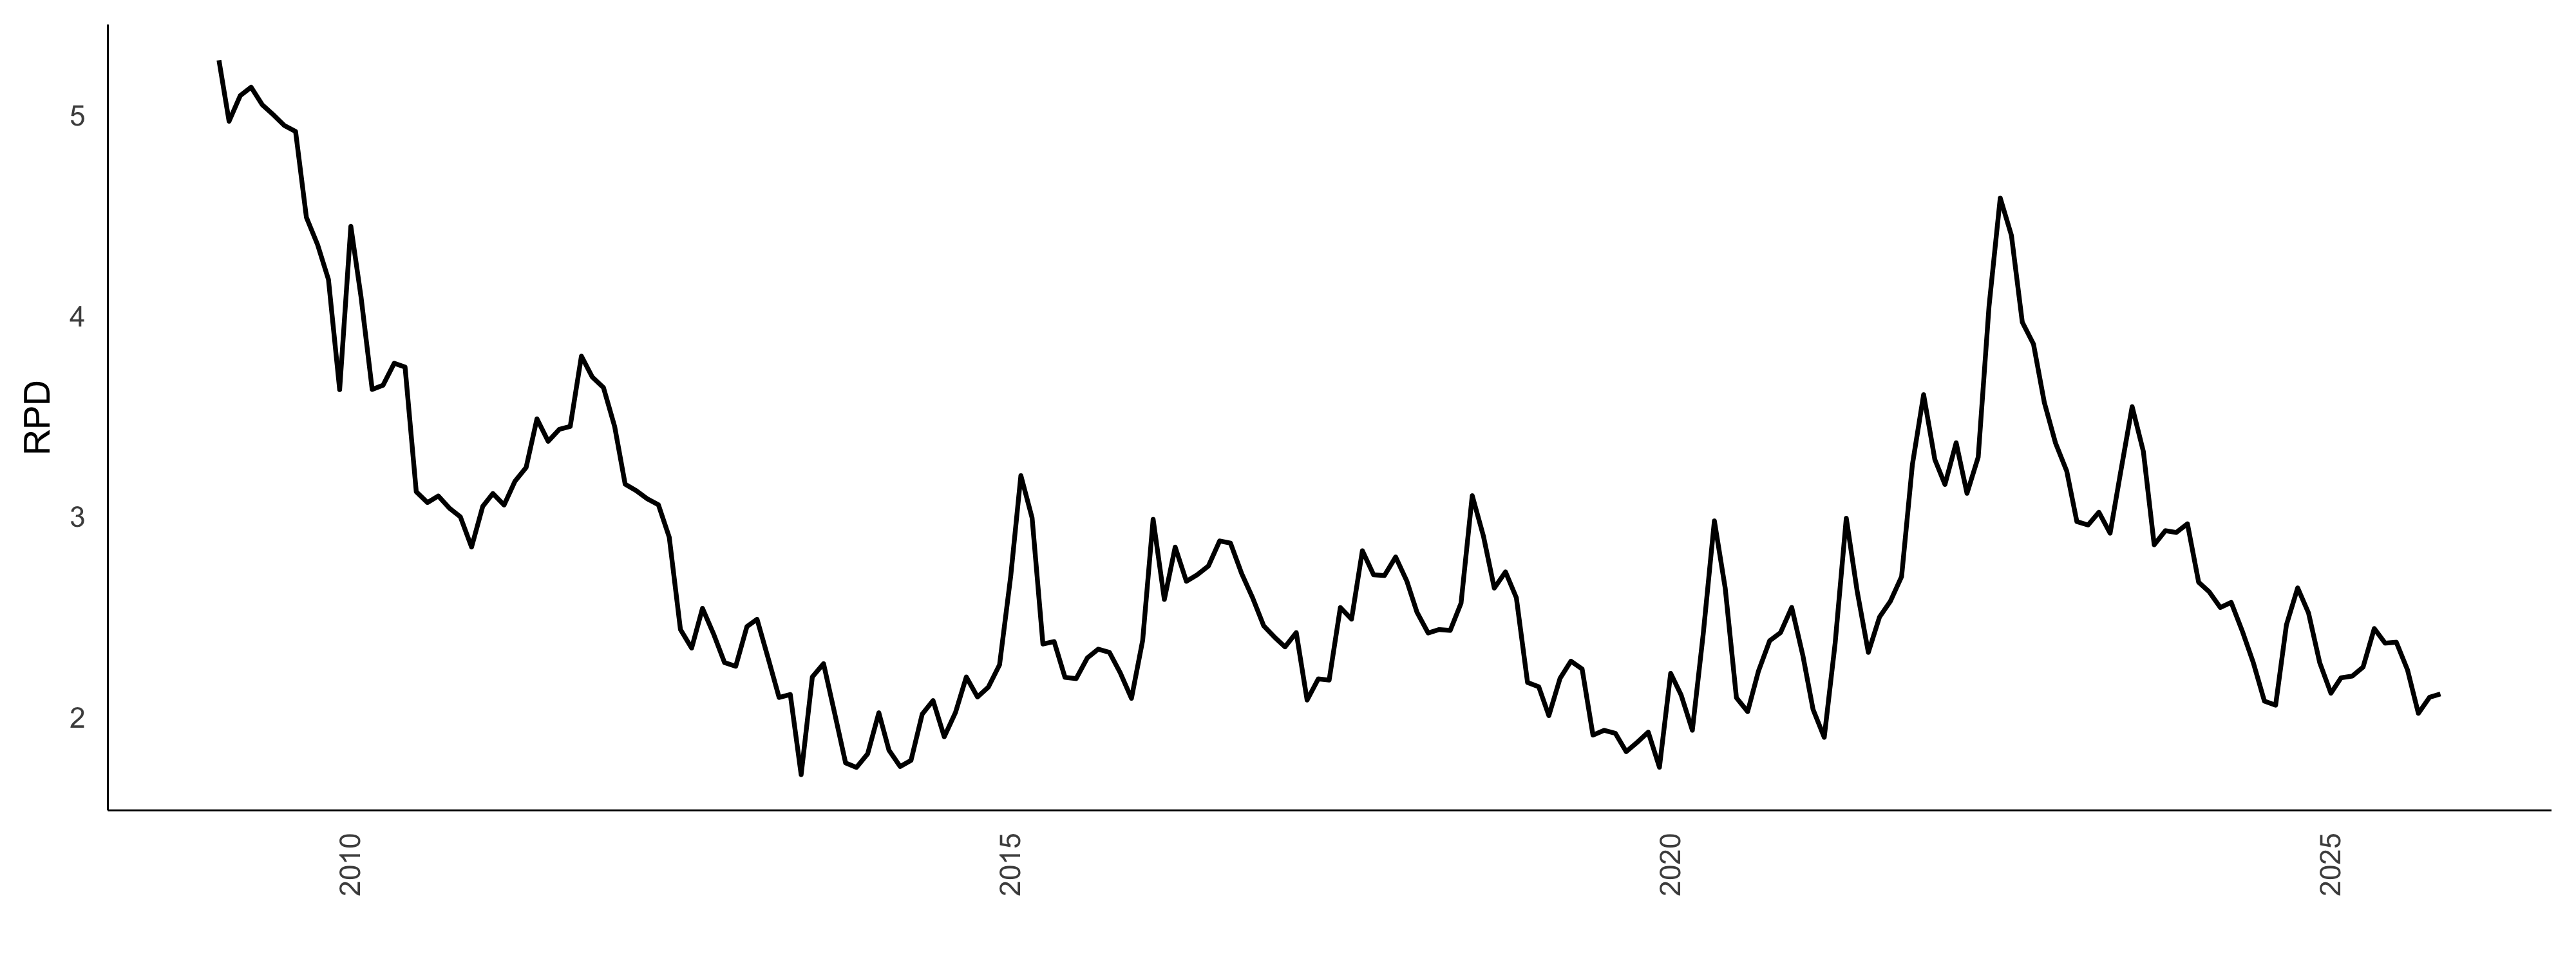
\includegraphics{inflation_relative_price_variance_files/figure-pdf/fig-rpd-1.png}

}

\caption{\label{fig-rpd}RPD over-time}

\end{figure}%

\begin{figure}[H]

\centering{


\includegraphics{inflation_relative_price_variance_files/figure-pdf/fig-rpd_inflation-1.png}

}

\caption{\label{fig-rpd_inflation}RPD vs Headline Inflation. Note: A
quadratic polynomial was fitted on two the data before and after July
2017. This is the period of the first inflation target reform to a
mid-point of 4.5 per cent.}

\end{figure}%

\newpage

The formal estimation in Table~\ref{tbl-base_regression}, using ordinary
least squares of both the linear and quadratic specifications, reveals
that indeed the evidence for non-linearity is stronger. In particular
all the estimates of the quadratic term (\(\pi^2\)) are all significant.
As noted in the methodology section, this significance is in the
presence of estimated break-points in the inflation data. Therefore, the
next question is whether the estimates of the RPD are stable overtime,
or are subject to significant shocks?

\global\setlength{\Oldarrayrulewidth}{\arrayrulewidth}

\global\setlength{\Oldtabcolsep}{\tabcolsep}

\setlength{\tabcolsep}{2pt}

\renewcommand*{\arraystretch}{0.6}



\providecommand{\ascline}[3]{\noalign{\global\arrayrulewidth #1}\arrayrulecolor[HTML]{#2}\cline{#3}}

\begin{longtable}[l]{ccccccc}

\caption{\label{tbl-base_regression}Baseline regressions}

\tabularnewline

\ascline{1pt}{000000}{1-7}

\multicolumn{1}{!{\color[HTML]{FFFFFF}\vrule width 1pt}>{}l}{\textcolor[HTML]{000000}{\fontsize{7}{7}\selectfont{\global\setmainfont{Arial}{\ }}}} & \multicolumn{1}{!{\color[HTML]{FFFFFF}\vrule width 1pt}>{}c}{\textcolor[HTML]{000000}{\fontsize{7}{7}\selectfont{\global\setmainfont{Arial}{Full\ Sample}}}} & \multicolumn{1}{!{\color[HTML]{FFFFFF}\vrule width 1pt}>{}c}{\textcolor[HTML]{000000}{\fontsize{7}{7}\selectfont{\global\setmainfont{Arial}{Pre\ 2017}}}} & \multicolumn{1}{!{\color[HTML]{FFFFFF}\vrule width 1pt}>{}c}{\textcolor[HTML]{000000}{\fontsize{7}{7}\selectfont{\global\setmainfont{Arial}{Post\ 2017}}}} & \multicolumn{1}{!{\color[HTML]{FFFFFF}\vrule width 1pt}>{}c}{\textcolor[HTML]{000000}{\fontsize{7}{7}\selectfont{\global\setmainfont{Arial}{Full\ Sample:\ Squared\ Inflation}}}} & \multicolumn{1}{!{\color[HTML]{FFFFFF}\vrule width 1pt}>{}c}{\textcolor[HTML]{000000}{\fontsize{7}{7}\selectfont{\global\setmainfont{Arial}{Pre\ 2017:\ Squared\ Inflation}}}} & \multicolumn{1}{!{\color[HTML]{FFFFFF}\vrule width 1pt}>{}c!{\color[HTML]{FFFFFF}\vrule width 1pt}}{\textcolor[HTML]{000000}{\fontsize{7}{7}\selectfont{\global\setmainfont{Arial}{Post\ 2017:\ Squared\ Inflation}}}} \\

\ascline{1pt}{000000}{1-7}\endfirsthead 

\ascline{1pt}{000000}{1-7}

\multicolumn{1}{!{\color[HTML]{FFFFFF}\vrule width 1pt}>{}l}{\textcolor[HTML]{000000}{\fontsize{7}{7}\selectfont{\global\setmainfont{Arial}{\ }}}} & \multicolumn{1}{!{\color[HTML]{FFFFFF}\vrule width 1pt}>{}c}{\textcolor[HTML]{000000}{\fontsize{7}{7}\selectfont{\global\setmainfont{Arial}{Full\ Sample}}}} & \multicolumn{1}{!{\color[HTML]{FFFFFF}\vrule width 1pt}>{}c}{\textcolor[HTML]{000000}{\fontsize{7}{7}\selectfont{\global\setmainfont{Arial}{Pre\ 2017}}}} & \multicolumn{1}{!{\color[HTML]{FFFFFF}\vrule width 1pt}>{}c}{\textcolor[HTML]{000000}{\fontsize{7}{7}\selectfont{\global\setmainfont{Arial}{Post\ 2017}}}} & \multicolumn{1}{!{\color[HTML]{FFFFFF}\vrule width 1pt}>{}c}{\textcolor[HTML]{000000}{\fontsize{7}{7}\selectfont{\global\setmainfont{Arial}{Full\ Sample:\ Squared\ Inflation}}}} & \multicolumn{1}{!{\color[HTML]{FFFFFF}\vrule width 1pt}>{}c}{\textcolor[HTML]{000000}{\fontsize{7}{7}\selectfont{\global\setmainfont{Arial}{Pre\ 2017:\ Squared\ Inflation}}}} & \multicolumn{1}{!{\color[HTML]{FFFFFF}\vrule width 1pt}>{}c!{\color[HTML]{FFFFFF}\vrule width 1pt}}{\textcolor[HTML]{000000}{\fontsize{7}{7}\selectfont{\global\setmainfont{Arial}{Post\ 2017:\ Squared\ Inflation}}}} \\

\ascline{1pt}{000000}{1-7}\endhead



\multicolumn{7}{>{}l}{\textcolor[HTML]{000000}{\fontsize{7}{7}\selectfont{\global\setmainfont{Arial}{Note:\ ***\ =\ p\ value\ <\ 0.01,\ **\ =\ 0.01\ <\ p\ value\ <\ 0.05,\ *\ =\ 0.05\ <\ p\ value\ <\ 0.1.}}}} \\

\endlastfoot



\multicolumn{1}{!{\color[HTML]{FFFFFF}\vrule width 1pt}>{}l}{\textcolor[HTML]{000000}{\fontsize{7}{7}\selectfont{\global\setmainfont{Arial}{$\pi_t$}}}} & \multicolumn{1}{!{\color[HTML]{FFFFFF}\vrule width 1pt}>{}c}{\textcolor[HTML]{000000}{\fontsize{7}{7}\selectfont{\global\setmainfont{Arial}{0.01*}}}} & \multicolumn{1}{!{\color[HTML]{FFFFFF}\vrule width 1pt}>{}c}{\textcolor[HTML]{000000}{\fontsize{7}{7}\selectfont{\global\setmainfont{Arial}{0.009\ }}}} & \multicolumn{1}{!{\color[HTML]{FFFFFF}\vrule width 1pt}>{}c}{\textcolor[HTML]{000000}{\fontsize{7}{7}\selectfont{\global\setmainfont{Arial}{0.032***}}}} & \multicolumn{1}{!{\color[HTML]{FFFFFF}\vrule width 1pt}>{}c}{\textcolor[HTML]{000000}{\fontsize{7}{7}\selectfont{\global\setmainfont{Arial}{-0.046\ }}}} & \multicolumn{1}{!{\color[HTML]{FFFFFF}\vrule width 1pt}>{}c}{\textcolor[HTML]{000000}{\fontsize{7}{7}\selectfont{\global\setmainfont{Arial}{-0.104\ }}}} & \multicolumn{1}{!{\color[HTML]{FFFFFF}\vrule width 1pt}>{}c!{\color[HTML]{FFFFFF}\vrule width 1pt}}{\textcolor[HTML]{000000}{\fontsize{7}{7}\selectfont{\global\setmainfont{Arial}{-0.033\ }}}} \\

\ascline{1pt}{FFFFFF}{1-7}



\multicolumn{1}{!{\color[HTML]{FFFFFF}\vrule width 1pt}>{}l}{\textcolor[HTML]{000000}{\fontsize{7}{7}\selectfont{\global\setmainfont{Arial}{$\pi_t^2$}}}} & \multicolumn{1}{!{\color[HTML]{FFFFFF}\vrule width 1pt}>{}c}{\textcolor[HTML]{000000}{\fontsize{7}{7}\selectfont{\global\setmainfont{Arial}{}}}} & \multicolumn{1}{!{\color[HTML]{FFFFFF}\vrule width 1pt}>{}c}{\textcolor[HTML]{000000}{\fontsize{7}{7}\selectfont{\global\setmainfont{Arial}{}}}} & \multicolumn{1}{!{\color[HTML]{FFFFFF}\vrule width 1pt}>{}c}{\textcolor[HTML]{000000}{\fontsize{7}{7}\selectfont{\global\setmainfont{Arial}{}}}} & \multicolumn{1}{!{\color[HTML]{FFFFFF}\vrule width 1pt}>{}c}{\textcolor[HTML]{000000}{\fontsize{7}{7}\selectfont{\global\setmainfont{Arial}{0.006*}}}} & \multicolumn{1}{!{\color[HTML]{FFFFFF}\vrule width 1pt}>{}c}{\textcolor[HTML]{000000}{\fontsize{7}{7}\selectfont{\global\setmainfont{Arial}{0.011*}}}} & \multicolumn{1}{!{\color[HTML]{FFFFFF}\vrule width 1pt}>{}c!{\color[HTML]{FFFFFF}\vrule width 1pt}}{\textcolor[HTML]{000000}{\fontsize{7}{7}\selectfont{\global\setmainfont{Arial}{0.007*}}}} \\

\ascline{1pt}{FFFFFF}{1-7}



\multicolumn{1}{!{\color[HTML]{FFFFFF}\vrule width 1pt}>{}l}{\textcolor[HTML]{000000}{\fontsize{7}{7}\selectfont{\global\setmainfont{Arial}{$RPD_{t-3}$}}}} & \multicolumn{1}{!{\color[HTML]{FFFFFF}\vrule width 1pt}>{}c}{\textcolor[HTML]{000000}{\fontsize{7}{7}\selectfont{\global\setmainfont{Arial}{0.244***}}}} & \multicolumn{1}{!{\color[HTML]{FFFFFF}\vrule width 1pt}>{}c}{\textcolor[HTML]{000000}{\fontsize{7}{7}\selectfont{\global\setmainfont{Arial}{0.173*}}}} & \multicolumn{1}{!{\color[HTML]{FFFFFF}\vrule width 1pt}>{}c}{\textcolor[HTML]{000000}{\fontsize{7}{7}\selectfont{\global\setmainfont{Arial}{0.248**}}}} & \multicolumn{1}{!{\color[HTML]{FFFFFF}\vrule width 1pt}>{}c}{\textcolor[HTML]{000000}{\fontsize{7}{7}\selectfont{\global\setmainfont{Arial}{0.234***}}}} & \multicolumn{1}{!{\color[HTML]{FFFFFF}\vrule width 1pt}>{}c}{\textcolor[HTML]{000000}{\fontsize{7}{7}\selectfont{\global\setmainfont{Arial}{0.154\ }}}} & \multicolumn{1}{!{\color[HTML]{FFFFFF}\vrule width 1pt}>{}c!{\color[HTML]{FFFFFF}\vrule width 1pt}}{\textcolor[HTML]{000000}{\fontsize{7}{7}\selectfont{\global\setmainfont{Arial}{0.209**}}}} \\

\ascline{1pt}{FFFFFF}{1-7}



\multicolumn{1}{!{\color[HTML]{FFFFFF}\vrule width 1pt}>{}l}{\textcolor[HTML]{000000}{\fontsize{7}{7}\selectfont{\global\setmainfont{Arial}{$RPD_{t-2}$}}}} & \multicolumn{1}{!{\color[HTML]{FFFFFF}\vrule width 1pt}>{}c}{\textcolor[HTML]{000000}{\fontsize{7}{7}\selectfont{\global\setmainfont{Arial}{-0.382***}}}} & \multicolumn{1}{!{\color[HTML]{FFFFFF}\vrule width 1pt}>{}c}{\textcolor[HTML]{000000}{\fontsize{7}{7}\selectfont{\global\setmainfont{Arial}{-0.14\ }}}} & \multicolumn{1}{!{\color[HTML]{FFFFFF}\vrule width 1pt}>{}c}{\textcolor[HTML]{000000}{\fontsize{7}{7}\selectfont{\global\setmainfont{Arial}{-0.645***}}}} & \multicolumn{1}{!{\color[HTML]{FFFFFF}\vrule width 1pt}>{}c}{\textcolor[HTML]{000000}{\fontsize{7}{7}\selectfont{\global\setmainfont{Arial}{-0.363***}}}} & \multicolumn{1}{!{\color[HTML]{FFFFFF}\vrule width 1pt}>{}c}{\textcolor[HTML]{000000}{\fontsize{7}{7}\selectfont{\global\setmainfont{Arial}{-0.111\ }}}} & \multicolumn{1}{!{\color[HTML]{FFFFFF}\vrule width 1pt}>{}c!{\color[HTML]{FFFFFF}\vrule width 1pt}}{\textcolor[HTML]{000000}{\fontsize{7}{7}\selectfont{\global\setmainfont{Arial}{-0.609***}}}} \\

\ascline{1pt}{FFFFFF}{1-7}



\multicolumn{1}{!{\color[HTML]{FFFFFF}\vrule width 1pt}>{}l}{\textcolor[HTML]{000000}{\fontsize{7}{7}\selectfont{\global\setmainfont{Arial}{$RPD_{t-1}$}}}} & \multicolumn{1}{!{\color[HTML]{FFFFFF}\vrule width 1pt}>{}c}{\textcolor[HTML]{000000}{\fontsize{7}{7}\selectfont{\global\setmainfont{Arial}{1.039***}}}} & \multicolumn{1}{!{\color[HTML]{FFFFFF}\vrule width 1pt}>{}c}{\textcolor[HTML]{000000}{\fontsize{7}{7}\selectfont{\global\setmainfont{Arial}{0.896***}}}} & \multicolumn{1}{!{\color[HTML]{FFFFFF}\vrule width 1pt}>{}c}{\textcolor[HTML]{000000}{\fontsize{7}{7}\selectfont{\global\setmainfont{Arial}{1.116***}}}} & \multicolumn{1}{!{\color[HTML]{FFFFFF}\vrule width 1pt}>{}c}{\textcolor[HTML]{000000}{\fontsize{7}{7}\selectfont{\global\setmainfont{Arial}{1.017***}}}} & \multicolumn{1}{!{\color[HTML]{FFFFFF}\vrule width 1pt}>{}c}{\textcolor[HTML]{000000}{\fontsize{7}{7}\selectfont{\global\setmainfont{Arial}{0.864***}}}} & \multicolumn{1}{!{\color[HTML]{FFFFFF}\vrule width 1pt}>{}c!{\color[HTML]{FFFFFF}\vrule width 1pt}}{\textcolor[HTML]{000000}{\fontsize{7}{7}\selectfont{\global\setmainfont{Arial}{1.063***}}}} \\

\ascline{1pt}{FFFFFF}{1-7}



\multicolumn{1}{!{\color[HTML]{FFFFFF}\vrule width 1pt}>{}l}{\textcolor[HTML]{000000}{\fontsize{7}{7}\selectfont{\global\setmainfont{Arial}{$D_{2022m8}$}}}} & \multicolumn{1}{!{\color[HTML]{FFFFFF}\vrule width 1pt}>{}c}{\textcolor[HTML]{000000}{\fontsize{7}{7}\selectfont{\global\setmainfont{Arial}{0.026\ }}}} & \multicolumn{1}{!{\color[HTML]{FFFFFF}\vrule width 1pt}>{}c}{\textcolor[HTML]{000000}{\fontsize{7}{7}\selectfont{\global\setmainfont{Arial}{}}}} & \multicolumn{1}{!{\color[HTML]{FFFFFF}\vrule width 1pt}>{}c}{\textcolor[HTML]{000000}{\fontsize{7}{7}\selectfont{\global\setmainfont{Arial}{0.024\ }}}} & \multicolumn{1}{!{\color[HTML]{FFFFFF}\vrule width 1pt}>{}c}{\textcolor[HTML]{000000}{\fontsize{7}{7}\selectfont{\global\setmainfont{Arial}{-0.001\ }}}} & \multicolumn{1}{!{\color[HTML]{FFFFFF}\vrule width 1pt}>{}c}{\textcolor[HTML]{000000}{\fontsize{7}{7}\selectfont{\global\setmainfont{Arial}{}}}} & \multicolumn{1}{!{\color[HTML]{FFFFFF}\vrule width 1pt}>{}c!{\color[HTML]{FFFFFF}\vrule width 1pt}}{\textcolor[HTML]{000000}{\fontsize{7}{7}\selectfont{\global\setmainfont{Arial}{-0.012\ }}}} \\

\ascline{1pt}{FFFFFF}{1-7}



\multicolumn{1}{!{\color[HTML]{FFFFFF}\vrule width 1pt}>{}l}{\textcolor[HTML]{000000}{\fontsize{7}{7}\selectfont{\global\setmainfont{Arial}{$D_{2020m2}$}}}} & \multicolumn{1}{!{\color[HTML]{FFFFFF}\vrule width 1pt}>{}c}{\textcolor[HTML]{000000}{\fontsize{7}{7}\selectfont{\global\setmainfont{Arial}{-0.116\ }}}} & \multicolumn{1}{!{\color[HTML]{FFFFFF}\vrule width 1pt}>{}c}{\textcolor[HTML]{000000}{\fontsize{7}{7}\selectfont{\global\setmainfont{Arial}{}}}} & \multicolumn{1}{!{\color[HTML]{FFFFFF}\vrule width 1pt}>{}c}{\textcolor[HTML]{000000}{\fontsize{7}{7}\selectfont{\global\setmainfont{Arial}{-0.213**}}}} & \multicolumn{1}{!{\color[HTML]{FFFFFF}\vrule width 1pt}>{}c}{\textcolor[HTML]{000000}{\fontsize{7}{7}\selectfont{\global\setmainfont{Arial}{-0.106\ }}}} & \multicolumn{1}{!{\color[HTML]{FFFFFF}\vrule width 1pt}>{}c}{\textcolor[HTML]{000000}{\fontsize{7}{7}\selectfont{\global\setmainfont{Arial}{}}}} & \multicolumn{1}{!{\color[HTML]{FFFFFF}\vrule width 1pt}>{}c!{\color[HTML]{FFFFFF}\vrule width 1pt}}{\textcolor[HTML]{000000}{\fontsize{7}{7}\selectfont{\global\setmainfont{Arial}{-0.205**}}}} \\

\ascline{1pt}{FFFFFF}{1-7}



\multicolumn{1}{!{\color[HTML]{FFFFFF}\vrule width 1pt}>{}l}{\textcolor[HTML]{000000}{\fontsize{7}{7}\selectfont{\global\setmainfont{Arial}{$D_{2017m7}$}}}} & \multicolumn{1}{!{\color[HTML]{FFFFFF}\vrule width 1pt}>{}c}{\textcolor[HTML]{000000}{\fontsize{7}{7}\selectfont{\global\setmainfont{Arial}{0.156*}}}} & \multicolumn{1}{!{\color[HTML]{FFFFFF}\vrule width 1pt}>{}c}{\textcolor[HTML]{000000}{\fontsize{7}{7}\selectfont{\global\setmainfont{Arial}{}}}} & \multicolumn{1}{!{\color[HTML]{FFFFFF}\vrule width 1pt}>{}c}{\textcolor[HTML]{000000}{\fontsize{7}{7}\selectfont{\global\setmainfont{Arial}{}}}} & \multicolumn{1}{!{\color[HTML]{FFFFFF}\vrule width 1pt}>{}c}{\textcolor[HTML]{000000}{\fontsize{7}{7}\selectfont{\global\setmainfont{Arial}{0.161*}}}} & \multicolumn{1}{!{\color[HTML]{FFFFFF}\vrule width 1pt}>{}c}{\textcolor[HTML]{000000}{\fontsize{7}{7}\selectfont{\global\setmainfont{Arial}{}}}} & \multicolumn{1}{!{\color[HTML]{FFFFFF}\vrule width 1pt}>{}c!{\color[HTML]{FFFFFF}\vrule width 1pt}}{\textcolor[HTML]{000000}{\fontsize{7}{7}\selectfont{\global\setmainfont{Arial}{}}}} \\

\ascline{1pt}{FFFFFF}{1-7}



\multicolumn{1}{!{\color[HTML]{FFFFFF}\vrule width 1pt}>{}l}{\textcolor[HTML]{000000}{\fontsize{7}{7}\selectfont{\global\setmainfont{Arial}{$D_{2014m7}$}}}} & \multicolumn{1}{!{\color[HTML]{FFFFFF}\vrule width 1pt}>{}c}{\textcolor[HTML]{000000}{\fontsize{7}{7}\selectfont{\global\setmainfont{Arial}{-0.098\ }}}} & \multicolumn{1}{!{\color[HTML]{FFFFFF}\vrule width 1pt}>{}c}{\textcolor[HTML]{000000}{\fontsize{7}{7}\selectfont{\global\setmainfont{Arial}{-0.087\ }}}} & \multicolumn{1}{!{\color[HTML]{FFFFFF}\vrule width 1pt}>{}c}{\textcolor[HTML]{000000}{\fontsize{7}{7}\selectfont{\global\setmainfont{Arial}{}}}} & \multicolumn{1}{!{\color[HTML]{FFFFFF}\vrule width 1pt}>{}c}{\textcolor[HTML]{000000}{\fontsize{7}{7}\selectfont{\global\setmainfont{Arial}{-0.105\ }}}} & \multicolumn{1}{!{\color[HTML]{FFFFFF}\vrule width 1pt}>{}c}{\textcolor[HTML]{000000}{\fontsize{7}{7}\selectfont{\global\setmainfont{Arial}{-0.096\ }}}} & \multicolumn{1}{!{\color[HTML]{FFFFFF}\vrule width 1pt}>{}c!{\color[HTML]{FFFFFF}\vrule width 1pt}}{\textcolor[HTML]{000000}{\fontsize{7}{7}\selectfont{\global\setmainfont{Arial}{}}}} \\

\ascline{1pt}{FFFFFF}{1-7}



\multicolumn{1}{!{\color[HTML]{FFFFFF}\vrule width 1pt}>{}l}{\textcolor[HTML]{000000}{\fontsize{7}{7}\selectfont{\global\setmainfont{Arial}{$D_{2011m12}$}}}} & \multicolumn{1}{!{\color[HTML]{FFFFFF}\vrule width 1pt}>{}c}{\textcolor[HTML]{000000}{\fontsize{7}{7}\selectfont{\global\setmainfont{Arial}{0.042\ }}}} & \multicolumn{1}{!{\color[HTML]{FFFFFF}\vrule width 1pt}>{}c}{\textcolor[HTML]{000000}{\fontsize{7}{7}\selectfont{\global\setmainfont{Arial}{0.027\ }}}} & \multicolumn{1}{!{\color[HTML]{FFFFFF}\vrule width 1pt}>{}c}{\textcolor[HTML]{000000}{\fontsize{7}{7}\selectfont{\global\setmainfont{Arial}{}}}} & \multicolumn{1}{!{\color[HTML]{FFFFFF}\vrule width 1pt}>{}c}{\textcolor[HTML]{000000}{\fontsize{7}{7}\selectfont{\global\setmainfont{Arial}{0.047\ }}}} & \multicolumn{1}{!{\color[HTML]{FFFFFF}\vrule width 1pt}>{}c}{\textcolor[HTML]{000000}{\fontsize{7}{7}\selectfont{\global\setmainfont{Arial}{0.037\ }}}} & \multicolumn{1}{!{\color[HTML]{FFFFFF}\vrule width 1pt}>{}c!{\color[HTML]{FFFFFF}\vrule width 1pt}}{\textcolor[HTML]{000000}{\fontsize{7}{7}\selectfont{\global\setmainfont{Arial}{}}}} \\

\ascline{1pt}{FFFFFF}{1-7}



\multicolumn{1}{!{\color[HTML]{FFFFFF}\vrule width 1pt}>{}l}{\textcolor[HTML]{000000}{\fontsize{7}{7}\selectfont{\global\setmainfont{Arial}{$C$}}}} & \multicolumn{1}{!{\color[HTML]{FFFFFF}\vrule width 1pt}>{}c}{\textcolor[HTML]{000000}{\fontsize{7}{7}\selectfont{\global\setmainfont{Arial}{0.044\ }}}} & \multicolumn{1}{!{\color[HTML]{FFFFFF}\vrule width 1pt}>{}c}{\textcolor[HTML]{000000}{\fontsize{7}{7}\selectfont{\global\setmainfont{Arial}{0.012\ }}}} & \multicolumn{1}{!{\color[HTML]{FFFFFF}\vrule width 1pt}>{}c}{\textcolor[HTML]{000000}{\fontsize{7}{7}\selectfont{\global\setmainfont{Arial}{0.117***}}}} & \multicolumn{1}{!{\color[HTML]{FFFFFF}\vrule width 1pt}>{}c}{\textcolor[HTML]{000000}{\fontsize{7}{7}\selectfont{\global\setmainfont{Arial}{0.184**}}}} & \multicolumn{1}{!{\color[HTML]{FFFFFF}\vrule width 1pt}>{}c}{\textcolor[HTML]{000000}{\fontsize{7}{7}\selectfont{\global\setmainfont{Arial}{0.326*}}}} & \multicolumn{1}{!{\color[HTML]{FFFFFF}\vrule width 1pt}>{}c!{\color[HTML]{FFFFFF}\vrule width 1pt}}{\textcolor[HTML]{000000}{\fontsize{7}{7}\selectfont{\global\setmainfont{Arial}{0.304**}}}} \\

\ascline{1pt}{000000}{1-7}


\end{longtable}

\arrayrulecolor[HTML]{000000}

\global\setlength{\arrayrulewidth}{\Oldarrayrulewidth}

\global\setlength{\tabcolsep}{\Oldtabcolsep}

\renewcommand*{\arraystretch}{1}

In Figure~\ref{fig-rolling_coefficients} and Figure~\ref{fig-recursive}
we estimate the rolling and recursive estimates. 24 and 60 month windows
are implemented for the rolling window estimation. The results of both
methods suggest a dynamic relationship with periods of strong
significance. In the main, we observe a positive response of RPD to a 1
percentage point change in headline inflation. This dynamic relationship
further builds the case for a U-shaped relationship.

\begin{figure}[H]

\centering{


\includegraphics{inflation_relative_price_variance_files/figure-pdf/fig-rolling_coefficients-1.png}

}

\caption{\label{fig-rolling_coefficients}Rolling regressions. Note:
t-statistics of greater (or less) than 1.96 ( or -1.96) is significant
at a 5\% level of significance.}

\end{figure}%

\begin{figure}[H]

\centering{


\includegraphics{inflation_relative_price_variance_files/figure-pdf/fig-recursive-1.png}

}

\caption{\label{fig-recursive}Recursive regressions. Note: Recursive
regression estimates of the coefficient on absolute headline inflation
with a fixed start date of 2012-07.}

\end{figure}%

\newpage

Figure~\ref{fig-semi_parametric} shows the estimated nonparametric
conditional mean effect of inflation on RPD for the full sample,
pre-2017 and post-2017 samples. The optimal bandwidth was selected
automatically using cross-validation method. To test the sensitivity of
the nonparametric estimates to the smoothing parameter, we also consider
smaller and larger bandwidths in both Figure~\ref{fig-semi_parametric}
and Figure~\ref{fig-unexpected_inflation}, in both cases the results are
qualitatively similar indicating that the nonparametric estimates are
robust to the smoothing parameter. In Figure~\ref{fig-semi_parametric}
across all samples, the relationship is approximately linear and upward
sloping indicating that the marginal effect is positive across the
inflation range, broadly in line with the menu cost theoretical
predictions.

Specifically, in the full sample, Figure~\ref{fig-semi_parametric} shows
that small positive effects on RPD for the inflation range of 2-3 per
cent, with RPD is at its lowest in this range suggesting that the
optimal inflation lies within this range as RPD is not amplified,
otherwise RPD increases monotonically as inflation increases beyond this
range. Thus, higher average inflation increases price misconception,
leading to inefficient resource allocation equivalent to a negative
productivity shock \citep{damjanovic2010}. The pre-2017 sample results
show a similar profile except that a 3 per cent inflation rate minimises
price dispersion. These findings are similar across both the Gaussian
and Epanechnikov kernels.

Interestingly, the sub-samples results show regime shifts in the
inflation and RPD relationship. The post-2017 sub-sample still shows
positive and linear effects however the curvature is weaker and flatter
in contrast to the pre-2017 period, which shows evidence of
regime-dependence \citep{choi2011, baglan2016, hornstein2024}.
Specifically, relatively lower regimes levels are associated with weaker
inflation effects on RPD because even at high inflation rates in the
range of 7-8 per cent the curve is less steep than pre-2017 results -
suggesting a less responsive RPD. The results in
Figure~\ref{fig-semi_parametric} suggest the optimal inflation rate in
the post-2017 sub-sample is also in the range of 2-3 per cent. These
optimal inflation rate estimates are lower than the 4 per cent estimate
from \citep{caraballo2013} whom we closely follow in our empirical
framework but our results are closer to estimates in the literature. See
\citet{diercks2019} for a summary of these studies.\footnote{Menu cost
  models generally find the optimal inflation rate to be 0 per cent and
  studies that take into account the zero-lower bound constraint,
  measurement bias in inflation measure and downward wage rigidities
  generally propose an optimal inflation rate that are positive at near
  2 per cent}

\newpage

\begin{figure}[H]

\centering{


\includegraphics{inflation_relative_price_variance_files/figure-pdf/fig-semi_parametric-1.png}

}

\caption{\label{fig-semi_parametric}Semi-parametric regressions for
headline inflation. Note: hcpi is headline inflation. This figure shows
the estimated nonparametric conditional mean effect of headline
inflation on RPD for the full sample, pre-2017 and post-2017 samples.
The optimal bandwidth was selected automatically using cross-validation
method.}

\end{figure}%

\newpage

\begin{figure}[H]

\centering{


\includegraphics{inflation_relative_price_variance_files/figure-pdf/fig-unexpected_inflation-1.png}

}

\caption{\label{fig-unexpected_inflation}Semi-parametric regressions for
unexpected inflation. Note: hcpi\_u is the unexpected component of
headline inflation. This figure shows the estimated nonparametric
conditional mean effect of unexpected inflation on RPD for the full
sample, pre-2017 and post-2017 samples. The optimal bandwidth was
selected automatically using cross-validation method.}

\end{figure}%

Figure~\ref{fig-unexpected_inflation} shows the estimated results of the
nonparametric effect of unexpected inflation on RPD and the findings are
broadly consistent with the predictions of the signal extraction theory.
These results exhibit a U-shaped profile. Positive and negative
surprises both increase relative price variability however the effects
are asymmetric. Positive inflation surprises generate a stronger
dispersion response than negative ones.

Notably, the estimated effects are similar in both the full sample and
the pre-2017 sample periods. The response of RPD to negative inflation
surprises is relatively moderate and relatively flat, while positive
inflation causes RPD to accelerate more noticeably particularly for
inflation surprises near 0.2 and above. This suggests that price-setters
respond more aggressively to inflationary surprises than deflationary
ones suggesting that positive inflation surprises create informational
noise and as a result firms confuse aggregate price shocks with relative
shocks leading to higher relative price variability consistent with the
misconception models. However unlike these theoretical predictions as
well as the empirical studies
\citep{caraballo2013, becker2012, sara-zaror2024} the positive and
negative inflation shocks, in our case, do not have a symmetric effect
on RPD. The post-2017 suggests a structural regime change in the
relationship as the magnitude of the effect of unexpected inflation on
RPD is weaker on either side of the distribution. We attribute this to a
relatively low inflation regime as well as better anchored inflation
expectations \citep{durand2023} in the post-2017 period in line with the
adoption of a lower inflation targets in both 2017 as well as 2025. For
example, the x-axis only extends to about ±0.25 percentage points in the
post-2017 sample, reflecting less variation in unexpected inflation
compared to the pre-2017 sample. Furthermore, the latter years in our
sample are characterised by significant global shocks to inflation from
the COVID-2019 Pandemic in 2020, the post-pandemic recovery induced
energy price shock in 2021 as well as the global food price shock after
the outbreak of the Russia-Ukraine war in 2022. These global shocks
would've induced a similar price setting behavioural response in the
same direction therefore compressing price dispersion
\citep{nakamura2018} which, in our view, also explains the relatively
benign results post-2017.

\section{Robustness}\label{robustness}

To further investigate the idea of RPD-inflation regimes, we take a
novel approach in the literature to estimate a quantile-on-quantile
(QQR) regression analysis \citep{koenker2017}. The QQR will further
examine the inflation-RPD nexus since kernel estimation in
Figure~\ref{fig-semi_parametric} and
Figure~\ref{fig-unexpected_inflation} show average marginal effects
across the inflation distribution, while the QQR directly estimates the
dependence structure across the joint distribution of inflation
(\(\tau\)) and RPD (\(\theta\)). The results in
Figure~\ref{fig-quant_reg} show that, across the all sub-samples, in
most quantiles of RPD, higher quantiles of inflation are associated with
a positive and increasingly strong effect on RPD. When inflation is in
its upper quantiles (\(\tau \rightarrow 1\)), the coefficient is at its
largest and most positive, suggesting a strong amplification where high
inflation episodes are associated with meaningfully larger relative
price dispersion. At low quantiles of inflation (\(\tau \leftarrow 0\)),
the relationship is substantially muted and largely statistically
insignificant (white areas), particularly for middle quantiles of RPD
indicating that low or stable inflation has little systematic effect on
relative price dispersion. This is a double confirmation of the U-shaped
relationship. Furthermore, lower quantiles of RPD (\(\theta < 0.25\))
show weak effects throughout, implying that episodes of low-price
dispersion are relatively insensitive to inflation regardless of where
inflation sits in its distribution.

Notably in the post-2017 sub-sample, structural changes in the
relationship are evident. Firstly, the size of the magnitude is larger
and the positive effects are concentrated at very high inflation
quantiles likely reflecting the heightened inflationary volatility of
the post-2017 period, including commodity price shocks and the COVID-19
era inflation surge. Secondly, there is a wider region of insignificance
at low and mid inflation quantiles (\(\tau < 0.50\)) particularly for
lower quantiles of RPD implying low-to-moderate inflation in the
post-2017 associated with reductions in the inflation target, has little
systematic effect on price dispersion. The relationship being driven
almost entirely by tail inflation events or shocks.

\begin{figure}[H]

\centering{

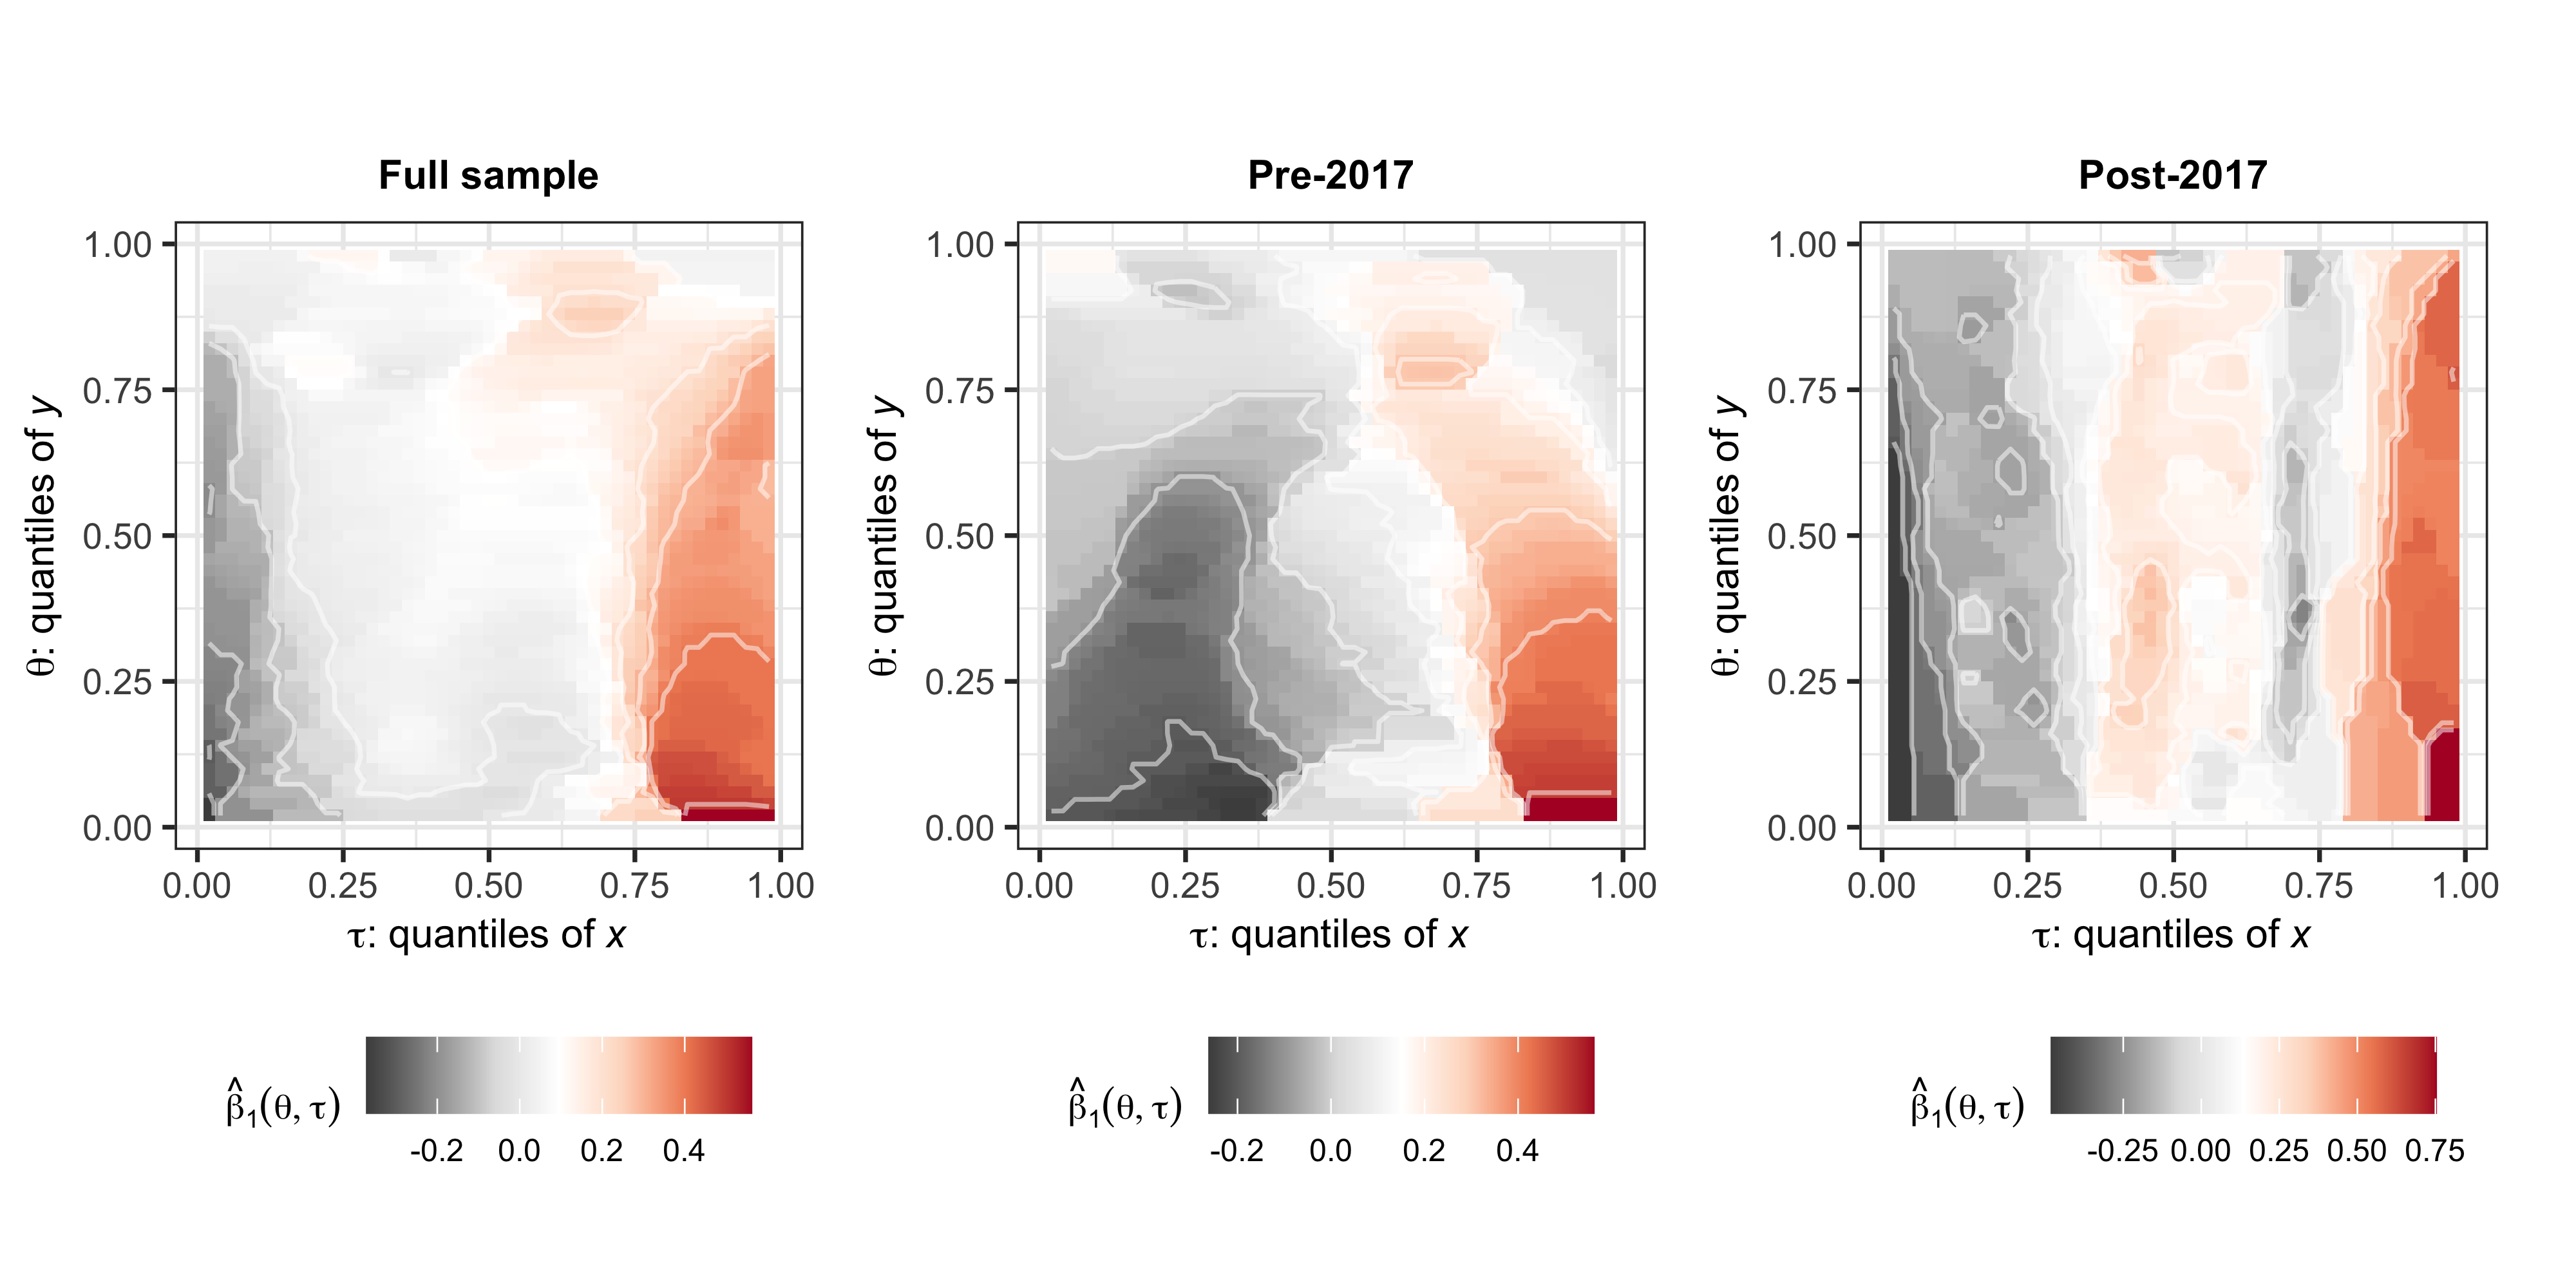
\includegraphics{inflation_relative_price_variance_files/figure-pdf/fig-quant_reg-1.png}

}

\caption{\label{fig-quant_reg}Quantile on quantile regressions for
headline inflation. Note: In the quantile on quatile regression plots,
the x-axis represents the quantiles of headline inflation, while the
y-axis represents the quantiles of RPD. The color gradient indicates the
strength and direction of the relationship between headline inflation
and RPD across different quantiles. Warmer colors (e.g., red) indicate a
stronger positive relationship, while cooler colors (e.g., blue)
indicate a stronger negative relationship. The white areas represent
quantiles where the relationship is not statistically significant.}

\end{figure}%

Interestingly the positive coefficient region in
Figure~\ref{fig-unif_quant_reg} is larger and more pervasive across the
space compared to Figure~\ref{fig-quant_reg} with the implication that
unexpected inflation appears to have a stronger and more broadly
distributed positive effect on relative price dispersion than aggregate
inflation. Specifically, positive inflation surprises have a visible
effect on RPD even at moderate quantiles in the pre-2017 era. This
implies that even modest positive inflation surprises - not just extreme
ones - were sufficient to generate significant RPD responses before
2017. The lower quantiles of RPD (\(\theta < 0.25\)) remain largely
insignificant. Interestingly, there is a weak negative region at very
low quantiles of unexpected inflation for mid-range RPD, suggesting that
negative inflation surprises were mildly associated with reduced
dispersion in this era.

Positive inflation surprises have less concentrated effects in the
post-2017 sub-sample compared to the pre-2017 period however the
coefficient scale is wider compared to pre-2017 indicating the
sensitivity of RPD to unexpected inflation as inflation shocks surged
enormously after 2017 and these shocks were more disruptive to relative
price alignment. There is a broader insignificance at intermediate
quantile combinations. A notable feature of the post-2017 sub-sample is
the emergence of statistically significant negative coefficients at low
quantiles of unexpected inflation (\(\tau < 0.25\)), particularly across
mid-to-high quantiles of RPD (\(\theta > 0.25\)). This means negative
inflation surprises in the post-2017 period, were associated with lower
RPD. This pattern was absent (or negligible) pre-2017. We attribute this
to the likelihood that when inflation expectations were managed down by
the central bank as inflation targets are lowered, downside inflation
surprises actively compress price dispersion, while upside surprises
amplify it \citep{bems2021, moessner2020}.

\begin{figure}[H]

\centering{

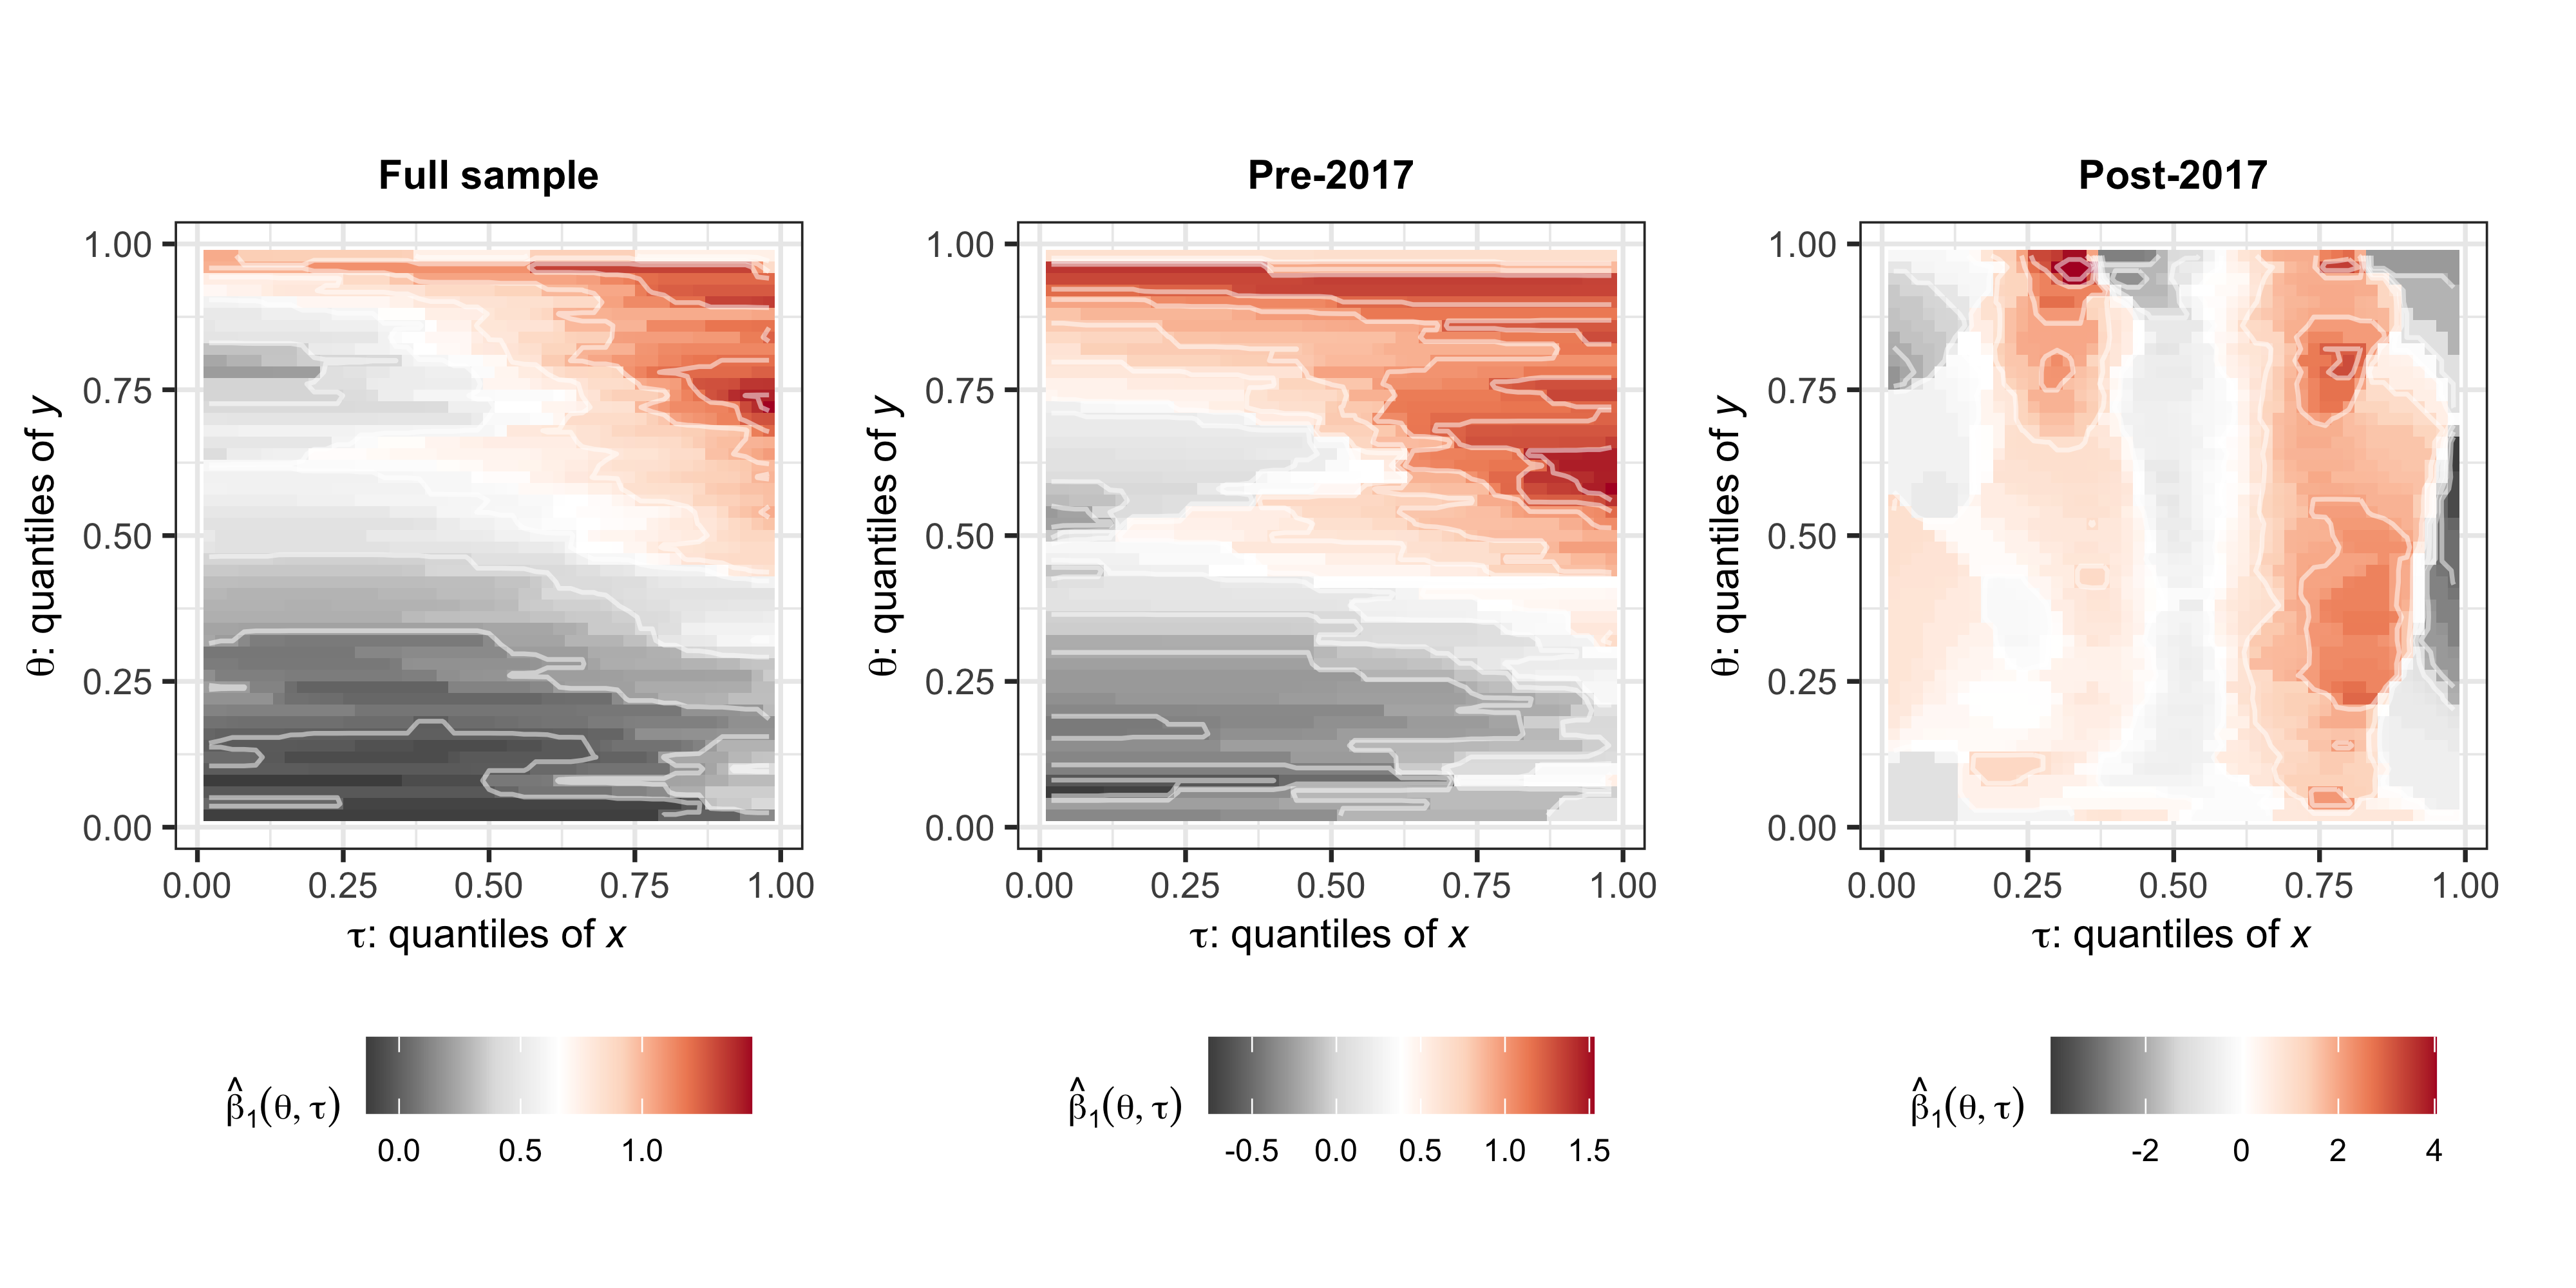
\includegraphics{inflation_relative_price_variance_files/figure-pdf/fig-unif_quant_reg-1.png}

}

\caption{\label{fig-unif_quant_reg}Quantile on quantile regressions for
the unexpected component of inflation. Note: The x-axis represents the
quantiles of the unexpected component of headline inflation, while the
y-axis represents the quantiles of RPD.}

\end{figure}%

\newpage

\section{Conclusion}\label{conclusion}

This paper provides a comprehensive empirical analysis of the
relationship between inflation and relative price dispersion (RPD) in
South Africa, highlighting the importance of structural changes in
inflation targeting on this nexus. Our findings support the presence of
a nonlinear, U-shaped relationship between inflation and RPD, consistent
with the signal extraction and monetary search models that allow for a
non-zero optimal inflation rate. The semi-parametric estimation revealed
that average inflation effects on price dispersion evolve over time,
especially around changes in inflation targets, while the
quantile-on-quantile regression uncovered heterogeneity in the impact of
inflation across different parts of the RPD distribution. This dynamic
behavior reinforces the idea that moderate inflation may not only be
inevitable but could also reduce welfare losses associated with price
rigidities and informational frictions. Interestingly, testing the
predictions of the signal extraction models, inflation surprises in our
case do not have a symmetric effect on price relative variability
instead, only positive surprises worsen price variability or RPD.

The post-2017 period is characterized by a unique combination of factors
including lower-than-expected inflation, a revised lower inflation
target, and significant global shocks such as the COVID-19 pandemic,
supply chain disruptions, energy price shocks, and the Russia-Ukraine
conflict. These elements contributed to synchronized price adjustments
across firms, compressing relative price dispersion and resulting in a
negative, monotonic relationship between unexpected inflation and RPD
during this period. Our results suggest that the inflation-RPD trade-off
may currently be in a transitory phase, moving towards a more favorable
profile compared to the pre-2017 era.

This analysis contributes to the relatively sparse literature on
emerging markets by providing nuanced insights into how inflation
influences relative price variability under evolving monetary policy
frameworks. Moreover, our findings are supportive of the decision to
lower South Africa's inflation target in 2025. The South African
experience---moving from broad inflation bands to more precise target
midpoints and planned reductions in target levels---demonstrates the
complex interplay between inflation regimes and price adjustments.
Policymakers targeting lower inflation in similar emerging economies
should consider these nonlinear dynamics and transitional effects to
strike a balance between inflation control and minimizing distortions in
relative prices that can hinder efficient resource allocation and
economic growth. Ultimately, our results advocate for flexible inflation
targets that account for structural features of the economy and the
benefits of moderate inflation in optimizing welfare. \newpage

\section*{References}\label{references}
\addcontentsline{toc}{section}{References}

\renewcommand{\bibsection}{}
\bibliography{references.bib}

\setcounter{section}{0}
\renewcommand{\thesection}{\Alph{section}}
\setcounter{table}{0}
\renewcommand{\thetable}{A\arabic{table}}
\setcounter{figure}{0}
\renewcommand{\thefigure}{A\arabic{figure}}
\newpage

\section{Appendix: Data and descriptive
statistics}\label{appendix-data-and-descriptive-statistics}

\subsection{Data}\label{data}

\begin{figure}[H]

\centering{


\includegraphics{inflation_relative_price_variance_files/figure-pdf/fig-headline_inflation-1.png}

}

\caption{\label{fig-headline_inflation}Headline inflation (\%).}

\end{figure}%

\begin{figure}[H]

\centering{


\includegraphics{inflation_relative_price_variance_files/figure-pdf/fig-price_data-1.png}

}

\caption{\label{fig-price_data}Inflation categories (\%)}

\end{figure}%

\begin{figure}[H]

\centering{

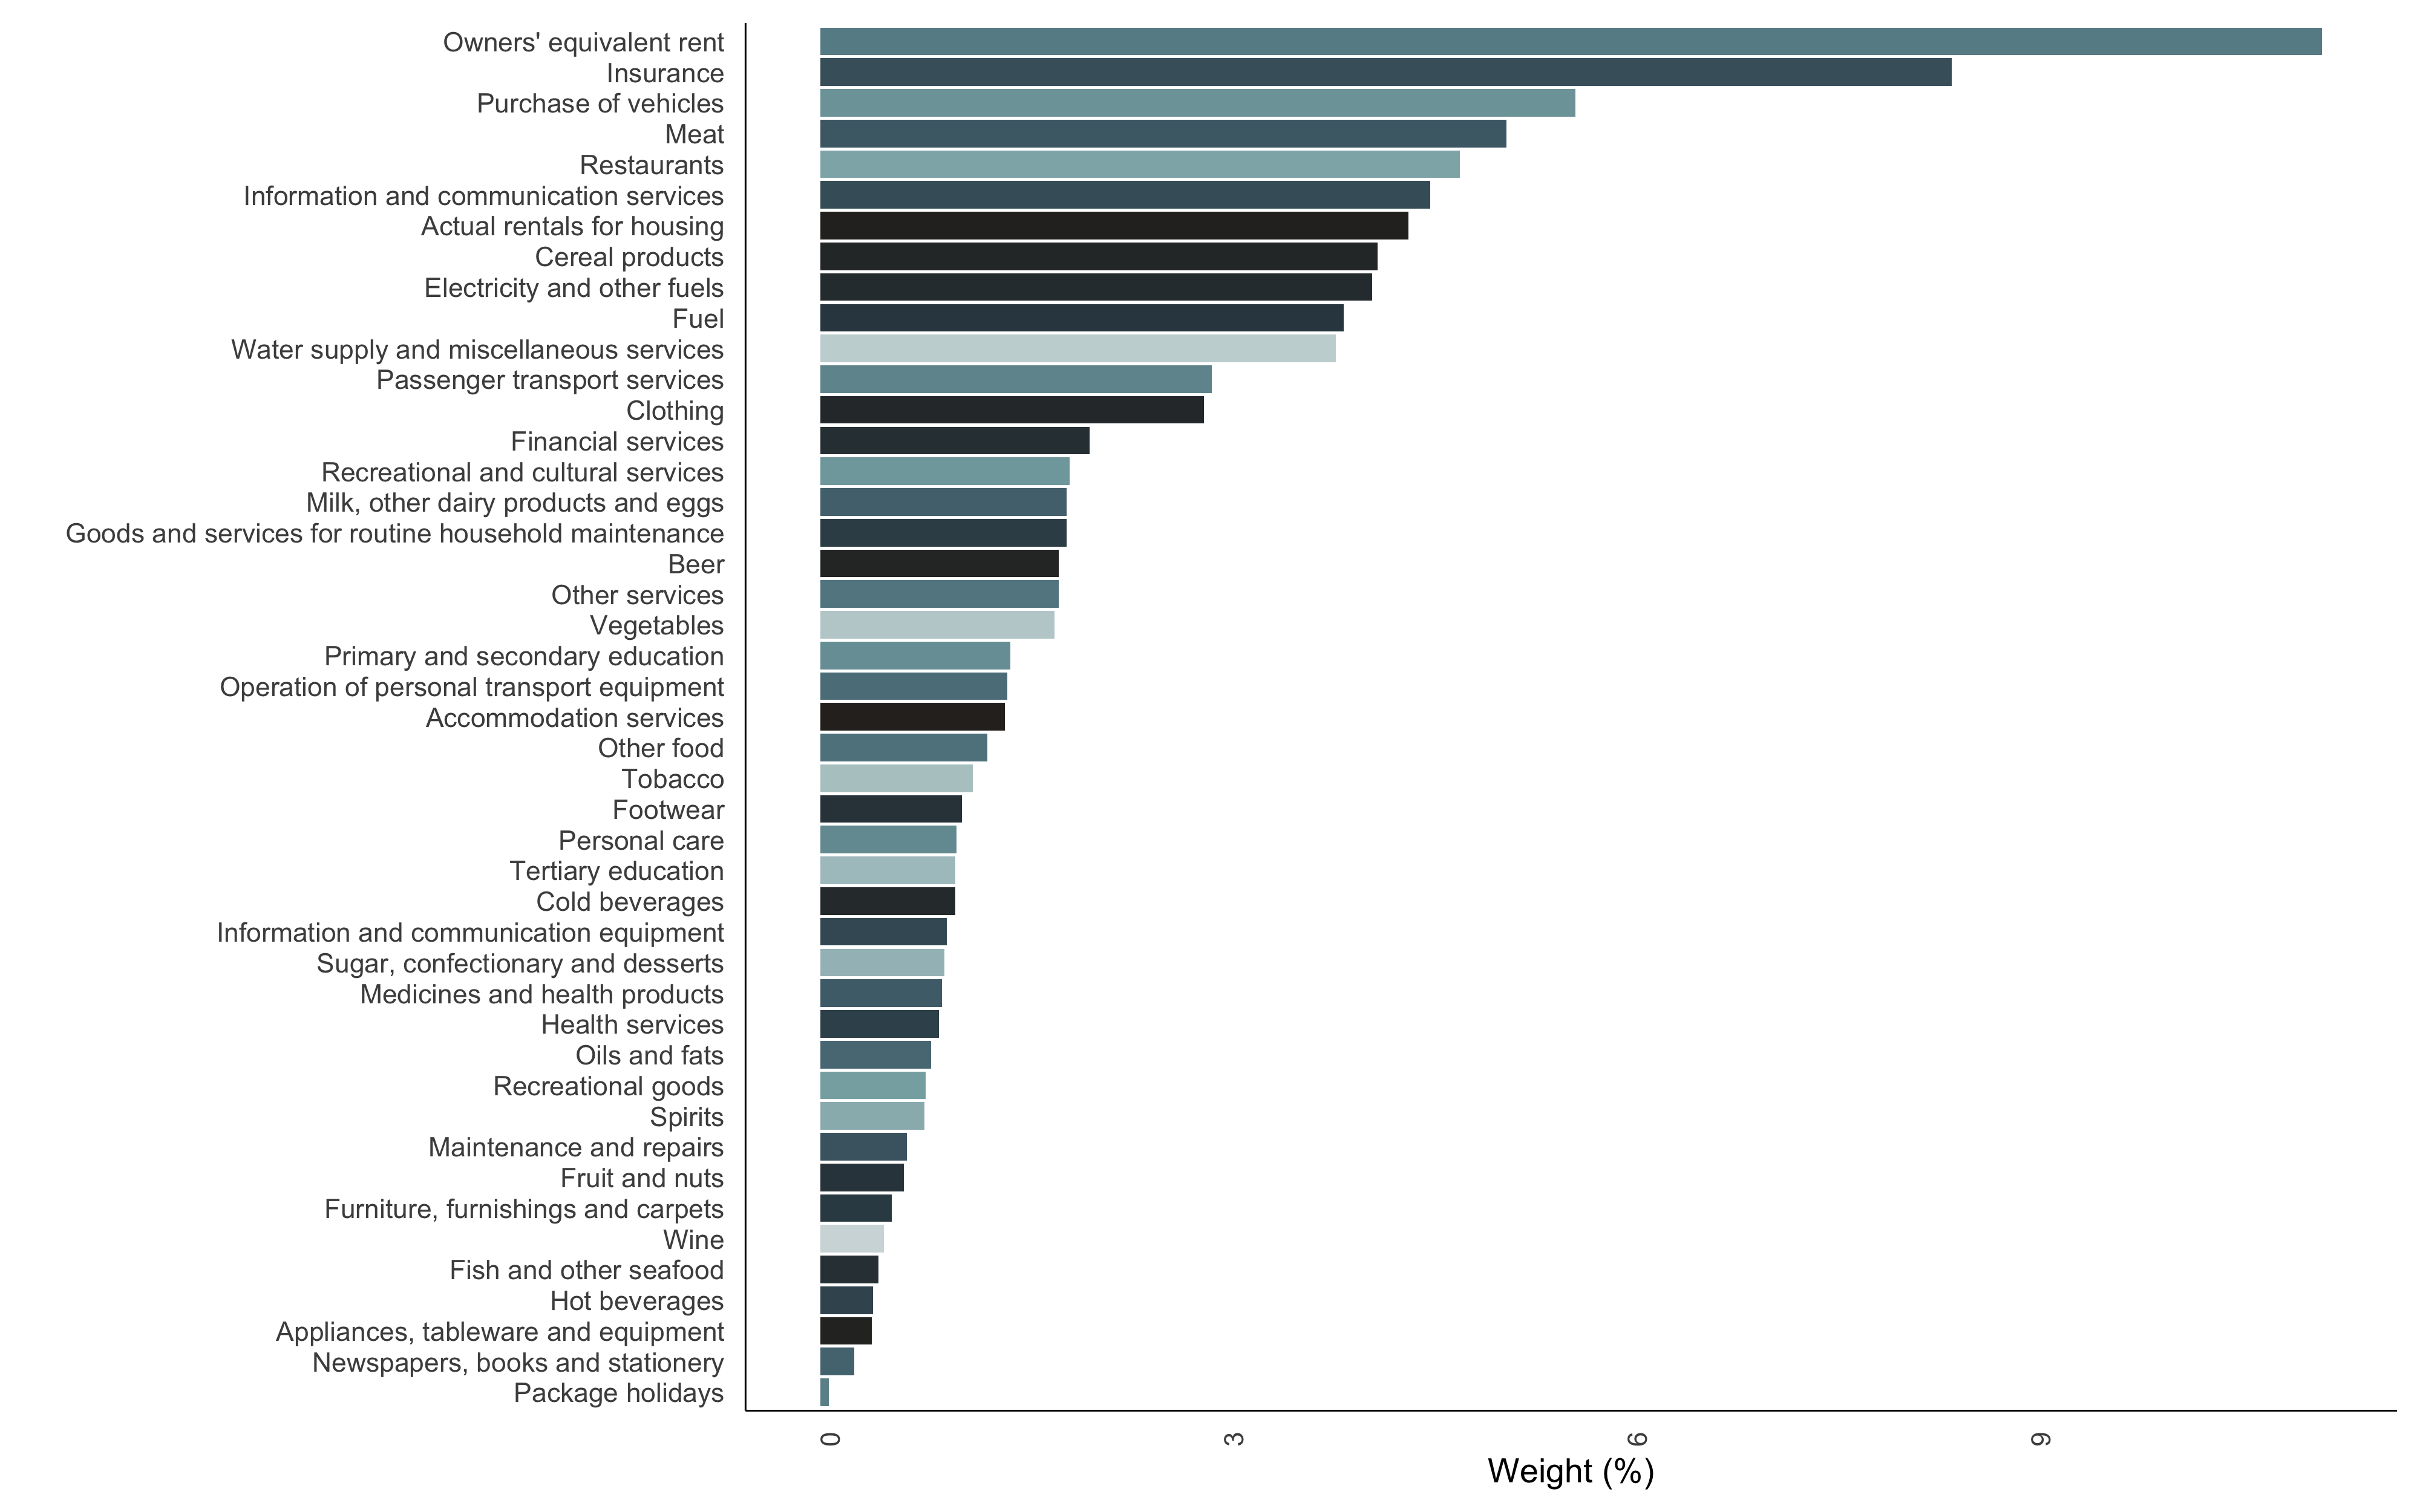
\includegraphics{inflation_relative_price_variance_files/figure-pdf/fig-weights-1.png}

}

\caption{\label{fig-weights}CPI Weights. Note: Due to a lack of data,
some categories (no spitirits; transport services of goods; household
textiles; glassware,tableware, and house utensils; and Tools and
equipment for house and garden) have been excluded.}

\end{figure}%

\newpage

\subsection{Descriptive statistics}\label{descriptive-statistics}

\global\setlength{\Oldarrayrulewidth}{\arrayrulewidth}

\global\setlength{\Oldtabcolsep}{\tabcolsep}

\setlength{\tabcolsep}{2pt}

\renewcommand*{\arraystretch}{0.5}



\providecommand{\ascline}[3]{\noalign{\global\arrayrulewidth #1}\arrayrulecolor[HTML]{#2}\cline{#3}}

\begin{longtable}[l]{|p{2.57in}|p{0.46in}|p{0.50in}|p{0.43in}|p{0.46in}|p{0.43in}|p{0.76in}}

\caption{\label{tbl-descriptive_stats}Descriptive statistics}

\tabularnewline

\ascline{1pt}{000000}{1-7}

\multicolumn{1}{!{\color[HTML]{FFFFFF}\vrule width 1pt}>{\raggedright}m{\dimexpr 2.57in+0\tabcolsep}}{\textcolor[HTML]{000000}{\fontsize{7}{7}\selectfont{\global\setmainfont{Arial}{Variable}}}} & \multicolumn{1}{!{\color[HTML]{FFFFFF}\vrule width 1pt}>{\centering}m{\dimexpr 0.46in+0\tabcolsep}}{\textcolor[HTML]{000000}{\fontsize{7}{7}\selectfont{\global\setmainfont{Arial}{Mean}}}} & \multicolumn{1}{!{\color[HTML]{FFFFFF}\vrule width 1pt}>{\centering}m{\dimexpr 0.5in+0\tabcolsep}}{\textcolor[HTML]{000000}{\fontsize{7}{7}\selectfont{\global\setmainfont{Arial}{Median}}}} & \multicolumn{1}{!{\color[HTML]{FFFFFF}\vrule width 1pt}>{\centering}m{\dimexpr 0.43in+0\tabcolsep}}{\textcolor[HTML]{000000}{\fontsize{7}{7}\selectfont{\global\setmainfont{Arial}{SD}}}} & \multicolumn{1}{!{\color[HTML]{FFFFFF}\vrule width 1pt}>{\centering}m{\dimexpr 0.46in+0\tabcolsep}}{\textcolor[HTML]{000000}{\fontsize{7}{7}\selectfont{\global\setmainfont{Arial}{Min}}}} & \multicolumn{1}{!{\color[HTML]{FFFFFF}\vrule width 1pt}>{\centering}m{\dimexpr 0.43in+0\tabcolsep}}{\textcolor[HTML]{000000}{\fontsize{7}{7}\selectfont{\global\setmainfont{Arial}{Max}}}} & \multicolumn{1}{!{\color[HTML]{FFFFFF}\vrule width 1pt}>{\centering}m{\dimexpr 0.76in+0\tabcolsep}!{\color[HTML]{FFFFFF}\vrule width 1pt}}{\textcolor[HTML]{000000}{\fontsize{7}{7}\selectfont{\global\setmainfont{Arial}{Observations}}}} \\

\ascline{1pt}{000000}{1-7}\endfirsthead 

\ascline{1pt}{000000}{1-7}

\multicolumn{1}{!{\color[HTML]{FFFFFF}\vrule width 1pt}>{\raggedright}m{\dimexpr 2.57in+0\tabcolsep}}{\textcolor[HTML]{000000}{\fontsize{7}{7}\selectfont{\global\setmainfont{Arial}{Variable}}}} & \multicolumn{1}{!{\color[HTML]{FFFFFF}\vrule width 1pt}>{\centering}m{\dimexpr 0.46in+0\tabcolsep}}{\textcolor[HTML]{000000}{\fontsize{7}{7}\selectfont{\global\setmainfont{Arial}{Mean}}}} & \multicolumn{1}{!{\color[HTML]{FFFFFF}\vrule width 1pt}>{\centering}m{\dimexpr 0.5in+0\tabcolsep}}{\textcolor[HTML]{000000}{\fontsize{7}{7}\selectfont{\global\setmainfont{Arial}{Median}}}} & \multicolumn{1}{!{\color[HTML]{FFFFFF}\vrule width 1pt}>{\centering}m{\dimexpr 0.43in+0\tabcolsep}}{\textcolor[HTML]{000000}{\fontsize{7}{7}\selectfont{\global\setmainfont{Arial}{SD}}}} & \multicolumn{1}{!{\color[HTML]{FFFFFF}\vrule width 1pt}>{\centering}m{\dimexpr 0.46in+0\tabcolsep}}{\textcolor[HTML]{000000}{\fontsize{7}{7}\selectfont{\global\setmainfont{Arial}{Min}}}} & \multicolumn{1}{!{\color[HTML]{FFFFFF}\vrule width 1pt}>{\centering}m{\dimexpr 0.43in+0\tabcolsep}}{\textcolor[HTML]{000000}{\fontsize{7}{7}\selectfont{\global\setmainfont{Arial}{Max}}}} & \multicolumn{1}{!{\color[HTML]{FFFFFF}\vrule width 1pt}>{\centering}m{\dimexpr 0.76in+0\tabcolsep}!{\color[HTML]{FFFFFF}\vrule width 1pt}}{\textcolor[HTML]{000000}{\fontsize{7}{7}\selectfont{\global\setmainfont{Arial}{Observations}}}} \\

\ascline{1pt}{000000}{1-7}\endhead



\multicolumn{1}{!{\color[HTML]{FFFFFF}\vrule width 1pt}>{\raggedright}m{\dimexpr 2.57in+0\tabcolsep}}{\textcolor[HTML]{000000}{\fontsize{7}{7}\selectfont{\global\setmainfont{Arial}{Accommodation\ services}}}} & \multicolumn{1}{!{\color[HTML]{FFFFFF}\vrule width 1pt}>{\centering}m{\dimexpr 0.46in+0\tabcolsep}}{\textcolor[HTML]{000000}{\fontsize{7}{7}\selectfont{\global\setmainfont{Arial}{4.47}}}} & \multicolumn{1}{!{\color[HTML]{FFFFFF}\vrule width 1pt}>{\centering}m{\dimexpr 0.5in+0\tabcolsep}}{\textcolor[HTML]{000000}{\fontsize{7}{7}\selectfont{\global\setmainfont{Arial}{4.55}}}} & \multicolumn{1}{!{\color[HTML]{FFFFFF}\vrule width 1pt}>{\centering}m{\dimexpr 0.43in+0\tabcolsep}}{\textcolor[HTML]{000000}{\fontsize{7}{7}\selectfont{\global\setmainfont{Arial}{4.43}}}} & \multicolumn{1}{!{\color[HTML]{FFFFFF}\vrule width 1pt}>{\centering}m{\dimexpr 0.46in+0\tabcolsep}}{\textcolor[HTML]{000000}{\fontsize{7}{7}\selectfont{\global\setmainfont{Arial}{-8.16}}}} & \multicolumn{1}{!{\color[HTML]{FFFFFF}\vrule width 1pt}>{\centering}m{\dimexpr 0.43in+0\tabcolsep}}{\textcolor[HTML]{000000}{\fontsize{7}{7}\selectfont{\global\setmainfont{Arial}{20.79}}}} & \multicolumn{1}{!{\color[HTML]{FFFFFF}\vrule width 1pt}>{\centering}m{\dimexpr 0.76in+0\tabcolsep}!{\color[HTML]{FFFFFF}\vrule width 1pt}}{\textcolor[HTML]{000000}{\fontsize{7}{7}\selectfont{\global\setmainfont{Arial}{203}}}} \\

\ascline{1pt}{FFFFFF}{1-7}



\multicolumn{1}{!{\color[HTML]{FFFFFF}\vrule width 1pt}>{\raggedright}m{\dimexpr 2.57in+0\tabcolsep}}{\textcolor[HTML]{000000}{\fontsize{7}{7}\selectfont{\global\setmainfont{Arial}{Actual\ rentals\ for\ housing}}}} & \multicolumn{1}{!{\color[HTML]{FFFFFF}\vrule width 1pt}>{\centering}m{\dimexpr 0.46in+0\tabcolsep}}{\textcolor[HTML]{000000}{\fontsize{7}{7}\selectfont{\global\setmainfont{Arial}{4.03}}}} & \multicolumn{1}{!{\color[HTML]{FFFFFF}\vrule width 1pt}>{\centering}m{\dimexpr 0.5in+0\tabcolsep}}{\textcolor[HTML]{000000}{\fontsize{7}{7}\selectfont{\global\setmainfont{Arial}{4.56}}}} & \multicolumn{1}{!{\color[HTML]{FFFFFF}\vrule width 1pt}>{\centering}m{\dimexpr 0.43in+0\tabcolsep}}{\textcolor[HTML]{000000}{\fontsize{7}{7}\selectfont{\global\setmainfont{Arial}{1.48}}}} & \multicolumn{1}{!{\color[HTML]{FFFFFF}\vrule width 1pt}>{\centering}m{\dimexpr 0.46in+0\tabcolsep}}{\textcolor[HTML]{000000}{\fontsize{7}{7}\selectfont{\global\setmainfont{Arial}{0.67}}}} & \multicolumn{1}{!{\color[HTML]{FFFFFF}\vrule width 1pt}>{\centering}m{\dimexpr 0.43in+0\tabcolsep}}{\textcolor[HTML]{000000}{\fontsize{7}{7}\selectfont{\global\setmainfont{Arial}{7.80}}}} & \multicolumn{1}{!{\color[HTML]{FFFFFF}\vrule width 1pt}>{\centering}m{\dimexpr 0.76in+0\tabcolsep}!{\color[HTML]{FFFFFF}\vrule width 1pt}}{\textcolor[HTML]{000000}{\fontsize{7}{7}\selectfont{\global\setmainfont{Arial}{203}}}} \\

\ascline{1pt}{FFFFFF}{1-7}



\multicolumn{1}{!{\color[HTML]{FFFFFF}\vrule width 1pt}>{\raggedright}m{\dimexpr 2.57in+0\tabcolsep}}{\textcolor[HTML]{000000}{\fontsize{7}{7}\selectfont{\global\setmainfont{Arial}{Appliances,\ tableware\ and\ equipment}}}} & \multicolumn{1}{!{\color[HTML]{FFFFFF}\vrule width 1pt}>{\centering}m{\dimexpr 0.46in+0\tabcolsep}}{\textcolor[HTML]{000000}{\fontsize{7}{7}\selectfont{\global\setmainfont{Arial}{1.81}}}} & \multicolumn{1}{!{\color[HTML]{FFFFFF}\vrule width 1pt}>{\centering}m{\dimexpr 0.5in+0\tabcolsep}}{\textcolor[HTML]{000000}{\fontsize{7}{7}\selectfont{\global\setmainfont{Arial}{1.50}}}} & \multicolumn{1}{!{\color[HTML]{FFFFFF}\vrule width 1pt}>{\centering}m{\dimexpr 0.43in+0\tabcolsep}}{\textcolor[HTML]{000000}{\fontsize{7}{7}\selectfont{\global\setmainfont{Arial}{3.93}}}} & \multicolumn{1}{!{\color[HTML]{FFFFFF}\vrule width 1pt}>{\centering}m{\dimexpr 0.46in+0\tabcolsep}}{\textcolor[HTML]{000000}{\fontsize{7}{7}\selectfont{\global\setmainfont{Arial}{-3.75}}}} & \multicolumn{1}{!{\color[HTML]{FFFFFF}\vrule width 1pt}>{\centering}m{\dimexpr 0.43in+0\tabcolsep}}{\textcolor[HTML]{000000}{\fontsize{7}{7}\selectfont{\global\setmainfont{Arial}{16.97}}}} & \multicolumn{1}{!{\color[HTML]{FFFFFF}\vrule width 1pt}>{\centering}m{\dimexpr 0.76in+0\tabcolsep}!{\color[HTML]{FFFFFF}\vrule width 1pt}}{\textcolor[HTML]{000000}{\fontsize{7}{7}\selectfont{\global\setmainfont{Arial}{203}}}} \\

\ascline{1pt}{FFFFFF}{1-7}



\multicolumn{1}{!{\color[HTML]{FFFFFF}\vrule width 1pt}>{\raggedright}m{\dimexpr 2.57in+0\tabcolsep}}{\textcolor[HTML]{000000}{\fontsize{7}{7}\selectfont{\global\setmainfont{Arial}{Beer}}}} & \multicolumn{1}{!{\color[HTML]{FFFFFF}\vrule width 1pt}>{\centering}m{\dimexpr 0.46in+0\tabcolsep}}{\textcolor[HTML]{000000}{\fontsize{7}{7}\selectfont{\global\setmainfont{Arial}{6.07}}}} & \multicolumn{1}{!{\color[HTML]{FFFFFF}\vrule width 1pt}>{\centering}m{\dimexpr 0.5in+0\tabcolsep}}{\textcolor[HTML]{000000}{\fontsize{7}{7}\selectfont{\global\setmainfont{Arial}{5.72}}}} & \multicolumn{1}{!{\color[HTML]{FFFFFF}\vrule width 1pt}>{\centering}m{\dimexpr 0.43in+0\tabcolsep}}{\textcolor[HTML]{000000}{\fontsize{7}{7}\selectfont{\global\setmainfont{Arial}{2.85}}}} & \multicolumn{1}{!{\color[HTML]{FFFFFF}\vrule width 1pt}>{\centering}m{\dimexpr 0.46in+0\tabcolsep}}{\textcolor[HTML]{000000}{\fontsize{7}{7}\selectfont{\global\setmainfont{Arial}{-0.25}}}} & \multicolumn{1}{!{\color[HTML]{FFFFFF}\vrule width 1pt}>{\centering}m{\dimexpr 0.43in+0\tabcolsep}}{\textcolor[HTML]{000000}{\fontsize{7}{7}\selectfont{\global\setmainfont{Arial}{13.19}}}} & \multicolumn{1}{!{\color[HTML]{FFFFFF}\vrule width 1pt}>{\centering}m{\dimexpr 0.76in+0\tabcolsep}!{\color[HTML]{FFFFFF}\vrule width 1pt}}{\textcolor[HTML]{000000}{\fontsize{7}{7}\selectfont{\global\setmainfont{Arial}{203}}}} \\

\ascline{1pt}{FFFFFF}{1-7}



\multicolumn{1}{!{\color[HTML]{FFFFFF}\vrule width 1pt}>{\raggedright}m{\dimexpr 2.57in+0\tabcolsep}}{\textcolor[HTML]{000000}{\fontsize{7}{7}\selectfont{\global\setmainfont{Arial}{Cereal\ products}}}} & \multicolumn{1}{!{\color[HTML]{FFFFFF}\vrule width 1pt}>{\centering}m{\dimexpr 0.46in+0\tabcolsep}}{\textcolor[HTML]{000000}{\fontsize{7}{7}\selectfont{\global\setmainfont{Arial}{6.19}}}} & \multicolumn{1}{!{\color[HTML]{FFFFFF}\vrule width 1pt}>{\centering}m{\dimexpr 0.5in+0\tabcolsep}}{\textcolor[HTML]{000000}{\fontsize{7}{7}\selectfont{\global\setmainfont{Arial}{5.17}}}} & \multicolumn{1}{!{\color[HTML]{FFFFFF}\vrule width 1pt}>{\centering}m{\dimexpr 0.43in+0\tabcolsep}}{\textcolor[HTML]{000000}{\fontsize{7}{7}\selectfont{\global\setmainfont{Arial}{6.17}}}} & \multicolumn{1}{!{\color[HTML]{FFFFFF}\vrule width 1pt}>{\centering}m{\dimexpr 0.46in+0\tabcolsep}}{\textcolor[HTML]{000000}{\fontsize{7}{7}\selectfont{\global\setmainfont{Arial}{-5.18}}}} & \multicolumn{1}{!{\color[HTML]{FFFFFF}\vrule width 1pt}>{\centering}m{\dimexpr 0.43in+0\tabcolsep}}{\textcolor[HTML]{000000}{\fontsize{7}{7}\selectfont{\global\setmainfont{Arial}{27.78}}}} & \multicolumn{1}{!{\color[HTML]{FFFFFF}\vrule width 1pt}>{\centering}m{\dimexpr 0.76in+0\tabcolsep}!{\color[HTML]{FFFFFF}\vrule width 1pt}}{\textcolor[HTML]{000000}{\fontsize{7}{7}\selectfont{\global\setmainfont{Arial}{203}}}} \\

\ascline{1pt}{FFFFFF}{1-7}



\multicolumn{1}{!{\color[HTML]{FFFFFF}\vrule width 1pt}>{\raggedright}m{\dimexpr 2.57in+0\tabcolsep}}{\textcolor[HTML]{000000}{\fontsize{7}{7}\selectfont{\global\setmainfont{Arial}{Clothing}}}} & \multicolumn{1}{!{\color[HTML]{FFFFFF}\vrule width 1pt}>{\centering}m{\dimexpr 0.46in+0\tabcolsep}}{\textcolor[HTML]{000000}{\fontsize{7}{7}\selectfont{\global\setmainfont{Arial}{3.06}}}} & \multicolumn{1}{!{\color[HTML]{FFFFFF}\vrule width 1pt}>{\centering}m{\dimexpr 0.5in+0\tabcolsep}}{\textcolor[HTML]{000000}{\fontsize{7}{7}\selectfont{\global\setmainfont{Arial}{2.68}}}} & \multicolumn{1}{!{\color[HTML]{FFFFFF}\vrule width 1pt}>{\centering}m{\dimexpr 0.43in+0\tabcolsep}}{\textcolor[HTML]{000000}{\fontsize{7}{7}\selectfont{\global\setmainfont{Arial}{1.63}}}} & \multicolumn{1}{!{\color[HTML]{FFFFFF}\vrule width 1pt}>{\centering}m{\dimexpr 0.46in+0\tabcolsep}}{\textcolor[HTML]{000000}{\fontsize{7}{7}\selectfont{\global\setmainfont{Arial}{0.11}}}} & \multicolumn{1}{!{\color[HTML]{FFFFFF}\vrule width 1pt}>{\centering}m{\dimexpr 0.43in+0\tabcolsep}}{\textcolor[HTML]{000000}{\fontsize{7}{7}\selectfont{\global\setmainfont{Arial}{6.60}}}} & \multicolumn{1}{!{\color[HTML]{FFFFFF}\vrule width 1pt}>{\centering}m{\dimexpr 0.76in+0\tabcolsep}!{\color[HTML]{FFFFFF}\vrule width 1pt}}{\textcolor[HTML]{000000}{\fontsize{7}{7}\selectfont{\global\setmainfont{Arial}{203}}}} \\

\ascline{1pt}{FFFFFF}{1-7}



\multicolumn{1}{!{\color[HTML]{FFFFFF}\vrule width 1pt}>{\raggedright}m{\dimexpr 2.57in+0\tabcolsep}}{\textcolor[HTML]{000000}{\fontsize{7}{7}\selectfont{\global\setmainfont{Arial}{Cold\ beverages}}}} & \multicolumn{1}{!{\color[HTML]{FFFFFF}\vrule width 1pt}>{\centering}m{\dimexpr 0.46in+0\tabcolsep}}{\textcolor[HTML]{000000}{\fontsize{7}{7}\selectfont{\global\setmainfont{Arial}{5.51}}}} & \multicolumn{1}{!{\color[HTML]{FFFFFF}\vrule width 1pt}>{\centering}m{\dimexpr 0.5in+0\tabcolsep}}{\textcolor[HTML]{000000}{\fontsize{7}{7}\selectfont{\global\setmainfont{Arial}{5.02}}}} & \multicolumn{1}{!{\color[HTML]{FFFFFF}\vrule width 1pt}>{\centering}m{\dimexpr 0.43in+0\tabcolsep}}{\textcolor[HTML]{000000}{\fontsize{7}{7}\selectfont{\global\setmainfont{Arial}{2.69}}}} & \multicolumn{1}{!{\color[HTML]{FFFFFF}\vrule width 1pt}>{\centering}m{\dimexpr 0.46in+0\tabcolsep}}{\textcolor[HTML]{000000}{\fontsize{7}{7}\selectfont{\global\setmainfont{Arial}{-0.76}}}} & \multicolumn{1}{!{\color[HTML]{FFFFFF}\vrule width 1pt}>{\centering}m{\dimexpr 0.43in+0\tabcolsep}}{\textcolor[HTML]{000000}{\fontsize{7}{7}\selectfont{\global\setmainfont{Arial}{13.59}}}} & \multicolumn{1}{!{\color[HTML]{FFFFFF}\vrule width 1pt}>{\centering}m{\dimexpr 0.76in+0\tabcolsep}!{\color[HTML]{FFFFFF}\vrule width 1pt}}{\textcolor[HTML]{000000}{\fontsize{7}{7}\selectfont{\global\setmainfont{Arial}{203}}}} \\

\ascline{1pt}{FFFFFF}{1-7}



\multicolumn{1}{!{\color[HTML]{FFFFFF}\vrule width 1pt}>{\raggedright}m{\dimexpr 2.57in+0\tabcolsep}}{\textcolor[HTML]{000000}{\fontsize{7}{7}\selectfont{\global\setmainfont{Arial}{Core\ Inflation}}}} & \multicolumn{1}{!{\color[HTML]{FFFFFF}\vrule width 1pt}>{\centering}m{\dimexpr 0.46in+0\tabcolsep}}{\textcolor[HTML]{000000}{\fontsize{7}{7}\selectfont{\global\setmainfont{Arial}{4.57}}}} & \multicolumn{1}{!{\color[HTML]{FFFFFF}\vrule width 1pt}>{\centering}m{\dimexpr 0.5in+0\tabcolsep}}{\textcolor[HTML]{000000}{\fontsize{7}{7}\selectfont{\global\setmainfont{Arial}{4.54}}}} & \multicolumn{1}{!{\color[HTML]{FFFFFF}\vrule width 1pt}>{\centering}m{\dimexpr 0.43in+0\tabcolsep}}{\textcolor[HTML]{000000}{\fontsize{7}{7}\selectfont{\global\setmainfont{Arial}{1.13}}}} & \multicolumn{1}{!{\color[HTML]{FFFFFF}\vrule width 1pt}>{\centering}m{\dimexpr 0.46in+0\tabcolsep}}{\textcolor[HTML]{000000}{\fontsize{7}{7}\selectfont{\global\setmainfont{Arial}{2.50}}}} & \multicolumn{1}{!{\color[HTML]{FFFFFF}\vrule width 1pt}>{\centering}m{\dimexpr 0.43in+0\tabcolsep}}{\textcolor[HTML]{000000}{\fontsize{7}{7}\selectfont{\global\setmainfont{Arial}{8.46}}}} & \multicolumn{1}{!{\color[HTML]{FFFFFF}\vrule width 1pt}>{\centering}m{\dimexpr 0.76in+0\tabcolsep}!{\color[HTML]{FFFFFF}\vrule width 1pt}}{\textcolor[HTML]{000000}{\fontsize{7}{7}\selectfont{\global\setmainfont{Arial}{203}}}} \\

\ascline{1pt}{FFFFFF}{1-7}



\multicolumn{1}{!{\color[HTML]{FFFFFF}\vrule width 1pt}>{\raggedright}m{\dimexpr 2.57in+0\tabcolsep}}{\textcolor[HTML]{000000}{\fontsize{7}{7}\selectfont{\global\setmainfont{Arial}{Electricity\ and\ other\ fuels}}}} & \multicolumn{1}{!{\color[HTML]{FFFFFF}\vrule width 1pt}>{\centering}m{\dimexpr 0.46in+0\tabcolsep}}{\textcolor[HTML]{000000}{\fontsize{7}{7}\selectfont{\global\setmainfont{Arial}{11.78}}}} & \multicolumn{1}{!{\color[HTML]{FFFFFF}\vrule width 1pt}>{\centering}m{\dimexpr 0.5in+0\tabcolsep}}{\textcolor[HTML]{000000}{\fontsize{7}{7}\selectfont{\global\setmainfont{Arial}{10.66}}}} & \multicolumn{1}{!{\color[HTML]{FFFFFF}\vrule width 1pt}>{\centering}m{\dimexpr 0.43in+0\tabcolsep}}{\textcolor[HTML]{000000}{\fontsize{7}{7}\selectfont{\global\setmainfont{Arial}{6.19}}}} & \multicolumn{1}{!{\color[HTML]{FFFFFF}\vrule width 1pt}>{\centering}m{\dimexpr 0.46in+0\tabcolsep}}{\textcolor[HTML]{000000}{\fontsize{7}{7}\selectfont{\global\setmainfont{Arial}{2.28}}}} & \multicolumn{1}{!{\color[HTML]{FFFFFF}\vrule width 1pt}>{\centering}m{\dimexpr 0.43in+0\tabcolsep}}{\textcolor[HTML]{000000}{\fontsize{7}{7}\selectfont{\global\setmainfont{Arial}{30.99}}}} & \multicolumn{1}{!{\color[HTML]{FFFFFF}\vrule width 1pt}>{\centering}m{\dimexpr 0.76in+0\tabcolsep}!{\color[HTML]{FFFFFF}\vrule width 1pt}}{\textcolor[HTML]{000000}{\fontsize{7}{7}\selectfont{\global\setmainfont{Arial}{203}}}} \\

\ascline{1pt}{FFFFFF}{1-7}



\multicolumn{1}{!{\color[HTML]{FFFFFF}\vrule width 1pt}>{\raggedright}m{\dimexpr 2.57in+0\tabcolsep}}{\textcolor[HTML]{000000}{\fontsize{7}{7}\selectfont{\global\setmainfont{Arial}{Financial\ services}}}} & \multicolumn{1}{!{\color[HTML]{FFFFFF}\vrule width 1pt}>{\centering}m{\dimexpr 0.46in+0\tabcolsep}}{\textcolor[HTML]{000000}{\fontsize{7}{7}\selectfont{\global\setmainfont{Arial}{5.82}}}} & \multicolumn{1}{!{\color[HTML]{FFFFFF}\vrule width 1pt}>{\centering}m{\dimexpr 0.5in+0\tabcolsep}}{\textcolor[HTML]{000000}{\fontsize{7}{7}\selectfont{\global\setmainfont{Arial}{5.43}}}} & \multicolumn{1}{!{\color[HTML]{FFFFFF}\vrule width 1pt}>{\centering}m{\dimexpr 0.43in+0\tabcolsep}}{\textcolor[HTML]{000000}{\fontsize{7}{7}\selectfont{\global\setmainfont{Arial}{2.96}}}} & \multicolumn{1}{!{\color[HTML]{FFFFFF}\vrule width 1pt}>{\centering}m{\dimexpr 0.46in+0\tabcolsep}}{\textcolor[HTML]{000000}{\fontsize{7}{7}\selectfont{\global\setmainfont{Arial}{2.51}}}} & \multicolumn{1}{!{\color[HTML]{FFFFFF}\vrule width 1pt}>{\centering}m{\dimexpr 0.43in+0\tabcolsep}}{\textcolor[HTML]{000000}{\fontsize{7}{7}\selectfont{\global\setmainfont{Arial}{20.00}}}} & \multicolumn{1}{!{\color[HTML]{FFFFFF}\vrule width 1pt}>{\centering}m{\dimexpr 0.76in+0\tabcolsep}!{\color[HTML]{FFFFFF}\vrule width 1pt}}{\textcolor[HTML]{000000}{\fontsize{7}{7}\selectfont{\global\setmainfont{Arial}{203}}}} \\

\ascline{1pt}{FFFFFF}{1-7}



\multicolumn{1}{!{\color[HTML]{FFFFFF}\vrule width 1pt}>{\raggedright}m{\dimexpr 2.57in+0\tabcolsep}}{\textcolor[HTML]{000000}{\fontsize{7}{7}\selectfont{\global\setmainfont{Arial}{Fish\ and\ other\ seafood}}}} & \multicolumn{1}{!{\color[HTML]{FFFFFF}\vrule width 1pt}>{\centering}m{\dimexpr 0.46in+0\tabcolsep}}{\textcolor[HTML]{000000}{\fontsize{7}{7}\selectfont{\global\setmainfont{Arial}{6.54}}}} & \multicolumn{1}{!{\color[HTML]{FFFFFF}\vrule width 1pt}>{\centering}m{\dimexpr 0.5in+0\tabcolsep}}{\textcolor[HTML]{000000}{\fontsize{7}{7}\selectfont{\global\setmainfont{Arial}{6.43}}}} & \multicolumn{1}{!{\color[HTML]{FFFFFF}\vrule width 1pt}>{\centering}m{\dimexpr 0.43in+0\tabcolsep}}{\textcolor[HTML]{000000}{\fontsize{7}{7}\selectfont{\global\setmainfont{Arial}{3.22}}}} & \multicolumn{1}{!{\color[HTML]{FFFFFF}\vrule width 1pt}>{\centering}m{\dimexpr 0.46in+0\tabcolsep}}{\textcolor[HTML]{000000}{\fontsize{7}{7}\selectfont{\global\setmainfont{Arial}{-1.47}}}} & \multicolumn{1}{!{\color[HTML]{FFFFFF}\vrule width 1pt}>{\centering}m{\dimexpr 0.43in+0\tabcolsep}}{\textcolor[HTML]{000000}{\fontsize{7}{7}\selectfont{\global\setmainfont{Arial}{20.74}}}} & \multicolumn{1}{!{\color[HTML]{FFFFFF}\vrule width 1pt}>{\centering}m{\dimexpr 0.76in+0\tabcolsep}!{\color[HTML]{FFFFFF}\vrule width 1pt}}{\textcolor[HTML]{000000}{\fontsize{7}{7}\selectfont{\global\setmainfont{Arial}{203}}}} \\

\ascline{1pt}{FFFFFF}{1-7}



\multicolumn{1}{!{\color[HTML]{FFFFFF}\vrule width 1pt}>{\raggedright}m{\dimexpr 2.57in+0\tabcolsep}}{\textcolor[HTML]{000000}{\fontsize{7}{7}\selectfont{\global\setmainfont{Arial}{Footwear}}}} & \multicolumn{1}{!{\color[HTML]{FFFFFF}\vrule width 1pt}>{\centering}m{\dimexpr 0.46in+0\tabcolsep}}{\textcolor[HTML]{000000}{\fontsize{7}{7}\selectfont{\global\setmainfont{Arial}{2.45}}}} & \multicolumn{1}{!{\color[HTML]{FFFFFF}\vrule width 1pt}>{\centering}m{\dimexpr 0.5in+0\tabcolsep}}{\textcolor[HTML]{000000}{\fontsize{7}{7}\selectfont{\global\setmainfont{Arial}{2.16}}}} & \multicolumn{1}{!{\color[HTML]{FFFFFF}\vrule width 1pt}>{\centering}m{\dimexpr 0.43in+0\tabcolsep}}{\textcolor[HTML]{000000}{\fontsize{7}{7}\selectfont{\global\setmainfont{Arial}{1.40}}}} & \multicolumn{1}{!{\color[HTML]{FFFFFF}\vrule width 1pt}>{\centering}m{\dimexpr 0.46in+0\tabcolsep}}{\textcolor[HTML]{000000}{\fontsize{7}{7}\selectfont{\global\setmainfont{Arial}{-0.22}}}} & \multicolumn{1}{!{\color[HTML]{FFFFFF}\vrule width 1pt}>{\centering}m{\dimexpr 0.43in+0\tabcolsep}}{\textcolor[HTML]{000000}{\fontsize{7}{7}\selectfont{\global\setmainfont{Arial}{5.77}}}} & \multicolumn{1}{!{\color[HTML]{FFFFFF}\vrule width 1pt}>{\centering}m{\dimexpr 0.76in+0\tabcolsep}!{\color[HTML]{FFFFFF}\vrule width 1pt}}{\textcolor[HTML]{000000}{\fontsize{7}{7}\selectfont{\global\setmainfont{Arial}{203}}}} \\

\ascline{1pt}{FFFFFF}{1-7}



\multicolumn{1}{!{\color[HTML]{FFFFFF}\vrule width 1pt}>{\raggedright}m{\dimexpr 2.57in+0\tabcolsep}}{\textcolor[HTML]{000000}{\fontsize{7}{7}\selectfont{\global\setmainfont{Arial}{Fruit\ and\ nuts}}}} & \multicolumn{1}{!{\color[HTML]{FFFFFF}\vrule width 1pt}>{\centering}m{\dimexpr 0.46in+0\tabcolsep}}{\textcolor[HTML]{000000}{\fontsize{7}{7}\selectfont{\global\setmainfont{Arial}{4.75}}}} & \multicolumn{1}{!{\color[HTML]{FFFFFF}\vrule width 1pt}>{\centering}m{\dimexpr 0.5in+0\tabcolsep}}{\textcolor[HTML]{000000}{\fontsize{7}{7}\selectfont{\global\setmainfont{Arial}{4.25}}}} & \multicolumn{1}{!{\color[HTML]{FFFFFF}\vrule width 1pt}>{\centering}m{\dimexpr 0.43in+0\tabcolsep}}{\textcolor[HTML]{000000}{\fontsize{7}{7}\selectfont{\global\setmainfont{Arial}{6.16}}}} & \multicolumn{1}{!{\color[HTML]{FFFFFF}\vrule width 1pt}>{\centering}m{\dimexpr 0.46in+0\tabcolsep}}{\textcolor[HTML]{000000}{\fontsize{7}{7}\selectfont{\global\setmainfont{Arial}{-8.18}}}} & \multicolumn{1}{!{\color[HTML]{FFFFFF}\vrule width 1pt}>{\centering}m{\dimexpr 0.43in+0\tabcolsep}}{\textcolor[HTML]{000000}{\fontsize{7}{7}\selectfont{\global\setmainfont{Arial}{25.36}}}} & \multicolumn{1}{!{\color[HTML]{FFFFFF}\vrule width 1pt}>{\centering}m{\dimexpr 0.76in+0\tabcolsep}!{\color[HTML]{FFFFFF}\vrule width 1pt}}{\textcolor[HTML]{000000}{\fontsize{7}{7}\selectfont{\global\setmainfont{Arial}{203}}}} \\

\ascline{1pt}{FFFFFF}{1-7}



\multicolumn{1}{!{\color[HTML]{FFFFFF}\vrule width 1pt}>{\raggedright}m{\dimexpr 2.57in+0\tabcolsep}}{\textcolor[HTML]{000000}{\fontsize{7}{7}\selectfont{\global\setmainfont{Arial}{Fuel}}}} & \multicolumn{1}{!{\color[HTML]{FFFFFF}\vrule width 1pt}>{\centering}m{\dimexpr 0.46in+0\tabcolsep}}{\textcolor[HTML]{000000}{\fontsize{7}{7}\selectfont{\global\setmainfont{Arial}{6.51}}}} & \multicolumn{1}{!{\color[HTML]{FFFFFF}\vrule width 1pt}>{\centering}m{\dimexpr 0.5in+0\tabcolsep}}{\textcolor[HTML]{000000}{\fontsize{7}{7}\selectfont{\global\setmainfont{Arial}{7.33}}}} & \multicolumn{1}{!{\color[HTML]{FFFFFF}\vrule width 1pt}>{\centering}m{\dimexpr 0.43in+0\tabcolsep}}{\textcolor[HTML]{000000}{\fontsize{7}{7}\selectfont{\global\setmainfont{Arial}{15.01}}}} & \multicolumn{1}{!{\color[HTML]{FFFFFF}\vrule width 1pt}>{\centering}m{\dimexpr 0.46in+0\tabcolsep}}{\textcolor[HTML]{000000}{\fontsize{7}{7}\selectfont{\global\setmainfont{Arial}{-26.78}}}} & \multicolumn{1}{!{\color[HTML]{FFFFFF}\vrule width 1pt}>{\centering}m{\dimexpr 0.43in+0\tabcolsep}}{\textcolor[HTML]{000000}{\fontsize{7}{7}\selectfont{\global\setmainfont{Arial}{56.28}}}} & \multicolumn{1}{!{\color[HTML]{FFFFFF}\vrule width 1pt}>{\centering}m{\dimexpr 0.76in+0\tabcolsep}!{\color[HTML]{FFFFFF}\vrule width 1pt}}{\textcolor[HTML]{000000}{\fontsize{7}{7}\selectfont{\global\setmainfont{Arial}{203}}}} \\

\ascline{1pt}{FFFFFF}{1-7}



\multicolumn{1}{!{\color[HTML]{FFFFFF}\vrule width 1pt}>{\raggedright}m{\dimexpr 2.57in+0\tabcolsep}}{\textcolor[HTML]{000000}{\fontsize{7}{7}\selectfont{\global\setmainfont{Arial}{Furniture,\ furnishings\ and\ carpets}}}} & \multicolumn{1}{!{\color[HTML]{FFFFFF}\vrule width 1pt}>{\centering}m{\dimexpr 0.46in+0\tabcolsep}}{\textcolor[HTML]{000000}{\fontsize{7}{7}\selectfont{\global\setmainfont{Arial}{-1.42}}}} & \multicolumn{1}{!{\color[HTML]{FFFFFF}\vrule width 1pt}>{\centering}m{\dimexpr 0.5in+0\tabcolsep}}{\textcolor[HTML]{000000}{\fontsize{7}{7}\selectfont{\global\setmainfont{Arial}{-1.43}}}} & \multicolumn{1}{!{\color[HTML]{FFFFFF}\vrule width 1pt}>{\centering}m{\dimexpr 0.43in+0\tabcolsep}}{\textcolor[HTML]{000000}{\fontsize{7}{7}\selectfont{\global\setmainfont{Arial}{1.85}}}} & \multicolumn{1}{!{\color[HTML]{FFFFFF}\vrule width 1pt}>{\centering}m{\dimexpr 0.46in+0\tabcolsep}}{\textcolor[HTML]{000000}{\fontsize{7}{7}\selectfont{\global\setmainfont{Arial}{-5.11}}}} & \multicolumn{1}{!{\color[HTML]{FFFFFF}\vrule width 1pt}>{\centering}m{\dimexpr 0.43in+0\tabcolsep}}{\textcolor[HTML]{000000}{\fontsize{7}{7}\selectfont{\global\setmainfont{Arial}{3.83}}}} & \multicolumn{1}{!{\color[HTML]{FFFFFF}\vrule width 1pt}>{\centering}m{\dimexpr 0.76in+0\tabcolsep}!{\color[HTML]{FFFFFF}\vrule width 1pt}}{\textcolor[HTML]{000000}{\fontsize{7}{7}\selectfont{\global\setmainfont{Arial}{203}}}} \\

\ascline{1pt}{FFFFFF}{1-7}



\multicolumn{1}{!{\color[HTML]{FFFFFF}\vrule width 1pt}>{\raggedright}m{\dimexpr 2.57in+0\tabcolsep}}{\textcolor[HTML]{000000}{\fontsize{7}{7}\selectfont{\global\setmainfont{Arial}{Goods\ and\ services\ for\ routine\ household\ maintenance}}}} & \multicolumn{1}{!{\color[HTML]{FFFFFF}\vrule width 1pt}>{\centering}m{\dimexpr 0.46in+0\tabcolsep}}{\textcolor[HTML]{000000}{\fontsize{7}{7}\selectfont{\global\setmainfont{Arial}{4.88}}}} & \multicolumn{1}{!{\color[HTML]{FFFFFF}\vrule width 1pt}>{\centering}m{\dimexpr 0.5in+0\tabcolsep}}{\textcolor[HTML]{000000}{\fontsize{7}{7}\selectfont{\global\setmainfont{Arial}{4.76}}}} & \multicolumn{1}{!{\color[HTML]{FFFFFF}\vrule width 1pt}>{\centering}m{\dimexpr 0.43in+0\tabcolsep}}{\textcolor[HTML]{000000}{\fontsize{7}{7}\selectfont{\global\setmainfont{Arial}{1.44}}}} & \multicolumn{1}{!{\color[HTML]{FFFFFF}\vrule width 1pt}>{\centering}m{\dimexpr 0.46in+0\tabcolsep}}{\textcolor[HTML]{000000}{\fontsize{7}{7}\selectfont{\global\setmainfont{Arial}{1.32}}}} & \multicolumn{1}{!{\color[HTML]{FFFFFF}\vrule width 1pt}>{\centering}m{\dimexpr 0.43in+0\tabcolsep}}{\textcolor[HTML]{000000}{\fontsize{7}{7}\selectfont{\global\setmainfont{Arial}{9.03}}}} & \multicolumn{1}{!{\color[HTML]{FFFFFF}\vrule width 1pt}>{\centering}m{\dimexpr 0.76in+0\tabcolsep}!{\color[HTML]{FFFFFF}\vrule width 1pt}}{\textcolor[HTML]{000000}{\fontsize{7}{7}\selectfont{\global\setmainfont{Arial}{203}}}} \\

\ascline{1pt}{FFFFFF}{1-7}



\multicolumn{1}{!{\color[HTML]{FFFFFF}\vrule width 1pt}>{\raggedright}m{\dimexpr 2.57in+0\tabcolsep}}{\textcolor[HTML]{000000}{\fontsize{7}{7}\selectfont{\global\setmainfont{Arial}{Headline\ Inflation}}}} & \multicolumn{1}{!{\color[HTML]{FFFFFF}\vrule width 1pt}>{\centering}m{\dimexpr 0.46in+0\tabcolsep}}{\textcolor[HTML]{000000}{\fontsize{7}{7}\selectfont{\global\setmainfont{Arial}{5.13}}}} & \multicolumn{1}{!{\color[HTML]{FFFFFF}\vrule width 1pt}>{\centering}m{\dimexpr 0.5in+0\tabcolsep}}{\textcolor[HTML]{000000}{\fontsize{7}{7}\selectfont{\global\setmainfont{Arial}{5.17}}}} & \multicolumn{1}{!{\color[HTML]{FFFFFF}\vrule width 1pt}>{\centering}m{\dimexpr 0.43in+0\tabcolsep}}{\textcolor[HTML]{000000}{\fontsize{7}{7}\selectfont{\global\setmainfont{Arial}{1.32}}}} & \multicolumn{1}{!{\color[HTML]{FFFFFF}\vrule width 1pt}>{\centering}m{\dimexpr 0.46in+0\tabcolsep}}{\textcolor[HTML]{000000}{\fontsize{7}{7}\selectfont{\global\setmainfont{Arial}{1.93}}}} & \multicolumn{1}{!{\color[HTML]{FFFFFF}\vrule width 1pt}>{\centering}m{\dimexpr 0.43in+0\tabcolsep}}{\textcolor[HTML]{000000}{\fontsize{7}{7}\selectfont{\global\setmainfont{Arial}{8.41}}}} & \multicolumn{1}{!{\color[HTML]{FFFFFF}\vrule width 1pt}>{\centering}m{\dimexpr 0.76in+0\tabcolsep}!{\color[HTML]{FFFFFF}\vrule width 1pt}}{\textcolor[HTML]{000000}{\fontsize{7}{7}\selectfont{\global\setmainfont{Arial}{203}}}} \\

\ascline{1pt}{FFFFFF}{1-7}



\multicolumn{1}{!{\color[HTML]{FFFFFF}\vrule width 1pt}>{\raggedright}m{\dimexpr 2.57in+0\tabcolsep}}{\textcolor[HTML]{000000}{\fontsize{7}{7}\selectfont{\global\setmainfont{Arial}{Health\ services}}}} & \multicolumn{1}{!{\color[HTML]{FFFFFF}\vrule width 1pt}>{\centering}m{\dimexpr 0.46in+0\tabcolsep}}{\textcolor[HTML]{000000}{\fontsize{7}{7}\selectfont{\global\setmainfont{Arial}{6.12}}}} & \multicolumn{1}{!{\color[HTML]{FFFFFF}\vrule width 1pt}>{\centering}m{\dimexpr 0.5in+0\tabcolsep}}{\textcolor[HTML]{000000}{\fontsize{7}{7}\selectfont{\global\setmainfont{Arial}{6.11}}}} & \multicolumn{1}{!{\color[HTML]{FFFFFF}\vrule width 1pt}>{\centering}m{\dimexpr 0.43in+0\tabcolsep}}{\textcolor[HTML]{000000}{\fontsize{7}{7}\selectfont{\global\setmainfont{Arial}{1.48}}}} & \multicolumn{1}{!{\color[HTML]{FFFFFF}\vrule width 1pt}>{\centering}m{\dimexpr 0.46in+0\tabcolsep}}{\textcolor[HTML]{000000}{\fontsize{7}{7}\selectfont{\global\setmainfont{Arial}{3.26}}}} & \multicolumn{1}{!{\color[HTML]{FFFFFF}\vrule width 1pt}>{\centering}m{\dimexpr 0.43in+0\tabcolsep}}{\textcolor[HTML]{000000}{\fontsize{7}{7}\selectfont{\global\setmainfont{Arial}{10.65}}}} & \multicolumn{1}{!{\color[HTML]{FFFFFF}\vrule width 1pt}>{\centering}m{\dimexpr 0.76in+0\tabcolsep}!{\color[HTML]{FFFFFF}\vrule width 1pt}}{\textcolor[HTML]{000000}{\fontsize{7}{7}\selectfont{\global\setmainfont{Arial}{203}}}} \\

\ascline{1pt}{FFFFFF}{1-7}



\multicolumn{1}{!{\color[HTML]{FFFFFF}\vrule width 1pt}>{\raggedright}m{\dimexpr 2.57in+0\tabcolsep}}{\textcolor[HTML]{000000}{\fontsize{7}{7}\selectfont{\global\setmainfont{Arial}{Hot\ beverages}}}} & \multicolumn{1}{!{\color[HTML]{FFFFFF}\vrule width 1pt}>{\centering}m{\dimexpr 0.46in+0\tabcolsep}}{\textcolor[HTML]{000000}{\fontsize{7}{7}\selectfont{\global\setmainfont{Arial}{8.16}}}} & \multicolumn{1}{!{\color[HTML]{FFFFFF}\vrule width 1pt}>{\centering}m{\dimexpr 0.5in+0\tabcolsep}}{\textcolor[HTML]{000000}{\fontsize{7}{7}\selectfont{\global\setmainfont{Arial}{6.90}}}} & \multicolumn{1}{!{\color[HTML]{FFFFFF}\vrule width 1pt}>{\centering}m{\dimexpr 0.43in+0\tabcolsep}}{\textcolor[HTML]{000000}{\fontsize{7}{7}\selectfont{\global\setmainfont{Arial}{5.98}}}} & \multicolumn{1}{!{\color[HTML]{FFFFFF}\vrule width 1pt}>{\centering}m{\dimexpr 0.46in+0\tabcolsep}}{\textcolor[HTML]{000000}{\fontsize{7}{7}\selectfont{\global\setmainfont{Arial}{-1.70}}}} & \multicolumn{1}{!{\color[HTML]{FFFFFF}\vrule width 1pt}>{\centering}m{\dimexpr 0.43in+0\tabcolsep}}{\textcolor[HTML]{000000}{\fontsize{7}{7}\selectfont{\global\setmainfont{Arial}{33.08}}}} & \multicolumn{1}{!{\color[HTML]{FFFFFF}\vrule width 1pt}>{\centering}m{\dimexpr 0.76in+0\tabcolsep}!{\color[HTML]{FFFFFF}\vrule width 1pt}}{\textcolor[HTML]{000000}{\fontsize{7}{7}\selectfont{\global\setmainfont{Arial}{203}}}} \\

\ascline{1pt}{FFFFFF}{1-7}



\multicolumn{1}{!{\color[HTML]{FFFFFF}\vrule width 1pt}>{\raggedright}m{\dimexpr 2.57in+0\tabcolsep}}{\textcolor[HTML]{000000}{\fontsize{7}{7}\selectfont{\global\setmainfont{Arial}{Information\ and\ communication\ equipment}}}} & \multicolumn{1}{!{\color[HTML]{FFFFFF}\vrule width 1pt}>{\centering}m{\dimexpr 0.46in+0\tabcolsep}}{\textcolor[HTML]{000000}{\fontsize{7}{7}\selectfont{\global\setmainfont{Arial}{-12.55}}}} & \multicolumn{1}{!{\color[HTML]{FFFFFF}\vrule width 1pt}>{\centering}m{\dimexpr 0.5in+0\tabcolsep}}{\textcolor[HTML]{000000}{\fontsize{7}{7}\selectfont{\global\setmainfont{Arial}{-11.75}}}} & \multicolumn{1}{!{\color[HTML]{FFFFFF}\vrule width 1pt}>{\centering}m{\dimexpr 0.43in+0\tabcolsep}}{\textcolor[HTML]{000000}{\fontsize{7}{7}\selectfont{\global\setmainfont{Arial}{6.61}}}} & \multicolumn{1}{!{\color[HTML]{FFFFFF}\vrule width 1pt}>{\centering}m{\dimexpr 0.46in+0\tabcolsep}}{\textcolor[HTML]{000000}{\fontsize{7}{7}\selectfont{\global\setmainfont{Arial}{-30.92}}}} & \multicolumn{1}{!{\color[HTML]{FFFFFF}\vrule width 1pt}>{\centering}m{\dimexpr 0.43in+0\tabcolsep}}{\textcolor[HTML]{000000}{\fontsize{7}{7}\selectfont{\global\setmainfont{Arial}{1.93}}}} & \multicolumn{1}{!{\color[HTML]{FFFFFF}\vrule width 1pt}>{\centering}m{\dimexpr 0.76in+0\tabcolsep}!{\color[HTML]{FFFFFF}\vrule width 1pt}}{\textcolor[HTML]{000000}{\fontsize{7}{7}\selectfont{\global\setmainfont{Arial}{203}}}} \\

\ascline{1pt}{FFFFFF}{1-7}



\multicolumn{1}{!{\color[HTML]{FFFFFF}\vrule width 1pt}>{\raggedright}m{\dimexpr 2.57in+0\tabcolsep}}{\textcolor[HTML]{000000}{\fontsize{7}{7}\selectfont{\global\setmainfont{Arial}{Information\ and\ communication\ services}}}} & \multicolumn{1}{!{\color[HTML]{FFFFFF}\vrule width 1pt}>{\centering}m{\dimexpr 0.46in+0\tabcolsep}}{\textcolor[HTML]{000000}{\fontsize{7}{7}\selectfont{\global\setmainfont{Arial}{0.56}}}} & \multicolumn{1}{!{\color[HTML]{FFFFFF}\vrule width 1pt}>{\centering}m{\dimexpr 0.5in+0\tabcolsep}}{\textcolor[HTML]{000000}{\fontsize{7}{7}\selectfont{\global\setmainfont{Arial}{0.20}}}} & \multicolumn{1}{!{\color[HTML]{FFFFFF}\vrule width 1pt}>{\centering}m{\dimexpr 0.43in+0\tabcolsep}}{\textcolor[HTML]{000000}{\fontsize{7}{7}\selectfont{\global\setmainfont{Arial}{1.05}}}} & \multicolumn{1}{!{\color[HTML]{FFFFFF}\vrule width 1pt}>{\centering}m{\dimexpr 0.46in+0\tabcolsep}}{\textcolor[HTML]{000000}{\fontsize{7}{7}\selectfont{\global\setmainfont{Arial}{-1.32}}}} & \multicolumn{1}{!{\color[HTML]{FFFFFF}\vrule width 1pt}>{\centering}m{\dimexpr 0.43in+0\tabcolsep}}{\textcolor[HTML]{000000}{\fontsize{7}{7}\selectfont{\global\setmainfont{Arial}{3.15}}}} & \multicolumn{1}{!{\color[HTML]{FFFFFF}\vrule width 1pt}>{\centering}m{\dimexpr 0.76in+0\tabcolsep}!{\color[HTML]{FFFFFF}\vrule width 1pt}}{\textcolor[HTML]{000000}{\fontsize{7}{7}\selectfont{\global\setmainfont{Arial}{203}}}} \\

\ascline{1pt}{FFFFFF}{1-7}



\multicolumn{1}{!{\color[HTML]{FFFFFF}\vrule width 1pt}>{\raggedright}m{\dimexpr 2.57in+0\tabcolsep}}{\textcolor[HTML]{000000}{\fontsize{7}{7}\selectfont{\global\setmainfont{Arial}{Insurance}}}} & \multicolumn{1}{!{\color[HTML]{FFFFFF}\vrule width 1pt}>{\centering}m{\dimexpr 0.46in+0\tabcolsep}}{\textcolor[HTML]{000000}{\fontsize{7}{7}\selectfont{\global\setmainfont{Arial}{7.19}}}} & \multicolumn{1}{!{\color[HTML]{FFFFFF}\vrule width 1pt}>{\centering}m{\dimexpr 0.5in+0\tabcolsep}}{\textcolor[HTML]{000000}{\fontsize{7}{7}\selectfont{\global\setmainfont{Arial}{7.51}}}} & \multicolumn{1}{!{\color[HTML]{FFFFFF}\vrule width 1pt}>{\centering}m{\dimexpr 0.43in+0\tabcolsep}}{\textcolor[HTML]{000000}{\fontsize{7}{7}\selectfont{\global\setmainfont{Arial}{1.81}}}} & \multicolumn{1}{!{\color[HTML]{FFFFFF}\vrule width 1pt}>{\centering}m{\dimexpr 0.46in+0\tabcolsep}}{\textcolor[HTML]{000000}{\fontsize{7}{7}\selectfont{\global\setmainfont{Arial}{3.14}}}} & \multicolumn{1}{!{\color[HTML]{FFFFFF}\vrule width 1pt}>{\centering}m{\dimexpr 0.43in+0\tabcolsep}}{\textcolor[HTML]{000000}{\fontsize{7}{7}\selectfont{\global\setmainfont{Arial}{12.68}}}} & \multicolumn{1}{!{\color[HTML]{FFFFFF}\vrule width 1pt}>{\centering}m{\dimexpr 0.76in+0\tabcolsep}!{\color[HTML]{FFFFFF}\vrule width 1pt}}{\textcolor[HTML]{000000}{\fontsize{7}{7}\selectfont{\global\setmainfont{Arial}{203}}}} \\

\ascline{1pt}{FFFFFF}{1-7}



\multicolumn{1}{!{\color[HTML]{FFFFFF}\vrule width 1pt}>{\raggedright}m{\dimexpr 2.57in+0\tabcolsep}}{\textcolor[HTML]{000000}{\fontsize{7}{7}\selectfont{\global\setmainfont{Arial}{Maintenance\ and\ repairs}}}} & \multicolumn{1}{!{\color[HTML]{FFFFFF}\vrule width 1pt}>{\centering}m{\dimexpr 0.46in+0\tabcolsep}}{\textcolor[HTML]{000000}{\fontsize{7}{7}\selectfont{\global\setmainfont{Arial}{4.09}}}} & \multicolumn{1}{!{\color[HTML]{FFFFFF}\vrule width 1pt}>{\centering}m{\dimexpr 0.5in+0\tabcolsep}}{\textcolor[HTML]{000000}{\fontsize{7}{7}\selectfont{\global\setmainfont{Arial}{3.85}}}} & \multicolumn{1}{!{\color[HTML]{FFFFFF}\vrule width 1pt}>{\centering}m{\dimexpr 0.43in+0\tabcolsep}}{\textcolor[HTML]{000000}{\fontsize{7}{7}\selectfont{\global\setmainfont{Arial}{2.84}}}} & \multicolumn{1}{!{\color[HTML]{FFFFFF}\vrule width 1pt}>{\centering}m{\dimexpr 0.46in+0\tabcolsep}}{\textcolor[HTML]{000000}{\fontsize{7}{7}\selectfont{\global\setmainfont{Arial}{-0.80}}}} & \multicolumn{1}{!{\color[HTML]{FFFFFF}\vrule width 1pt}>{\centering}m{\dimexpr 0.43in+0\tabcolsep}}{\textcolor[HTML]{000000}{\fontsize{7}{7}\selectfont{\global\setmainfont{Arial}{17.53}}}} & \multicolumn{1}{!{\color[HTML]{FFFFFF}\vrule width 1pt}>{\centering}m{\dimexpr 0.76in+0\tabcolsep}!{\color[HTML]{FFFFFF}\vrule width 1pt}}{\textcolor[HTML]{000000}{\fontsize{7}{7}\selectfont{\global\setmainfont{Arial}{203}}}} \\

\ascline{1pt}{FFFFFF}{1-7}



\multicolumn{1}{!{\color[HTML]{FFFFFF}\vrule width 1pt}>{\raggedright}m{\dimexpr 2.57in+0\tabcolsep}}{\textcolor[HTML]{000000}{\fontsize{7}{7}\selectfont{\global\setmainfont{Arial}{Meat}}}} & \multicolumn{1}{!{\color[HTML]{FFFFFF}\vrule width 1pt}>{\centering}m{\dimexpr 0.46in+0\tabcolsep}}{\textcolor[HTML]{000000}{\fontsize{7}{7}\selectfont{\global\setmainfont{Arial}{6.20}}}} & \multicolumn{1}{!{\color[HTML]{FFFFFF}\vrule width 1pt}>{\centering}m{\dimexpr 0.5in+0\tabcolsep}}{\textcolor[HTML]{000000}{\fontsize{7}{7}\selectfont{\global\setmainfont{Arial}{6.03}}}} & \multicolumn{1}{!{\color[HTML]{FFFFFF}\vrule width 1pt}>{\centering}m{\dimexpr 0.43in+0\tabcolsep}}{\textcolor[HTML]{000000}{\fontsize{7}{7}\selectfont{\global\setmainfont{Arial}{4.16}}}} & \multicolumn{1}{!{\color[HTML]{FFFFFF}\vrule width 1pt}>{\centering}m{\dimexpr 0.46in+0\tabcolsep}}{\textcolor[HTML]{000000}{\fontsize{7}{7}\selectfont{\global\setmainfont{Arial}{-1.67}}}} & \multicolumn{1}{!{\color[HTML]{FFFFFF}\vrule width 1pt}>{\centering}m{\dimexpr 0.43in+0\tabcolsep}}{\textcolor[HTML]{000000}{\fontsize{7}{7}\selectfont{\global\setmainfont{Arial}{16.67}}}} & \multicolumn{1}{!{\color[HTML]{FFFFFF}\vrule width 1pt}>{\centering}m{\dimexpr 0.76in+0\tabcolsep}!{\color[HTML]{FFFFFF}\vrule width 1pt}}{\textcolor[HTML]{000000}{\fontsize{7}{7}\selectfont{\global\setmainfont{Arial}{203}}}} \\

\ascline{1pt}{FFFFFF}{1-7}



\multicolumn{1}{!{\color[HTML]{FFFFFF}\vrule width 1pt}>{\raggedright}m{\dimexpr 2.57in+0\tabcolsep}}{\textcolor[HTML]{000000}{\fontsize{7}{7}\selectfont{\global\setmainfont{Arial}{Medicines\ and\ health\ products}}}} & \multicolumn{1}{!{\color[HTML]{FFFFFF}\vrule width 1pt}>{\centering}m{\dimexpr 0.46in+0\tabcolsep}}{\textcolor[HTML]{000000}{\fontsize{7}{7}\selectfont{\global\setmainfont{Arial}{5.05}}}} & \multicolumn{1}{!{\color[HTML]{FFFFFF}\vrule width 1pt}>{\centering}m{\dimexpr 0.5in+0\tabcolsep}}{\textcolor[HTML]{000000}{\fontsize{7}{7}\selectfont{\global\setmainfont{Arial}{4.46}}}} & \multicolumn{1}{!{\color[HTML]{FFFFFF}\vrule width 1pt}>{\centering}m{\dimexpr 0.43in+0\tabcolsep}}{\textcolor[HTML]{000000}{\fontsize{7}{7}\selectfont{\global\setmainfont{Arial}{2.31}}}} & \multicolumn{1}{!{\color[HTML]{FFFFFF}\vrule width 1pt}>{\centering}m{\dimexpr 0.46in+0\tabcolsep}}{\textcolor[HTML]{000000}{\fontsize{7}{7}\selectfont{\global\setmainfont{Arial}{1.97}}}} & \multicolumn{1}{!{\color[HTML]{FFFFFF}\vrule width 1pt}>{\centering}m{\dimexpr 0.43in+0\tabcolsep}}{\textcolor[HTML]{000000}{\fontsize{7}{7}\selectfont{\global\setmainfont{Arial}{15.53}}}} & \multicolumn{1}{!{\color[HTML]{FFFFFF}\vrule width 1pt}>{\centering}m{\dimexpr 0.76in+0\tabcolsep}!{\color[HTML]{FFFFFF}\vrule width 1pt}}{\textcolor[HTML]{000000}{\fontsize{7}{7}\selectfont{\global\setmainfont{Arial}{203}}}} \\

\ascline{1pt}{FFFFFF}{1-7}



\multicolumn{1}{!{\color[HTML]{FFFFFF}\vrule width 1pt}>{\raggedright}m{\dimexpr 2.57in+0\tabcolsep}}{\textcolor[HTML]{000000}{\fontsize{7}{7}\selectfont{\global\setmainfont{Arial}{Milk,\ other\ dairy\ products\ and\ eggs}}}} & \multicolumn{1}{!{\color[HTML]{FFFFFF}\vrule width 1pt}>{\centering}m{\dimexpr 0.46in+0\tabcolsep}}{\textcolor[HTML]{000000}{\fontsize{7}{7}\selectfont{\global\setmainfont{Arial}{6.07}}}} & \multicolumn{1}{!{\color[HTML]{FFFFFF}\vrule width 1pt}>{\centering}m{\dimexpr 0.5in+0\tabcolsep}}{\textcolor[HTML]{000000}{\fontsize{7}{7}\selectfont{\global\setmainfont{Arial}{6.12}}}} & \multicolumn{1}{!{\color[HTML]{FFFFFF}\vrule width 1pt}>{\centering}m{\dimexpr 0.43in+0\tabcolsep}}{\textcolor[HTML]{000000}{\fontsize{7}{7}\selectfont{\global\setmainfont{Arial}{4.16}}}} & \multicolumn{1}{!{\color[HTML]{FFFFFF}\vrule width 1pt}>{\centering}m{\dimexpr 0.46in+0\tabcolsep}}{\textcolor[HTML]{000000}{\fontsize{7}{7}\selectfont{\global\setmainfont{Arial}{-2.60}}}} & \multicolumn{1}{!{\color[HTML]{FFFFFF}\vrule width 1pt}>{\centering}m{\dimexpr 0.43in+0\tabcolsep}}{\textcolor[HTML]{000000}{\fontsize{7}{7}\selectfont{\global\setmainfont{Arial}{14.83}}}} & \multicolumn{1}{!{\color[HTML]{FFFFFF}\vrule width 1pt}>{\centering}m{\dimexpr 0.76in+0\tabcolsep}!{\color[HTML]{FFFFFF}\vrule width 1pt}}{\textcolor[HTML]{000000}{\fontsize{7}{7}\selectfont{\global\setmainfont{Arial}{203}}}} \\

\ascline{1pt}{FFFFFF}{1-7}



\multicolumn{1}{!{\color[HTML]{FFFFFF}\vrule width 1pt}>{\raggedright}m{\dimexpr 2.57in+0\tabcolsep}}{\textcolor[HTML]{000000}{\fontsize{7}{7}\selectfont{\global\setmainfont{Arial}{Newspapers,\ books\ and\ stationery}}}} & \multicolumn{1}{!{\color[HTML]{FFFFFF}\vrule width 1pt}>{\centering}m{\dimexpr 0.46in+0\tabcolsep}}{\textcolor[HTML]{000000}{\fontsize{7}{7}\selectfont{\global\setmainfont{Arial}{6.81}}}} & \multicolumn{1}{!{\color[HTML]{FFFFFF}\vrule width 1pt}>{\centering}m{\dimexpr 0.5in+0\tabcolsep}}{\textcolor[HTML]{000000}{\fontsize{7}{7}\selectfont{\global\setmainfont{Arial}{6.56}}}} & \multicolumn{1}{!{\color[HTML]{FFFFFF}\vrule width 1pt}>{\centering}m{\dimexpr 0.43in+0\tabcolsep}}{\textcolor[HTML]{000000}{\fontsize{7}{7}\selectfont{\global\setmainfont{Arial}{3.03}}}} & \multicolumn{1}{!{\color[HTML]{FFFFFF}\vrule width 1pt}>{\centering}m{\dimexpr 0.46in+0\tabcolsep}}{\textcolor[HTML]{000000}{\fontsize{7}{7}\selectfont{\global\setmainfont{Arial}{-3.72}}}} & \multicolumn{1}{!{\color[HTML]{FFFFFF}\vrule width 1pt}>{\centering}m{\dimexpr 0.43in+0\tabcolsep}}{\textcolor[HTML]{000000}{\fontsize{7}{7}\selectfont{\global\setmainfont{Arial}{13.50}}}} & \multicolumn{1}{!{\color[HTML]{FFFFFF}\vrule width 1pt}>{\centering}m{\dimexpr 0.76in+0\tabcolsep}!{\color[HTML]{FFFFFF}\vrule width 1pt}}{\textcolor[HTML]{000000}{\fontsize{7}{7}\selectfont{\global\setmainfont{Arial}{203}}}} \\

\ascline{1pt}{FFFFFF}{1-7}



\multicolumn{1}{!{\color[HTML]{FFFFFF}\vrule width 1pt}>{\raggedright}m{\dimexpr 2.57in+0\tabcolsep}}{\textcolor[HTML]{000000}{\fontsize{7}{7}\selectfont{\global\setmainfont{Arial}{Oils\ and\ fats}}}} & \multicolumn{1}{!{\color[HTML]{FFFFFF}\vrule width 1pt}>{\centering}m{\dimexpr 0.46in+0\tabcolsep}}{\textcolor[HTML]{000000}{\fontsize{7}{7}\selectfont{\global\setmainfont{Arial}{6.17}}}} & \multicolumn{1}{!{\color[HTML]{FFFFFF}\vrule width 1pt}>{\centering}m{\dimexpr 0.5in+0\tabcolsep}}{\textcolor[HTML]{000000}{\fontsize{7}{7}\selectfont{\global\setmainfont{Arial}{4.21}}}} & \multicolumn{1}{!{\color[HTML]{FFFFFF}\vrule width 1pt}>{\centering}m{\dimexpr 0.43in+0\tabcolsep}}{\textcolor[HTML]{000000}{\fontsize{7}{7}\selectfont{\global\setmainfont{Arial}{10.55}}}} & \multicolumn{1}{!{\color[HTML]{FFFFFF}\vrule width 1pt}>{\centering}m{\dimexpr 0.46in+0\tabcolsep}}{\textcolor[HTML]{000000}{\fontsize{7}{7}\selectfont{\global\setmainfont{Arial}{-14.55}}}} & \multicolumn{1}{!{\color[HTML]{FFFFFF}\vrule width 1pt}>{\centering}m{\dimexpr 0.43in+0\tabcolsep}}{\textcolor[HTML]{000000}{\fontsize{7}{7}\selectfont{\global\setmainfont{Arial}{37.67}}}} & \multicolumn{1}{!{\color[HTML]{FFFFFF}\vrule width 1pt}>{\centering}m{\dimexpr 0.76in+0\tabcolsep}!{\color[HTML]{FFFFFF}\vrule width 1pt}}{\textcolor[HTML]{000000}{\fontsize{7}{7}\selectfont{\global\setmainfont{Arial}{203}}}} \\

\ascline{1pt}{FFFFFF}{1-7}



\multicolumn{1}{!{\color[HTML]{FFFFFF}\vrule width 1pt}>{\raggedright}m{\dimexpr 2.57in+0\tabcolsep}}{\textcolor[HTML]{000000}{\fontsize{7}{7}\selectfont{\global\setmainfont{Arial}{Operation\ of\ personal\ transport\ equipment}}}} & \multicolumn{1}{!{\color[HTML]{FFFFFF}\vrule width 1pt}>{\centering}m{\dimexpr 0.46in+0\tabcolsep}}{\textcolor[HTML]{000000}{\fontsize{7}{7}\selectfont{\global\setmainfont{Arial}{5.37}}}} & \multicolumn{1}{!{\color[HTML]{FFFFFF}\vrule width 1pt}>{\centering}m{\dimexpr 0.5in+0\tabcolsep}}{\textcolor[HTML]{000000}{\fontsize{7}{7}\selectfont{\global\setmainfont{Arial}{4.94}}}} & \multicolumn{1}{!{\color[HTML]{FFFFFF}\vrule width 1pt}>{\centering}m{\dimexpr 0.43in+0\tabcolsep}}{\textcolor[HTML]{000000}{\fontsize{7}{7}\selectfont{\global\setmainfont{Arial}{2.44}}}} & \multicolumn{1}{!{\color[HTML]{FFFFFF}\vrule width 1pt}>{\centering}m{\dimexpr 0.46in+0\tabcolsep}}{\textcolor[HTML]{000000}{\fontsize{7}{7}\selectfont{\global\setmainfont{Arial}{0.52}}}} & \multicolumn{1}{!{\color[HTML]{FFFFFF}\vrule width 1pt}>{\centering}m{\dimexpr 0.43in+0\tabcolsep}}{\textcolor[HTML]{000000}{\fontsize{7}{7}\selectfont{\global\setmainfont{Arial}{14.60}}}} & \multicolumn{1}{!{\color[HTML]{FFFFFF}\vrule width 1pt}>{\centering}m{\dimexpr 0.76in+0\tabcolsep}!{\color[HTML]{FFFFFF}\vrule width 1pt}}{\textcolor[HTML]{000000}{\fontsize{7}{7}\selectfont{\global\setmainfont{Arial}{203}}}} \\

\ascline{1pt}{FFFFFF}{1-7}



\multicolumn{1}{!{\color[HTML]{FFFFFF}\vrule width 1pt}>{\raggedright}m{\dimexpr 2.57in+0\tabcolsep}}{\textcolor[HTML]{000000}{\fontsize{7}{7}\selectfont{\global\setmainfont{Arial}{Other\ food}}}} & \multicolumn{1}{!{\color[HTML]{FFFFFF}\vrule width 1pt}>{\centering}m{\dimexpr 0.46in+0\tabcolsep}}{\textcolor[HTML]{000000}{\fontsize{7}{7}\selectfont{\global\setmainfont{Arial}{6.56}}}} & \multicolumn{1}{!{\color[HTML]{FFFFFF}\vrule width 1pt}>{\centering}m{\dimexpr 0.5in+0\tabcolsep}}{\textcolor[HTML]{000000}{\fontsize{7}{7}\selectfont{\global\setmainfont{Arial}{6.11}}}} & \multicolumn{1}{!{\color[HTML]{FFFFFF}\vrule width 1pt}>{\centering}m{\dimexpr 0.43in+0\tabcolsep}}{\textcolor[HTML]{000000}{\fontsize{7}{7}\selectfont{\global\setmainfont{Arial}{4.00}}}} & \multicolumn{1}{!{\color[HTML]{FFFFFF}\vrule width 1pt}>{\centering}m{\dimexpr 0.46in+0\tabcolsep}}{\textcolor[HTML]{000000}{\fontsize{7}{7}\selectfont{\global\setmainfont{Arial}{-0.45}}}} & \multicolumn{1}{!{\color[HTML]{FFFFFF}\vrule width 1pt}>{\centering}m{\dimexpr 0.43in+0\tabcolsep}}{\textcolor[HTML]{000000}{\fontsize{7}{7}\selectfont{\global\setmainfont{Arial}{18.83}}}} & \multicolumn{1}{!{\color[HTML]{FFFFFF}\vrule width 1pt}>{\centering}m{\dimexpr 0.76in+0\tabcolsep}!{\color[HTML]{FFFFFF}\vrule width 1pt}}{\textcolor[HTML]{000000}{\fontsize{7}{7}\selectfont{\global\setmainfont{Arial}{203}}}} \\

\ascline{1pt}{FFFFFF}{1-7}



\multicolumn{1}{!{\color[HTML]{FFFFFF}\vrule width 1pt}>{\raggedright}m{\dimexpr 2.57in+0\tabcolsep}}{\textcolor[HTML]{000000}{\fontsize{7}{7}\selectfont{\global\setmainfont{Arial}{Other\ services}}}} & \multicolumn{1}{!{\color[HTML]{FFFFFF}\vrule width 1pt}>{\centering}m{\dimexpr 0.46in+0\tabcolsep}}{\textcolor[HTML]{000000}{\fontsize{7}{7}\selectfont{\global\setmainfont{Arial}{4.28}}}} & \multicolumn{1}{!{\color[HTML]{FFFFFF}\vrule width 1pt}>{\centering}m{\dimexpr 0.5in+0\tabcolsep}}{\textcolor[HTML]{000000}{\fontsize{7}{7}\selectfont{\global\setmainfont{Arial}{3.40}}}} & \multicolumn{1}{!{\color[HTML]{FFFFFF}\vrule width 1pt}>{\centering}m{\dimexpr 0.43in+0\tabcolsep}}{\textcolor[HTML]{000000}{\fontsize{7}{7}\selectfont{\global\setmainfont{Arial}{3.83}}}} & \multicolumn{1}{!{\color[HTML]{FFFFFF}\vrule width 1pt}>{\centering}m{\dimexpr 0.46in+0\tabcolsep}}{\textcolor[HTML]{000000}{\fontsize{7}{7}\selectfont{\global\setmainfont{Arial}{0.31}}}} & \multicolumn{1}{!{\color[HTML]{FFFFFF}\vrule width 1pt}>{\centering}m{\dimexpr 0.43in+0\tabcolsep}}{\textcolor[HTML]{000000}{\fontsize{7}{7}\selectfont{\global\setmainfont{Arial}{19.47}}}} & \multicolumn{1}{!{\color[HTML]{FFFFFF}\vrule width 1pt}>{\centering}m{\dimexpr 0.76in+0\tabcolsep}!{\color[HTML]{FFFFFF}\vrule width 1pt}}{\textcolor[HTML]{000000}{\fontsize{7}{7}\selectfont{\global\setmainfont{Arial}{203}}}} \\

\ascline{1pt}{FFFFFF}{1-7}



\multicolumn{1}{!{\color[HTML]{FFFFFF}\vrule width 1pt}>{\raggedright}m{\dimexpr 2.57in+0\tabcolsep}}{\textcolor[HTML]{000000}{\fontsize{7}{7}\selectfont{\global\setmainfont{Arial}{Owners'\ equivalent\ rent}}}} & \multicolumn{1}{!{\color[HTML]{FFFFFF}\vrule width 1pt}>{\centering}m{\dimexpr 0.46in+0\tabcolsep}}{\textcolor[HTML]{000000}{\fontsize{7}{7}\selectfont{\global\setmainfont{Arial}{3.69}}}} & \multicolumn{1}{!{\color[HTML]{FFFFFF}\vrule width 1pt}>{\centering}m{\dimexpr 0.5in+0\tabcolsep}}{\textcolor[HTML]{000000}{\fontsize{7}{7}\selectfont{\global\setmainfont{Arial}{3.92}}}} & \multicolumn{1}{!{\color[HTML]{FFFFFF}\vrule width 1pt}>{\centering}m{\dimexpr 0.43in+0\tabcolsep}}{\textcolor[HTML]{000000}{\fontsize{7}{7}\selectfont{\global\setmainfont{Arial}{1.25}}}} & \multicolumn{1}{!{\color[HTML]{FFFFFF}\vrule width 1pt}>{\centering}m{\dimexpr 0.46in+0\tabcolsep}}{\textcolor[HTML]{000000}{\fontsize{7}{7}\selectfont{\global\setmainfont{Arial}{0.56}}}} & \multicolumn{1}{!{\color[HTML]{FFFFFF}\vrule width 1pt}>{\centering}m{\dimexpr 0.43in+0\tabcolsep}}{\textcolor[HTML]{000000}{\fontsize{7}{7}\selectfont{\global\setmainfont{Arial}{6.98}}}} & \multicolumn{1}{!{\color[HTML]{FFFFFF}\vrule width 1pt}>{\centering}m{\dimexpr 0.76in+0\tabcolsep}!{\color[HTML]{FFFFFF}\vrule width 1pt}}{\textcolor[HTML]{000000}{\fontsize{7}{7}\selectfont{\global\setmainfont{Arial}{203}}}} \\

\ascline{1pt}{FFFFFF}{1-7}



\multicolumn{1}{!{\color[HTML]{FFFFFF}\vrule width 1pt}>{\raggedright}m{\dimexpr 2.57in+0\tabcolsep}}{\textcolor[HTML]{000000}{\fontsize{7}{7}\selectfont{\global\setmainfont{Arial}{Package\ holidays}}}} & \multicolumn{1}{!{\color[HTML]{FFFFFF}\vrule width 1pt}>{\centering}m{\dimexpr 0.46in+0\tabcolsep}}{\textcolor[HTML]{000000}{\fontsize{7}{7}\selectfont{\global\setmainfont{Arial}{1.14}}}} & \multicolumn{1}{!{\color[HTML]{FFFFFF}\vrule width 1pt}>{\centering}m{\dimexpr 0.5in+0\tabcolsep}}{\textcolor[HTML]{000000}{\fontsize{7}{7}\selectfont{\global\setmainfont{Arial}{0.36}}}} & \multicolumn{1}{!{\color[HTML]{FFFFFF}\vrule width 1pt}>{\centering}m{\dimexpr 0.43in+0\tabcolsep}}{\textcolor[HTML]{000000}{\fontsize{7}{7}\selectfont{\global\setmainfont{Arial}{7.23}}}} & \multicolumn{1}{!{\color[HTML]{FFFFFF}\vrule width 1pt}>{\centering}m{\dimexpr 0.46in+0\tabcolsep}}{\textcolor[HTML]{000000}{\fontsize{7}{7}\selectfont{\global\setmainfont{Arial}{-13.17}}}} & \multicolumn{1}{!{\color[HTML]{FFFFFF}\vrule width 1pt}>{\centering}m{\dimexpr 0.43in+0\tabcolsep}}{\textcolor[HTML]{000000}{\fontsize{7}{7}\selectfont{\global\setmainfont{Arial}{24.37}}}} & \multicolumn{1}{!{\color[HTML]{FFFFFF}\vrule width 1pt}>{\centering}m{\dimexpr 0.76in+0\tabcolsep}!{\color[HTML]{FFFFFF}\vrule width 1pt}}{\textcolor[HTML]{000000}{\fontsize{7}{7}\selectfont{\global\setmainfont{Arial}{203}}}} \\

\ascline{1pt}{FFFFFF}{1-7}



\multicolumn{1}{!{\color[HTML]{FFFFFF}\vrule width 1pt}>{\raggedright}m{\dimexpr 2.57in+0\tabcolsep}}{\textcolor[HTML]{000000}{\fontsize{7}{7}\selectfont{\global\setmainfont{Arial}{Passenger\ transport\ services}}}} & \multicolumn{1}{!{\color[HTML]{FFFFFF}\vrule width 1pt}>{\centering}m{\dimexpr 0.46in+0\tabcolsep}}{\textcolor[HTML]{000000}{\fontsize{7}{7}\selectfont{\global\setmainfont{Arial}{5.67}}}} & \multicolumn{1}{!{\color[HTML]{FFFFFF}\vrule width 1pt}>{\centering}m{\dimexpr 0.5in+0\tabcolsep}}{\textcolor[HTML]{000000}{\fontsize{7}{7}\selectfont{\global\setmainfont{Arial}{3.15}}}} & \multicolumn{1}{!{\color[HTML]{FFFFFF}\vrule width 1pt}>{\centering}m{\dimexpr 0.43in+0\tabcolsep}}{\textcolor[HTML]{000000}{\fontsize{7}{7}\selectfont{\global\setmainfont{Arial}{5.75}}}} & \multicolumn{1}{!{\color[HTML]{FFFFFF}\vrule width 1pt}>{\centering}m{\dimexpr 0.46in+0\tabcolsep}}{\textcolor[HTML]{000000}{\fontsize{7}{7}\selectfont{\global\setmainfont{Arial}{-3.09}}}} & \multicolumn{1}{!{\color[HTML]{FFFFFF}\vrule width 1pt}>{\centering}m{\dimexpr 0.43in+0\tabcolsep}}{\textcolor[HTML]{000000}{\fontsize{7}{7}\selectfont{\global\setmainfont{Arial}{23.67}}}} & \multicolumn{1}{!{\color[HTML]{FFFFFF}\vrule width 1pt}>{\centering}m{\dimexpr 0.76in+0\tabcolsep}!{\color[HTML]{FFFFFF}\vrule width 1pt}}{\textcolor[HTML]{000000}{\fontsize{7}{7}\selectfont{\global\setmainfont{Arial}{203}}}} \\

\ascline{1pt}{FFFFFF}{1-7}



\multicolumn{1}{!{\color[HTML]{FFFFFF}\vrule width 1pt}>{\raggedright}m{\dimexpr 2.57in+0\tabcolsep}}{\textcolor[HTML]{000000}{\fontsize{7}{7}\selectfont{\global\setmainfont{Arial}{Personal\ care}}}} & \multicolumn{1}{!{\color[HTML]{FFFFFF}\vrule width 1pt}>{\centering}m{\dimexpr 0.46in+0\tabcolsep}}{\textcolor[HTML]{000000}{\fontsize{7}{7}\selectfont{\global\setmainfont{Arial}{4.51}}}} & \multicolumn{1}{!{\color[HTML]{FFFFFF}\vrule width 1pt}>{\centering}m{\dimexpr 0.5in+0\tabcolsep}}{\textcolor[HTML]{000000}{\fontsize{7}{7}\selectfont{\global\setmainfont{Arial}{3.86}}}} & \multicolumn{1}{!{\color[HTML]{FFFFFF}\vrule width 1pt}>{\centering}m{\dimexpr 0.43in+0\tabcolsep}}{\textcolor[HTML]{000000}{\fontsize{7}{7}\selectfont{\global\setmainfont{Arial}{3.68}}}} & \multicolumn{1}{!{\color[HTML]{FFFFFF}\vrule width 1pt}>{\centering}m{\dimexpr 0.46in+0\tabcolsep}}{\textcolor[HTML]{000000}{\fontsize{7}{7}\selectfont{\global\setmainfont{Arial}{-1.07}}}} & \multicolumn{1}{!{\color[HTML]{FFFFFF}\vrule width 1pt}>{\centering}m{\dimexpr 0.43in+0\tabcolsep}}{\textcolor[HTML]{000000}{\fontsize{7}{7}\selectfont{\global\setmainfont{Arial}{15.93}}}} & \multicolumn{1}{!{\color[HTML]{FFFFFF}\vrule width 1pt}>{\centering}m{\dimexpr 0.76in+0\tabcolsep}!{\color[HTML]{FFFFFF}\vrule width 1pt}}{\textcolor[HTML]{000000}{\fontsize{7}{7}\selectfont{\global\setmainfont{Arial}{203}}}} \\

\ascline{1pt}{FFFFFF}{1-7}



\multicolumn{1}{!{\color[HTML]{FFFFFF}\vrule width 1pt}>{\raggedright}m{\dimexpr 2.57in+0\tabcolsep}}{\textcolor[HTML]{000000}{\fontsize{7}{7}\selectfont{\global\setmainfont{Arial}{Primary\ and\ secondary\ education}}}} & \multicolumn{1}{!{\color[HTML]{FFFFFF}\vrule width 1pt}>{\centering}m{\dimexpr 0.46in+0\tabcolsep}}{\textcolor[HTML]{000000}{\fontsize{7}{7}\selectfont{\global\setmainfont{Arial}{7.60}}}} & \multicolumn{1}{!{\color[HTML]{FFFFFF}\vrule width 1pt}>{\centering}m{\dimexpr 0.5in+0\tabcolsep}}{\textcolor[HTML]{000000}{\fontsize{7}{7}\selectfont{\global\setmainfont{Arial}{7.64}}}} & \multicolumn{1}{!{\color[HTML]{FFFFFF}\vrule width 1pt}>{\centering}m{\dimexpr 0.43in+0\tabcolsep}}{\textcolor[HTML]{000000}{\fontsize{7}{7}\selectfont{\global\setmainfont{Arial}{1.98}}}} & \multicolumn{1}{!{\color[HTML]{FFFFFF}\vrule width 1pt}>{\centering}m{\dimexpr 0.46in+0\tabcolsep}}{\textcolor[HTML]{000000}{\fontsize{7}{7}\selectfont{\global\setmainfont{Arial}{3.42}}}} & \multicolumn{1}{!{\color[HTML]{FFFFFF}\vrule width 1pt}>{\centering}m{\dimexpr 0.43in+0\tabcolsep}}{\textcolor[HTML]{000000}{\fontsize{7}{7}\selectfont{\global\setmainfont{Arial}{11.80}}}} & \multicolumn{1}{!{\color[HTML]{FFFFFF}\vrule width 1pt}>{\centering}m{\dimexpr 0.76in+0\tabcolsep}!{\color[HTML]{FFFFFF}\vrule width 1pt}}{\textcolor[HTML]{000000}{\fontsize{7}{7}\selectfont{\global\setmainfont{Arial}{203}}}} \\

\ascline{1pt}{FFFFFF}{1-7}



\multicolumn{1}{!{\color[HTML]{FFFFFF}\vrule width 1pt}>{\raggedright}m{\dimexpr 2.57in+0\tabcolsep}}{\textcolor[HTML]{000000}{\fontsize{7}{7}\selectfont{\global\setmainfont{Arial}{Purchase\ of\ vehicles}}}} & \multicolumn{1}{!{\color[HTML]{FFFFFF}\vrule width 1pt}>{\centering}m{\dimexpr 0.46in+0\tabcolsep}}{\textcolor[HTML]{000000}{\fontsize{7}{7}\selectfont{\global\setmainfont{Arial}{3.66}}}} & \multicolumn{1}{!{\color[HTML]{FFFFFF}\vrule width 1pt}>{\centering}m{\dimexpr 0.5in+0\tabcolsep}}{\textcolor[HTML]{000000}{\fontsize{7}{7}\selectfont{\global\setmainfont{Arial}{3.80}}}} & \multicolumn{1}{!{\color[HTML]{FFFFFF}\vrule width 1pt}>{\centering}m{\dimexpr 0.43in+0\tabcolsep}}{\textcolor[HTML]{000000}{\fontsize{7}{7}\selectfont{\global\setmainfont{Arial}{2.60}}}} & \multicolumn{1}{!{\color[HTML]{FFFFFF}\vrule width 1pt}>{\centering}m{\dimexpr 0.46in+0\tabcolsep}}{\textcolor[HTML]{000000}{\fontsize{7}{7}\selectfont{\global\setmainfont{Arial}{-1.23}}}} & \multicolumn{1}{!{\color[HTML]{FFFFFF}\vrule width 1pt}>{\centering}m{\dimexpr 0.43in+0\tabcolsep}}{\textcolor[HTML]{000000}{\fontsize{7}{7}\selectfont{\global\setmainfont{Arial}{9.28}}}} & \multicolumn{1}{!{\color[HTML]{FFFFFF}\vrule width 1pt}>{\centering}m{\dimexpr 0.76in+0\tabcolsep}!{\color[HTML]{FFFFFF}\vrule width 1pt}}{\textcolor[HTML]{000000}{\fontsize{7}{7}\selectfont{\global\setmainfont{Arial}{203}}}} \\

\ascline{1pt}{FFFFFF}{1-7}



\multicolumn{1}{!{\color[HTML]{FFFFFF}\vrule width 1pt}>{\raggedright}m{\dimexpr 2.57in+0\tabcolsep}}{\textcolor[HTML]{000000}{\fontsize{7}{7}\selectfont{\global\setmainfont{Arial}{Recreational\ and\ cultural\ services}}}} & \multicolumn{1}{!{\color[HTML]{FFFFFF}\vrule width 1pt}>{\centering}m{\dimexpr 0.46in+0\tabcolsep}}{\textcolor[HTML]{000000}{\fontsize{7}{7}\selectfont{\global\setmainfont{Arial}{3.77}}}} & \multicolumn{1}{!{\color[HTML]{FFFFFF}\vrule width 1pt}>{\centering}m{\dimexpr 0.5in+0\tabcolsep}}{\textcolor[HTML]{000000}{\fontsize{7}{7}\selectfont{\global\setmainfont{Arial}{2.24}}}} & \multicolumn{1}{!{\color[HTML]{FFFFFF}\vrule width 1pt}>{\centering}m{\dimexpr 0.43in+0\tabcolsep}}{\textcolor[HTML]{000000}{\fontsize{7}{7}\selectfont{\global\setmainfont{Arial}{4.64}}}} & \multicolumn{1}{!{\color[HTML]{FFFFFF}\vrule width 1pt}>{\centering}m{\dimexpr 0.46in+0\tabcolsep}}{\textcolor[HTML]{000000}{\fontsize{7}{7}\selectfont{\global\setmainfont{Arial}{-0.11}}}} & \multicolumn{1}{!{\color[HTML]{FFFFFF}\vrule width 1pt}>{\centering}m{\dimexpr 0.43in+0\tabcolsep}}{\textcolor[HTML]{000000}{\fontsize{7}{7}\selectfont{\global\setmainfont{Arial}{21.58}}}} & \multicolumn{1}{!{\color[HTML]{FFFFFF}\vrule width 1pt}>{\centering}m{\dimexpr 0.76in+0\tabcolsep}!{\color[HTML]{FFFFFF}\vrule width 1pt}}{\textcolor[HTML]{000000}{\fontsize{7}{7}\selectfont{\global\setmainfont{Arial}{203}}}} \\

\ascline{1pt}{FFFFFF}{1-7}



\multicolumn{1}{!{\color[HTML]{FFFFFF}\vrule width 1pt}>{\raggedright}m{\dimexpr 2.57in+0\tabcolsep}}{\textcolor[HTML]{000000}{\fontsize{7}{7}\selectfont{\global\setmainfont{Arial}{Recreational\ goods}}}} & \multicolumn{1}{!{\color[HTML]{FFFFFF}\vrule width 1pt}>{\centering}m{\dimexpr 0.46in+0\tabcolsep}}{\textcolor[HTML]{000000}{\fontsize{7}{7}\selectfont{\global\setmainfont{Arial}{0.42}}}} & \multicolumn{1}{!{\color[HTML]{FFFFFF}\vrule width 1pt}>{\centering}m{\dimexpr 0.5in+0\tabcolsep}}{\textcolor[HTML]{000000}{\fontsize{7}{7}\selectfont{\global\setmainfont{Arial}{0.39}}}} & \multicolumn{1}{!{\color[HTML]{FFFFFF}\vrule width 1pt}>{\centering}m{\dimexpr 0.43in+0\tabcolsep}}{\textcolor[HTML]{000000}{\fontsize{7}{7}\selectfont{\global\setmainfont{Arial}{3.83}}}} & \multicolumn{1}{!{\color[HTML]{FFFFFF}\vrule width 1pt}>{\centering}m{\dimexpr 0.46in+0\tabcolsep}}{\textcolor[HTML]{000000}{\fontsize{7}{7}\selectfont{\global\setmainfont{Arial}{-8.23}}}} & \multicolumn{1}{!{\color[HTML]{FFFFFF}\vrule width 1pt}>{\centering}m{\dimexpr 0.43in+0\tabcolsep}}{\textcolor[HTML]{000000}{\fontsize{7}{7}\selectfont{\global\setmainfont{Arial}{12.51}}}} & \multicolumn{1}{!{\color[HTML]{FFFFFF}\vrule width 1pt}>{\centering}m{\dimexpr 0.76in+0\tabcolsep}!{\color[HTML]{FFFFFF}\vrule width 1pt}}{\textcolor[HTML]{000000}{\fontsize{7}{7}\selectfont{\global\setmainfont{Arial}{203}}}} \\

\ascline{1pt}{FFFFFF}{1-7}



\multicolumn{1}{!{\color[HTML]{FFFFFF}\vrule width 1pt}>{\raggedright}m{\dimexpr 2.57in+0\tabcolsep}}{\textcolor[HTML]{000000}{\fontsize{7}{7}\selectfont{\global\setmainfont{Arial}{Restaurants}}}} & \multicolumn{1}{!{\color[HTML]{FFFFFF}\vrule width 1pt}>{\centering}m{\dimexpr 0.46in+0\tabcolsep}}{\textcolor[HTML]{000000}{\fontsize{7}{7}\selectfont{\global\setmainfont{Arial}{6.03}}}} & \multicolumn{1}{!{\color[HTML]{FFFFFF}\vrule width 1pt}>{\centering}m{\dimexpr 0.5in+0\tabcolsep}}{\textcolor[HTML]{000000}{\fontsize{7}{7}\selectfont{\global\setmainfont{Arial}{6.18}}}} & \multicolumn{1}{!{\color[HTML]{FFFFFF}\vrule width 1pt}>{\centering}m{\dimexpr 0.43in+0\tabcolsep}}{\textcolor[HTML]{000000}{\fontsize{7}{7}\selectfont{\global\setmainfont{Arial}{2.16}}}} & \multicolumn{1}{!{\color[HTML]{FFFFFF}\vrule width 1pt}>{\centering}m{\dimexpr 0.46in+0\tabcolsep}}{\textcolor[HTML]{000000}{\fontsize{7}{7}\selectfont{\global\setmainfont{Arial}{0.38}}}} & \multicolumn{1}{!{\color[HTML]{FFFFFF}\vrule width 1pt}>{\centering}m{\dimexpr 0.43in+0\tabcolsep}}{\textcolor[HTML]{000000}{\fontsize{7}{7}\selectfont{\global\setmainfont{Arial}{13.50}}}} & \multicolumn{1}{!{\color[HTML]{FFFFFF}\vrule width 1pt}>{\centering}m{\dimexpr 0.76in+0\tabcolsep}!{\color[HTML]{FFFFFF}\vrule width 1pt}}{\textcolor[HTML]{000000}{\fontsize{7}{7}\selectfont{\global\setmainfont{Arial}{203}}}} \\

\ascline{1pt}{FFFFFF}{1-7}



\multicolumn{1}{!{\color[HTML]{FFFFFF}\vrule width 1pt}>{\raggedright}m{\dimexpr 2.57in+0\tabcolsep}}{\textcolor[HTML]{000000}{\fontsize{7}{7}\selectfont{\global\setmainfont{Arial}{Spirits}}}} & \multicolumn{1}{!{\color[HTML]{FFFFFF}\vrule width 1pt}>{\centering}m{\dimexpr 0.46in+0\tabcolsep}}{\textcolor[HTML]{000000}{\fontsize{7}{7}\selectfont{\global\setmainfont{Arial}{6.15}}}} & \multicolumn{1}{!{\color[HTML]{FFFFFF}\vrule width 1pt}>{\centering}m{\dimexpr 0.5in+0\tabcolsep}}{\textcolor[HTML]{000000}{\fontsize{7}{7}\selectfont{\global\setmainfont{Arial}{6.04}}}} & \multicolumn{1}{!{\color[HTML]{FFFFFF}\vrule width 1pt}>{\centering}m{\dimexpr 0.43in+0\tabcolsep}}{\textcolor[HTML]{000000}{\fontsize{7}{7}\selectfont{\global\setmainfont{Arial}{2.14}}}} & \multicolumn{1}{!{\color[HTML]{FFFFFF}\vrule width 1pt}>{\centering}m{\dimexpr 0.46in+0\tabcolsep}}{\textcolor[HTML]{000000}{\fontsize{7}{7}\selectfont{\global\setmainfont{Arial}{1.81}}}} & \multicolumn{1}{!{\color[HTML]{FFFFFF}\vrule width 1pt}>{\centering}m{\dimexpr 0.43in+0\tabcolsep}}{\textcolor[HTML]{000000}{\fontsize{7}{7}\selectfont{\global\setmainfont{Arial}{12.79}}}} & \multicolumn{1}{!{\color[HTML]{FFFFFF}\vrule width 1pt}>{\centering}m{\dimexpr 0.76in+0\tabcolsep}!{\color[HTML]{FFFFFF}\vrule width 1pt}}{\textcolor[HTML]{000000}{\fontsize{7}{7}\selectfont{\global\setmainfont{Arial}{203}}}} \\

\ascline{1pt}{FFFFFF}{1-7}



\multicolumn{1}{!{\color[HTML]{FFFFFF}\vrule width 1pt}>{\raggedright}m{\dimexpr 2.57in+0\tabcolsep}}{\textcolor[HTML]{000000}{\fontsize{7}{7}\selectfont{\global\setmainfont{Arial}{Sugar,\ confectionary\ and\ desserts}}}} & \multicolumn{1}{!{\color[HTML]{FFFFFF}\vrule width 1pt}>{\centering}m{\dimexpr 0.46in+0\tabcolsep}}{\textcolor[HTML]{000000}{\fontsize{7}{7}\selectfont{\global\setmainfont{Arial}{8.51}}}} & \multicolumn{1}{!{\color[HTML]{FFFFFF}\vrule width 1pt}>{\centering}m{\dimexpr 0.5in+0\tabcolsep}}{\textcolor[HTML]{000000}{\fontsize{7}{7}\selectfont{\global\setmainfont{Arial}{7.80}}}} & \multicolumn{1}{!{\color[HTML]{FFFFFF}\vrule width 1pt}>{\centering}m{\dimexpr 0.43in+0\tabcolsep}}{\textcolor[HTML]{000000}{\fontsize{7}{7}\selectfont{\global\setmainfont{Arial}{5.06}}}} & \multicolumn{1}{!{\color[HTML]{FFFFFF}\vrule width 1pt}>{\centering}m{\dimexpr 0.46in+0\tabcolsep}}{\textcolor[HTML]{000000}{\fontsize{7}{7}\selectfont{\global\setmainfont{Arial}{-6.03}}}} & \multicolumn{1}{!{\color[HTML]{FFFFFF}\vrule width 1pt}>{\centering}m{\dimexpr 0.43in+0\tabcolsep}}{\textcolor[HTML]{000000}{\fontsize{7}{7}\selectfont{\global\setmainfont{Arial}{21.61}}}} & \multicolumn{1}{!{\color[HTML]{FFFFFF}\vrule width 1pt}>{\centering}m{\dimexpr 0.76in+0\tabcolsep}!{\color[HTML]{FFFFFF}\vrule width 1pt}}{\textcolor[HTML]{000000}{\fontsize{7}{7}\selectfont{\global\setmainfont{Arial}{203}}}} \\

\ascline{1pt}{FFFFFF}{1-7}



\multicolumn{1}{!{\color[HTML]{FFFFFF}\vrule width 1pt}>{\raggedright}m{\dimexpr 2.57in+0\tabcolsep}}{\textcolor[HTML]{000000}{\fontsize{7}{7}\selectfont{\global\setmainfont{Arial}{Tertiary\ education}}}} & \multicolumn{1}{!{\color[HTML]{FFFFFF}\vrule width 1pt}>{\centering}m{\dimexpr 0.46in+0\tabcolsep}}{\textcolor[HTML]{000000}{\fontsize{7}{7}\selectfont{\global\setmainfont{Arial}{6.48}}}} & \multicolumn{1}{!{\color[HTML]{FFFFFF}\vrule width 1pt}>{\centering}m{\dimexpr 0.5in+0\tabcolsep}}{\textcolor[HTML]{000000}{\fontsize{7}{7}\selectfont{\global\setmainfont{Arial}{6.11}}}} & \multicolumn{1}{!{\color[HTML]{FFFFFF}\vrule width 1pt}>{\centering}m{\dimexpr 0.43in+0\tabcolsep}}{\textcolor[HTML]{000000}{\fontsize{7}{7}\selectfont{\global\setmainfont{Arial}{2.52}}}} & \multicolumn{1}{!{\color[HTML]{FFFFFF}\vrule width 1pt}>{\centering}m{\dimexpr 0.46in+0\tabcolsep}}{\textcolor[HTML]{000000}{\fontsize{7}{7}\selectfont{\global\setmainfont{Arial}{0.00}}}} & \multicolumn{1}{!{\color[HTML]{FFFFFF}\vrule width 1pt}>{\centering}m{\dimexpr 0.43in+0\tabcolsep}}{\textcolor[HTML]{000000}{\fontsize{7}{7}\selectfont{\global\setmainfont{Arial}{9.85}}}} & \multicolumn{1}{!{\color[HTML]{FFFFFF}\vrule width 1pt}>{\centering}m{\dimexpr 0.76in+0\tabcolsep}!{\color[HTML]{FFFFFF}\vrule width 1pt}}{\textcolor[HTML]{000000}{\fontsize{7}{7}\selectfont{\global\setmainfont{Arial}{203}}}} \\

\ascline{1pt}{FFFFFF}{1-7}



\multicolumn{1}{!{\color[HTML]{FFFFFF}\vrule width 1pt}>{\raggedright}m{\dimexpr 2.57in+0\tabcolsep}}{\textcolor[HTML]{000000}{\fontsize{7}{7}\selectfont{\global\setmainfont{Arial}{Tobacco}}}} & \multicolumn{1}{!{\color[HTML]{FFFFFF}\vrule width 1pt}>{\centering}m{\dimexpr 0.46in+0\tabcolsep}}{\textcolor[HTML]{000000}{\fontsize{7}{7}\selectfont{\global\setmainfont{Arial}{6.04}}}} & \multicolumn{1}{!{\color[HTML]{FFFFFF}\vrule width 1pt}>{\centering}m{\dimexpr 0.5in+0\tabcolsep}}{\textcolor[HTML]{000000}{\fontsize{7}{7}\selectfont{\global\setmainfont{Arial}{4.93}}}} & \multicolumn{1}{!{\color[HTML]{FFFFFF}\vrule width 1pt}>{\centering}m{\dimexpr 0.43in+0\tabcolsep}}{\textcolor[HTML]{000000}{\fontsize{7}{7}\selectfont{\global\setmainfont{Arial}{3.44}}}} & \multicolumn{1}{!{\color[HTML]{FFFFFF}\vrule width 1pt}>{\centering}m{\dimexpr 0.46in+0\tabcolsep}}{\textcolor[HTML]{000000}{\fontsize{7}{7}\selectfont{\global\setmainfont{Arial}{1.40}}}} & \multicolumn{1}{!{\color[HTML]{FFFFFF}\vrule width 1pt}>{\centering}m{\dimexpr 0.43in+0\tabcolsep}}{\textcolor[HTML]{000000}{\fontsize{7}{7}\selectfont{\global\setmainfont{Arial}{18.58}}}} & \multicolumn{1}{!{\color[HTML]{FFFFFF}\vrule width 1pt}>{\centering}m{\dimexpr 0.76in+0\tabcolsep}!{\color[HTML]{FFFFFF}\vrule width 1pt}}{\textcolor[HTML]{000000}{\fontsize{7}{7}\selectfont{\global\setmainfont{Arial}{203}}}} \\

\ascline{1pt}{FFFFFF}{1-7}



\multicolumn{1}{!{\color[HTML]{FFFFFF}\vrule width 1pt}>{\raggedright}m{\dimexpr 2.57in+0\tabcolsep}}{\textcolor[HTML]{000000}{\fontsize{7}{7}\selectfont{\global\setmainfont{Arial}{Vegetables}}}} & \multicolumn{1}{!{\color[HTML]{FFFFFF}\vrule width 1pt}>{\centering}m{\dimexpr 0.46in+0\tabcolsep}}{\textcolor[HTML]{000000}{\fontsize{7}{7}\selectfont{\global\setmainfont{Arial}{6.89}}}} & \multicolumn{1}{!{\color[HTML]{FFFFFF}\vrule width 1pt}>{\centering}m{\dimexpr 0.5in+0\tabcolsep}}{\textcolor[HTML]{000000}{\fontsize{7}{7}\selectfont{\global\setmainfont{Arial}{5.72}}}} & \multicolumn{1}{!{\color[HTML]{FFFFFF}\vrule width 1pt}>{\centering}m{\dimexpr 0.43in+0\tabcolsep}}{\textcolor[HTML]{000000}{\fontsize{7}{7}\selectfont{\global\setmainfont{Arial}{6.65}}}} & \multicolumn{1}{!{\color[HTML]{FFFFFF}\vrule width 1pt}>{\centering}m{\dimexpr 0.46in+0\tabcolsep}}{\textcolor[HTML]{000000}{\fontsize{7}{7}\selectfont{\global\setmainfont{Arial}{-5.14}}}} & \multicolumn{1}{!{\color[HTML]{FFFFFF}\vrule width 1pt}>{\centering}m{\dimexpr 0.43in+0\tabcolsep}}{\textcolor[HTML]{000000}{\fontsize{7}{7}\selectfont{\global\setmainfont{Arial}{23.59}}}} & \multicolumn{1}{!{\color[HTML]{FFFFFF}\vrule width 1pt}>{\centering}m{\dimexpr 0.76in+0\tabcolsep}!{\color[HTML]{FFFFFF}\vrule width 1pt}}{\textcolor[HTML]{000000}{\fontsize{7}{7}\selectfont{\global\setmainfont{Arial}{203}}}} \\

\ascline{1pt}{FFFFFF}{1-7}



\multicolumn{1}{!{\color[HTML]{FFFFFF}\vrule width 1pt}>{\raggedright}m{\dimexpr 2.57in+0\tabcolsep}}{\textcolor[HTML]{000000}{\fontsize{7}{7}\selectfont{\global\setmainfont{Arial}{Water\ supply\ and\ miscellaneous\ services}}}} & \multicolumn{1}{!{\color[HTML]{FFFFFF}\vrule width 1pt}>{\centering}m{\dimexpr 0.46in+0\tabcolsep}}{\textcolor[HTML]{000000}{\fontsize{7}{7}\selectfont{\global\setmainfont{Arial}{7.77}}}} & \multicolumn{1}{!{\color[HTML]{FFFFFF}\vrule width 1pt}>{\centering}m{\dimexpr 0.5in+0\tabcolsep}}{\textcolor[HTML]{000000}{\fontsize{7}{7}\selectfont{\global\setmainfont{Arial}{8.02}}}} & \multicolumn{1}{!{\color[HTML]{FFFFFF}\vrule width 1pt}>{\centering}m{\dimexpr 0.43in+0\tabcolsep}}{\textcolor[HTML]{000000}{\fontsize{7}{7}\selectfont{\global\setmainfont{Arial}{1.79}}}} & \multicolumn{1}{!{\color[HTML]{FFFFFF}\vrule width 1pt}>{\centering}m{\dimexpr 0.46in+0\tabcolsep}}{\textcolor[HTML]{000000}{\fontsize{7}{7}\selectfont{\global\setmainfont{Arial}{4.38}}}} & \multicolumn{1}{!{\color[HTML]{FFFFFF}\vrule width 1pt}>{\centering}m{\dimexpr 0.43in+0\tabcolsep}}{\textcolor[HTML]{000000}{\fontsize{7}{7}\selectfont{\global\setmainfont{Arial}{11.23}}}} & \multicolumn{1}{!{\color[HTML]{FFFFFF}\vrule width 1pt}>{\centering}m{\dimexpr 0.76in+0\tabcolsep}!{\color[HTML]{FFFFFF}\vrule width 1pt}}{\textcolor[HTML]{000000}{\fontsize{7}{7}\selectfont{\global\setmainfont{Arial}{203}}}} \\

\ascline{1pt}{FFFFFF}{1-7}



\multicolumn{1}{!{\color[HTML]{FFFFFF}\vrule width 1pt}>{\raggedright}m{\dimexpr 2.57in+0\tabcolsep}}{\textcolor[HTML]{000000}{\fontsize{7}{7}\selectfont{\global\setmainfont{Arial}{Wine}}}} & \multicolumn{1}{!{\color[HTML]{FFFFFF}\vrule width 1pt}>{\centering}m{\dimexpr 0.46in+0\tabcolsep}}{\textcolor[HTML]{000000}{\fontsize{7}{7}\selectfont{\global\setmainfont{Arial}{5.97}}}} & \multicolumn{1}{!{\color[HTML]{FFFFFF}\vrule width 1pt}>{\centering}m{\dimexpr 0.5in+0\tabcolsep}}{\textcolor[HTML]{000000}{\fontsize{7}{7}\selectfont{\global\setmainfont{Arial}{5.93}}}} & \multicolumn{1}{!{\color[HTML]{FFFFFF}\vrule width 1pt}>{\centering}m{\dimexpr 0.43in+0\tabcolsep}}{\textcolor[HTML]{000000}{\fontsize{7}{7}\selectfont{\global\setmainfont{Arial}{1.68}}}} & \multicolumn{1}{!{\color[HTML]{FFFFFF}\vrule width 1pt}>{\centering}m{\dimexpr 0.46in+0\tabcolsep}}{\textcolor[HTML]{000000}{\fontsize{7}{7}\selectfont{\global\setmainfont{Arial}{1.47}}}} & \multicolumn{1}{!{\color[HTML]{FFFFFF}\vrule width 1pt}>{\centering}m{\dimexpr 0.43in+0\tabcolsep}}{\textcolor[HTML]{000000}{\fontsize{7}{7}\selectfont{\global\setmainfont{Arial}{10.35}}}} & \multicolumn{1}{!{\color[HTML]{FFFFFF}\vrule width 1pt}>{\centering}m{\dimexpr 0.76in+0\tabcolsep}!{\color[HTML]{FFFFFF}\vrule width 1pt}}{\textcolor[HTML]{000000}{\fontsize{7}{7}\selectfont{\global\setmainfont{Arial}{203}}}} \\

\ascline{1pt}{000000}{1-7}


\end{longtable}

\arrayrulecolor[HTML]{000000}

\global\setlength{\arrayrulewidth}{\Oldarrayrulewidth}

\global\setlength{\tabcolsep}{\Oldtabcolsep}

\renewcommand*{\arraystretch}{1}

\newpage

\subsection{Stationarity tests}\label{stationarity-tests}

\global\setlength{\Oldarrayrulewidth}{\arrayrulewidth}

\global\setlength{\Oldtabcolsep}{\tabcolsep}

\setlength{\tabcolsep}{2pt}

\renewcommand*{\arraystretch}{0.5}



\providecommand{\ascline}[3]{\noalign{\global\arrayrulewidth #1}\arrayrulecolor[HTML]{#2}\cline{#3}}

\begin{longtable}[l]{|p{1.14in}|p{1.17in}|p{1.11in}|p{1.24in}|p{0.87in}}

\caption{\label{tbl-stationarity_tests}Stationarity tests results}

\tabularnewline

\ascline{1pt}{000000}{1-5}

\multicolumn{1}{!{\color[HTML]{FFFFFF}\vrule width 1pt}>{\raggedright}m{\dimexpr 1.14in+0\tabcolsep}}{\textcolor[HTML]{000000}{\fontsize{7}{7}\selectfont{\global\setmainfont{Arial}{Measure}}}} & \multicolumn{1}{!{\color[HTML]{FFFFFF}\vrule width 1pt}>{\centering}m{\dimexpr 1.17in+0\tabcolsep}}{\textcolor[HTML]{000000}{\fontsize{7}{7}\selectfont{\global\setmainfont{Arial}{ADF\ test\ (p-value)}}}} & \multicolumn{1}{!{\color[HTML]{FFFFFF}\vrule width 1pt}>{\centering}m{\dimexpr 1.11in+0\tabcolsep}}{\textcolor[HTML]{000000}{\fontsize{7}{7}\selectfont{\global\setmainfont{Arial}{PP\ test\ (p-value)}}}} & \multicolumn{1}{!{\color[HTML]{FFFFFF}\vrule width 1pt}>{\centering}m{\dimexpr 1.24in+0\tabcolsep}}{\textcolor[HTML]{000000}{\fontsize{7}{7}\selectfont{\global\setmainfont{Arial}{KPSS\ test\ (p-value)}}}} & \multicolumn{1}{!{\color[HTML]{FFFFFF}\vrule width 1pt}>{\centering}m{\dimexpr 0.87in+0\tabcolsep}!{\color[HTML]{FFFFFF}\vrule width 1pt}}{\textcolor[HTML]{000000}{\fontsize{7}{7}\selectfont{\global\setmainfont{Arial}{Stationarity}}}} \\

\ascline{1pt}{000000}{1-5}\endfirsthead 

\ascline{1pt}{000000}{1-5}

\multicolumn{1}{!{\color[HTML]{FFFFFF}\vrule width 1pt}>{\raggedright}m{\dimexpr 1.14in+0\tabcolsep}}{\textcolor[HTML]{000000}{\fontsize{7}{7}\selectfont{\global\setmainfont{Arial}{Measure}}}} & \multicolumn{1}{!{\color[HTML]{FFFFFF}\vrule width 1pt}>{\centering}m{\dimexpr 1.17in+0\tabcolsep}}{\textcolor[HTML]{000000}{\fontsize{7}{7}\selectfont{\global\setmainfont{Arial}{ADF\ test\ (p-value)}}}} & \multicolumn{1}{!{\color[HTML]{FFFFFF}\vrule width 1pt}>{\centering}m{\dimexpr 1.11in+0\tabcolsep}}{\textcolor[HTML]{000000}{\fontsize{7}{7}\selectfont{\global\setmainfont{Arial}{PP\ test\ (p-value)}}}} & \multicolumn{1}{!{\color[HTML]{FFFFFF}\vrule width 1pt}>{\centering}m{\dimexpr 1.24in+0\tabcolsep}}{\textcolor[HTML]{000000}{\fontsize{7}{7}\selectfont{\global\setmainfont{Arial}{KPSS\ test\ (p-value)}}}} & \multicolumn{1}{!{\color[HTML]{FFFFFF}\vrule width 1pt}>{\centering}m{\dimexpr 0.87in+0\tabcolsep}!{\color[HTML]{FFFFFF}\vrule width 1pt}}{\textcolor[HTML]{000000}{\fontsize{7}{7}\selectfont{\global\setmainfont{Arial}{Stationarity}}}} \\

\ascline{1pt}{000000}{1-5}\endhead



\multicolumn{1}{!{\color[HTML]{FFFFFF}\vrule width 1pt}>{\raggedright}m{\dimexpr 1.14in+0\tabcolsep}}{\textcolor[HTML]{000000}{\fontsize{7}{7}\selectfont{\global\setmainfont{Arial}{Headline\ Inflation}}}} & \multicolumn{1}{!{\color[HTML]{FFFFFF}\vrule width 1pt}>{\centering}m{\dimexpr 1.17in+0\tabcolsep}}{\textcolor[HTML]{000000}{\fontsize{7}{7}\selectfont{\global\setmainfont{Arial}{0.14}}}} & \multicolumn{1}{!{\color[HTML]{FFFFFF}\vrule width 1pt}>{\centering}m{\dimexpr 1.11in+0\tabcolsep}}{\textcolor[HTML]{000000}{\fontsize{7}{7}\selectfont{\global\setmainfont{Arial}{0.20}}}} & \multicolumn{1}{!{\color[HTML]{FFFFFF}\vrule width 1pt}>{\centering}m{\dimexpr 1.24in+0\tabcolsep}}{\textcolor[HTML]{000000}{\fontsize{7}{7}\selectfont{\global\setmainfont{Arial}{0.04}}}} & \multicolumn{1}{!{\color[HTML]{FFFFFF}\vrule width 1pt}>{\centering}m{\dimexpr 0.87in+0\tabcolsep}!{\color[HTML]{FFFFFF}\vrule width 1pt}}{\textcolor[HTML]{000000}{\fontsize{7}{7}\selectfont{\global\setmainfont{Arial}{Stationary}}}} \\

\ascline{1pt}{FFFFFF}{1-5}



\multicolumn{1}{!{\color[HTML]{FFFFFF}\vrule width 1pt}>{\raggedright}m{\dimexpr 1.14in+0\tabcolsep}}{\textcolor[HTML]{000000}{\fontsize{7}{7}\selectfont{\global\setmainfont{Arial}{RPD}}}} & \multicolumn{1}{!{\color[HTML]{FFFFFF}\vrule width 1pt}>{\centering}m{\dimexpr 1.17in+0\tabcolsep}}{\textcolor[HTML]{000000}{\fontsize{7}{7}\selectfont{\global\setmainfont{Arial}{0.08}}}} & \multicolumn{1}{!{\color[HTML]{FFFFFF}\vrule width 1pt}>{\centering}m{\dimexpr 1.11in+0\tabcolsep}}{\textcolor[HTML]{000000}{\fontsize{7}{7}\selectfont{\global\setmainfont{Arial}{0.31}}}} & \multicolumn{1}{!{\color[HTML]{FFFFFF}\vrule width 1pt}>{\centering}m{\dimexpr 1.24in+0\tabcolsep}}{\textcolor[HTML]{000000}{\fontsize{7}{7}\selectfont{\global\setmainfont{Arial}{0.01}}}} & \multicolumn{1}{!{\color[HTML]{FFFFFF}\vrule width 1pt}>{\centering}m{\dimexpr 0.87in+0\tabcolsep}!{\color[HTML]{FFFFFF}\vrule width 1pt}}{\textcolor[HTML]{000000}{\fontsize{7}{7}\selectfont{\global\setmainfont{Arial}{Stationary}}}} \\

\ascline{1pt}{000000}{1-5}


\end{longtable}

\arrayrulecolor[HTML]{000000}

\global\setlength{\arrayrulewidth}{\Oldarrayrulewidth}

\global\setlength{\tabcolsep}{\Oldtabcolsep}

\renewcommand*{\arraystretch}{1}

\subsection{Lag length selection}\label{lag-length-selection}

\global\setlength{\Oldarrayrulewidth}{\arrayrulewidth}

\global\setlength{\Oldtabcolsep}{\tabcolsep}

\setlength{\tabcolsep}{2pt}

\renewcommand*{\arraystretch}{0.5}



\providecommand{\ascline}[3]{\noalign{\global\arrayrulewidth #1}\arrayrulecolor[HTML]{#2}\cline{#3}}

\begin{longtable}[l]{|p{2.49in}|p{2.76in}}

\caption{\label{tbl-lag_selection}RPD lag length selection}

\tabularnewline

\ascline{1pt}{000000}{1-2}

\multicolumn{1}{!{\color[HTML]{FFFFFF}\vrule width 1pt}>{\centering}m{\dimexpr 2.49in+0\tabcolsep}}{\textcolor[HTML]{000000}{\fontsize{7}{7}\selectfont{\global\setmainfont{Arial}{Tests}}}} & \multicolumn{1}{!{\color[HTML]{FFFFFF}\vrule width 1pt}>{\centering}m{\dimexpr 2.76in+0\tabcolsep}!{\color[HTML]{FFFFFF}\vrule width 1pt}}{\textcolor[HTML]{000000}{\fontsize{7}{7}\selectfont{\global\setmainfont{Arial}{Optimal\ Lags}}}} \\

\ascline{1pt}{000000}{1-2}\endfirsthead 

\ascline{1pt}{000000}{1-2}

\multicolumn{1}{!{\color[HTML]{FFFFFF}\vrule width 1pt}>{\centering}m{\dimexpr 2.49in+0\tabcolsep}}{\textcolor[HTML]{000000}{\fontsize{7}{7}\selectfont{\global\setmainfont{Arial}{Tests}}}} & \multicolumn{1}{!{\color[HTML]{FFFFFF}\vrule width 1pt}>{\centering}m{\dimexpr 2.76in+0\tabcolsep}!{\color[HTML]{FFFFFF}\vrule width 1pt}}{\textcolor[HTML]{000000}{\fontsize{7}{7}\selectfont{\global\setmainfont{Arial}{Optimal\ Lags}}}} \\

\ascline{1pt}{000000}{1-2}\endhead



\multicolumn{1}{!{\color[HTML]{FFFFFF}\vrule width 1pt}>{\centering}m{\dimexpr 2.49in+0\tabcolsep}}{\textcolor[HTML]{000000}{\fontsize{7}{7}\selectfont{\global\setmainfont{Arial}{AIC(n)}}}} & \multicolumn{1}{!{\color[HTML]{FFFFFF}\vrule width 1pt}>{\centering}m{\dimexpr 2.76in+0\tabcolsep}!{\color[HTML]{FFFFFF}\vrule width 1pt}}{\textcolor[HTML]{000000}{\fontsize{7}{7}\selectfont{\global\setmainfont{Arial}{3}}}} \\

\ascline{1pt}{FFFFFF}{1-2}



\multicolumn{1}{!{\color[HTML]{FFFFFF}\vrule width 1pt}>{\centering}m{\dimexpr 2.49in+0\tabcolsep}}{\textcolor[HTML]{000000}{\fontsize{7}{7}\selectfont{\global\setmainfont{Arial}{HQ(n)}}}} & \multicolumn{1}{!{\color[HTML]{FFFFFF}\vrule width 1pt}>{\centering}m{\dimexpr 2.76in+0\tabcolsep}!{\color[HTML]{FFFFFF}\vrule width 1pt}}{\textcolor[HTML]{000000}{\fontsize{7}{7}\selectfont{\global\setmainfont{Arial}{3}}}} \\

\ascline{1pt}{FFFFFF}{1-2}



\multicolumn{1}{!{\color[HTML]{FFFFFF}\vrule width 1pt}>{\centering}m{\dimexpr 2.49in+0\tabcolsep}}{\textcolor[HTML]{000000}{\fontsize{7}{7}\selectfont{\global\setmainfont{Arial}{SC(n)}}}} & \multicolumn{1}{!{\color[HTML]{FFFFFF}\vrule width 1pt}>{\centering}m{\dimexpr 2.76in+0\tabcolsep}!{\color[HTML]{FFFFFF}\vrule width 1pt}}{\textcolor[HTML]{000000}{\fontsize{7}{7}\selectfont{\global\setmainfont{Arial}{1}}}} \\

\ascline{1pt}{FFFFFF}{1-2}



\multicolumn{1}{!{\color[HTML]{FFFFFF}\vrule width 1pt}>{\centering}m{\dimexpr 2.49in+0\tabcolsep}}{\textcolor[HTML]{000000}{\fontsize{7}{7}\selectfont{\global\setmainfont{Arial}{FPE(n)}}}} & \multicolumn{1}{!{\color[HTML]{FFFFFF}\vrule width 1pt}>{\centering}m{\dimexpr 2.76in+0\tabcolsep}!{\color[HTML]{FFFFFF}\vrule width 1pt}}{\textcolor[HTML]{000000}{\fontsize{7}{7}\selectfont{\global\setmainfont{Arial}{3}}}} \\

\ascline{1pt}{000000}{1-2}


\end{longtable}

\arrayrulecolor[HTML]{000000}

\global\setlength{\arrayrulewidth}{\Oldarrayrulewidth}

\global\setlength{\tabcolsep}{\Oldtabcolsep}

\renewcommand*{\arraystretch}{1}

\newpage

\setcounter{table}{0}
\renewcommand{\thetable}{B\arabic{table}}
\setcounter{figure}{0}
\renewcommand{\thefigure}{B\arabic{figure}}

\section{Appendix: Explanation of the quantile on quantile
regression}\label{appendix-explanation-of-the-quantile-on-quantile-regression}

To further capture the dynamic dependencies in the data, we perform a
quantile on quantile regressions. Quantile regressions address the
limitations of OLS which only estimates the mean dependency between one
or more independent variables and the dependant variable. Distribution
moments, such as the mean, can be strongly affected by heavy tails (or
tail behaviour), non-linearity and extreme values in general
\citep[see][]{koenker2017}. In response to these limitations, the
quantile regression was first introduced by \citet{koenker1978a}.
\citet{koenker2017} notes that quantile regressions are inherently local
and are immune to small deviations in distributions.

However, \citet{gupta2018} note that standard quantile regressions are
limited in their ability to capture dependency in its entirety. That is,
although quantile regressions capture the relationship between two
variable (for example) at various points of the conditional
distribution, it restricts the possibility that the nature of the
independent variable can also influence how the dependent variable is
calculated. The quantile-on-quantile regression (QQR), therefore, offers
a more complete picture of the complex dependency structure, and was
utilised numerous times in the literature
\citep[see][]{mishra2019, chang2020, sim2016}.

Given this brief explanation on QQR, we estimate the relationship
between the \(\theta\)-quantile of RPD (\(a_{2t}\)) and the
\(\tau\)-quantile of headline inflation (\(\Gamma_t\)) as follows:

\begin{equation}\phantomsection\label{eq-qqr_1}{
    a_{2t} = \beta^\theta\Gamma_t + \epsilon_{t}^\theta, 
}\end{equation}

Taking the linear version of \(\beta^\theta(.)\) with a first order
Taylor expansion of \(\beta^\theta(.)\) around \(\Gamma^\tau\) gives:

\begin{equation}\phantomsection\label{eq-qqr_2}{
    \beta^\theta(\Gamma_t) \approx \beta^\theta(\Gamma^\tau) + \beta^{\theta'}(\Gamma^\tau)(\Gamma_t - \Gamma^\tau)
}\end{equation}

In this instance both \(\beta^\theta(\Gamma^\tau)\) and
\(\beta^{\theta'}(\Gamma^\tau)\) are indexed to \(\theta\) and \(\tau\).
This means that Equation~\ref{eq-qqr_2} can be summarised as follows:

\begin{equation}\phantomsection\label{eq-qqr_3}{
    \beta^\theta(\Gamma_t) \approx \beta_0(\theta, \tau) + \beta_1(\theta, \tau)(\Gamma_t - \Gamma),
}\end{equation}

and collecting terms gives and substituting into Equation~\ref{eq-qqr_1}
results in :

\begin{equation}\phantomsection\label{eq-qqr_4}{
a_{2t} =  \beta_0(\theta, \tau) + \beta_1(\theta, \tau)(\Gamma^\tau)(\Gamma_t - \Gamma) + \epsilon_{t}^\theta
}\end{equation}

where \(\beta^\theta(\Gamma^\tau)\) and \(\beta^{\theta'}(\Gamma^\tau)\)
are substituted with \(\beta_0(\theta, \tau)\) and
\(\beta_1(\theta, \tau)(\Gamma^\tau)\) respectively.

Therefore, Equation~\ref{eq-qqr_4} captures the relationship between the
\(\theta\)-quantile of the RPD and the \(\tau\)-quantile of inflation,
that is, the overall dependence structure of the respective
distributions. To this end, to get the estimates of
\(\hat{\beta_0}(\theta, \tau)\) and \(\hat{\beta_1}(\theta, \tau)\) we
solve for:

\begin{equation}\phantomsection\label{eq-qqr_5}{
    \underset{b_0, b_1}{min}\sum_{i=1}^n\rho_{\theta}\left[a_{2t} - b_0 - b_1(\widehat{\Gamma_t} - \widehat{\Gamma}) \right]K\left(\dfrac{F_n(\widehat{\Gamma_t}) - \tau}{h}\right)
}\end{equation}

where \(\rho_{\theta}\) is a tilted absolute value function which
produces \(\theta\)-quantile values of \(a_{2t}\). A Gaussian kernel
\(K(.)\) is used to weight observations in the neighbourhood of
\(\widehat{\Gamma^\tau}\) using \(h\) as a bandwidth. These weights are
inversely related to \(\widehat{\Gamma_t} - \widehat{\Gamma}\). Lastly,
the choice of \(h\) remains uncertain in kernel regression where if a
small \(h\) is chosen the bias of the estimates is smaller but the
variance of these estimates increases, and conversely. To overcome this
uncertainty we use the cross validation method to calculate the
appropriate level of \(h\).




\end{document}
